% Copyright 2008 by Christian Feuersaenger
%
% This file may be distributed and/or modified
%
% 1. under the LaTeX Project Public License and/or
% 2. under the GNU Free Documentation License.
%
% See the file doc/generic/pgf/licenses/LICENSE for more details.
\section{Externalization Library}
{
\pgfkeys{
	/pdflinks/search key prefixes in/.add={/tikz/external/,}{}
}
\label{section-libs-external}
{\noindent {\emph{by Christian Feuers\"anger}}}

\begin{tikzlibrary}{external}
	This library provides a high-level automatic or semi--automatic export feature for \tikzname\ pictures.
	Its purpose is to convert each picture to a separate \pdf\ without changing the document as such.

	It also externalizes |\label|  information (and other aux file related stuff) using auxiliary files.
\end{tikzlibrary}

\subsection{Overview}

There are several reasons why external images for at least some pictures are of interest:
\begin{enumerate}
	\item Larger picture require a considerable amount of time, which is necessary for every compilation. However, only few images will change from run to run. It can simply save time to export finished images and include them as final graphics.
	\item It may be desirable to have final images for some graphics, for example to include them in third--party programs or to communicate them electronically.
	\item It may be necessary to typeset a file in environments where \pgfname\ and \tikzname\ are not available. In this case, external images are the only way to ensure compatibility.
\end{enumerate}
The purpose of this library is to provide a way to export any \tikzname-picture to separate \pdf\ (or \eps) images without changing the main document. It is actually a simple user interface to the |\beginpgfgraphicnamed| $\dotsc$ |\endpgfgraphicnamed| framework of \pgfname\ which is discussed in section~\ref{section-external}.

\subsection{Requirements}
For most users, the library does not need special attention since requirements are met anyway. It collects all tokens between |\begin{tikzpicture}| and the next following |\end{tikzpicture}| and replaces them by the appropriate graphics or it takes steps to generate such an image.% For Con\TeX t and plain \TeX\ users, the appropriate begin and end picture statements apply.

It can't expand macros during this step, so the only requirement is that every picture's end is directly reachable from its beginning, without further macro expansion. Furthermore, the library assumes that all \LaTeX\ pictures are ended with |\end{tikzpicture}|.% In Con\TeX t, the end command is assumed to be |\stoptikzpicture| and for plain \TeX\ it is |\endtikzpicture|.

The library always searches for the \emph{next} picture's end, |\end{tikzpicture}|. As a consequence, you can't use nested pictures directly. You \emph{can} nest pictures, but you have to avoid that the nested picture's |\end| command is found before the outer |\end| command (for example using bracing constructs or by writing the nested picture into a separate macro call).

Consider using the |\tikzexternaldisable| method in case you'd like to skip selected pictures which do not meet the requirements.

\subsection{A Word About Con\TeX t And Plain \TeX}
Currently, the basic layer backend |\beginpgfgraphicnamed| $\dotsc$ |\endpgfgraphicnamed| relies on \LaTeX\ only, so externalization is only supported for \LaTeX\ yet.
%The library comes in three different versions, one for \LaTeX, one for Con\TeX t and one for plain \TeX. For reasons of simplicity, examples in this manual only refer to \LaTeX\ (especially |pdflatex|).

\subsection{Externalizing Graphics}
After loading the library, a call to |\tikzexternalize| is necessary to activate the externalization.
\begin{codeexample}[code only]
\documentclass{article}
% main document, called main.tex
\usepackage{tikz}

\usetikzlibrary{external}
\tikzexternalize % activate!

\begin{document}
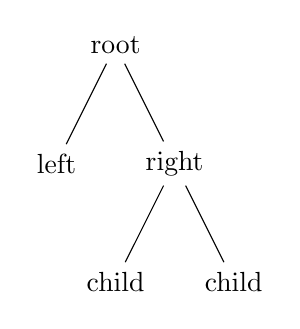
\begin{tikzpicture}
  \node {root}
    child {node {left}}
    child {node {right}
      child {node {child}}
      child {node {child}}
    };
\end{tikzpicture}

A simple image is \tikz \fill (0,0) circle(5pt);.
\end{document}
\end{codeexample}

The method works as follows: if the document is typeset normally, the library searches for replacement images for every picture. Filenames are generated automatically in the default configuration. In our case, the two file names will be |main-figure0| and |main-figure1|. If they exist, those images are simply included and the pictures as such are not processed. If graphics files do not exist, steps are taken to generate the missing ones. Since (currently) only one output file can be set, each missing image needs to be generated by a separate run of \LaTeX\ in which the |\jobname| is set to the desired image file name.
In the default configuration |mode=convert with system call|, these commands are issued automatically by using the |\write18| method to call system commands. It is also possible to output every required file name or to generate a |makefile|; users will need to issue the required commands manually (or with |make|). The probably most comfortable way is to use the default configuration with
\begin{codeexample}[code only]
pdflatex -shell-escape main
\end{codeexample}
\noindent which authorizes |pdflatex| to call itself recursively to generate the images. When it finishes, all images are generated and the document already includes them.


From this point on, successive runs of \LaTeX\ will use the final graphics files, the pictures won't be used anymore. Section~\ref{section-libs-external-nopgf} contains details about how to submit such a file to environments where \pgfname\ is not available.

\begin{command}{\tikzexternalize\oarg{optional arguments}}
	This command activates the externalization. It installs commands to replace every \tikzname-picture. It needs to be called before |\begin{document}| because it may need to install its separate shipout routine.


	The \meta{optional arguments} can be any of the keys described below.

	Note that the generation/modification of auxiliary files like |.aux|, |.toc| etc.\ is usually suppressed while a single image is externalized (details for |\label| support follow).

	It is also possible to write |\tikzexternalize|\marg{main job name} if the argument is delimited by curly braces. This case is mainly for backwards compatibility and is no longer necessary. Since it might be useful in rare circumstances, it is documented in section~\ref{sec:external:detail}.

	A detailed description about the process of externalization is provided in section~\ref{sec:external:detail}.

	\begin{command}{\tikzexternalrealjob}%
		After the library is loaded, this macro will \emph{always} contain the correct main job's name (in the example above, it is |main|). It is to be used instead of |\jobname| when the externalization is in effect.
	\end{command}
	\begin{command}{\pgfactualjobname}
		Once |\tikzexternalize| has been called, |\pgfactualjobname| contains the name of the currently generated output file (which may be |main| or |main-figure0| or |main-figure1| in our example above).
	\end{command}
	\begin{command}{\jobname}
		The value of |\jobname| is one of |\tikzexternalrealjob| or |\pgfactualjobname|, depending on the configuration. In short: if auxiliary file support (|\label| and |\ref|) is activated, |\jobname=\tikzexternalrealjob| (since that's the base file name of auxiliary files).
	\end{command}
\end{command}

\begin{key}{/tikz/external/system call=\marg{template}}
\label{extlib:systemcall:option}
	A template string used to generate system calls. Inside of \marg{template}, the macro |\image| can be used as placeholder for the image which is about to be generated while |\texsource| contains the main file name (in truth, it contains |\input|\marg{main file name}, but that doesn't matter).

	The default is
\begin{codeexample}[code only]
\tikzset{external/system call={pdflatex \tikzexternalcheckshellescape -halt-on-error
    -interaction=batchmode -jobname "\image" "\texsource"}
\end{codeexample}
	\noindent where \declareandlabel{\tikzexternalcheckshellescape} inserts the value of the configuration key |shell escape|
	if and only if the current document has been typeset with |-shell-escape|\footnote{Note that this is always true for the default configuration. This security consideration applies mainly for \texttt{mode=list and make} which will also work \emph{without} shell escapes.}.

	For |eps| output, you can (and need to) use
\begin{codeexample}[code only]
\tikzset{external/system call={latex \tikzexternalcheckshellescape -halt-on-error
    -interaction=batchmode -jobname "\image" "\texsource";
    dvips -o "\image".ps "\image".dvi}}
\end{codeexample}
	
	The argument \marg{template} will be expanded using |\edef|, so any control sequences will be expanded. During this evaluation, `|\\|' will result in a normal backslash, `|\|'. Furthermore, double quotes `|"|', single quotes `|'|', semicolons and dashes `|-|' will be made to normal characters if any package uses them as macros. This ensures compatibility with the |german| package, for example.
\end{key}

\begin{key}{/tikz/external/shell escape=\marg{command-line arg} (initially -shell-escape)}
	Contains the command line option for |latex| which enables the |\write18| feature. For \TeX-Live, this is |-shell-escape|. For Mik\TeX, you should use |\tikzexternalize[shell escape=-enable-write18]|.
\end{key}

\subsubsection{Support for Labels and References In External Files}
The |external| library comes with extra support for |\label| and |\ref| (and other commands which usually store information in the |.aux| file) inside of external files.

There are, however, some points which need your attention when you try to use
\begin{enumerate}
	\item[a)] |\ref| to something in the main document inside of an externalized graphics or
	\item[b)] |\label| in the externalized graphics which is referenced in the main document.
\end{enumerate}

For point a), a |\ref| inside of an externalized graphics works \emph{only} if you issue the required system call \emph{manually} or by |make|. The initial configuration |mode=convert with system call| does \emph{not} support |\ref|. But you can copy--paste the system call generated by |mode=convert with system call| and issue it manually. The reason is that |\ref| information is stored in the main |.aux| file -- but this auxiliary file is not completely written when |mode=convert with system call| is invoked (there is a race condition). Note that |\pageref| is not supported (sorry). Thus: if you have |\ref| inside of external graphics, consider using |mode=list and make| or copy--paste the system call for the image(s) and issue it manually.

Point b) is realized automatically by the external library. In detail, a |\label| inside of an externalized graphics causes the external library to generate separate auxiliary files for every external image. These files are called \meta{imagename}|.dpth|. The extension |.dpth| indicates that the file also contains the image's depth (the |baseline| key of \tikzname). Furthermore, anything which would have been written to an |.aux| file will be redirected to the |.dpth| file -- but only things which occur inside of the externalized |tikzpicture| environment. When the main document loads the image, it will copy the |.dpth| file into the main |.aux| file. Then, successive compilations of the main document contain the external |\label| information. In other words, a |\label| in an external graphics needs the following work flow:
\begin{enumerate}
	\item The external graphics needs to be generated together with its |.dpth| (usually automatically by \tikzname).
	\item The main document includes the external graphics and copies the |.dpth| content into its main |.aux| file.
	\item The main document needs to be translated one further time to re-read its |.aux| file\footnote{Note that it is not possible to activate the content of an auxiliary file after \texttt{\textbackslash begin\{document\}} in \LaTeX.}.
\end{enumerate}
There is just one special case: if a |\label|/|\ref| combination is realized itsself by a |tikzpicture| which should be externalized, you need to proceed as for case a) since |mode=convert with system call| can't handle that stuff on its own. Thus, |\label| works automatically, just translate the main document often enough.



\subsubsection{Customizing the Generated File Names}
The default filename for externalized graphics is `\meta{real file name}|-figure_|\meta{number}' where \meta{number} ranges from $0$ to whatever is required. However, there are a couple of ways to change the generated filenames:
\begin{itemize}
	\item Changing the overall file name using a |prefix|,
	\item Changing the file name for a single figure using |\tikzsetnextfilename|,
	\item Changing the file name for a restricted set of figures using |figure name|.
\end{itemize}

\begin{key}{/tikz/external/prefix=\marg{file name prefix} (initially empty)}
	A shortcut for |\tikzsetexternalprefix|\marg{file name prefix}, see below.
\end{key}

\begin{command}{\tikzsetexternalprefix\marg{file name prefix}}
	Assigns a common prefix used by all file names. For example,
\begin{codeexample}[code only]
\tikzsetexternalprefix{figures/}
\end{codeexample}
	will prepend |figures/| to every external graphics file name.

	Please note that |\tikzsetexternalprefix| is the \emph{only} way to assign a prefix in case you want to prepare your document for environments where \pgfname\ is not installed (see section~\ref{section-libs-external-nopgf}).
\end{command}

\begin{command}{\tikzsetnextfilename\marg{file name}}
	Sets the file name for the \emph{next} \tikzname\ picture or |\tikz| short command. It will \emph{only} be used for the next picture.

	Pictures for which no explicit file name has been set (or the next file name is empty) will get automatically generated file names.

	Please note that |prefix| will still be prepended to \marg{file name}.
\begin{codeexample}[code only]
\documentclass{article}
% main document, called main.tex
\usepackage{tikz}

\usetikzlibrary{external}
\tikzexternalize[prefix=figures/] % activate

\begin{document}

\tikzsetnextfilename{trees}
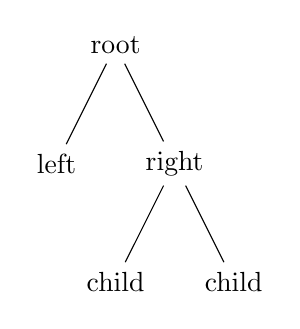
\begin{tikzpicture} % will be written to 'figures/trees.pdf'
  \node {root}
    child {node {left}}
    child {node {right}
      child {node {child}}
      child {node {child}}
    };
\end{tikzpicture}

\tikzsetnextfilename{simple}
A simple image is \tikz \fill (0,0) circle(5pt);. % will be written to 'figures/simple.pdf'


\begin{tikzpicture} % will be written to 'figures/main-figure0.pdf'
   \draw[help lines] (0,0) grid (5,5);
\end{tikzpicture}
\end{document}
\end{codeexample}
\begin{codeexample}[code only]
pdflatex -shell-escape main
\end{codeexample}
\end{command}

\begin{key}{/tikz/external/figure name=\marg{name}}
	Same as |\tikzsetfigurename|\marg{name}.
\end{key}
\begin{command}{\tikzsetfigurename\marg{name}}
	Changes the names of \emph{all} following figures. It is possible to change |figure name| during the document either using |\tikzset{external/figure name|=\marg{name}|}| or with this command. A unique counter will be used for each different \marg{name}, and each counter will start at $0$.

	The value of |prefix| will be applied after |figure name| has been evaluated.
\begin{codeexample}[code only]
\documentclass{article}
% main document, called main.tex
\usepackage{tikz}

\usetikzlibrary{external}
\tikzexternalize % activate

\begin{document}

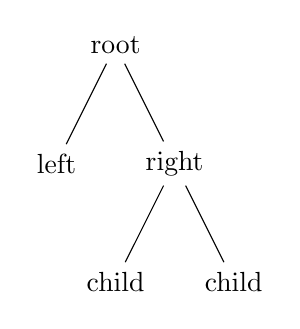
\begin{tikzpicture} % will be written to 'main-figure0.pdf'
  \node {root}
    child {node {left}}
    child {node {right}
      child {node {child}}
      child {node {child}}
    };
\end{tikzpicture}

{
  \tikzsetfigurename{subset_}
  A simple image is \tikz \fill (0,0) circle(5pt);. % will be written to 'subset_0.pdf'

  
\begin{tikzpicture} % will be written to 'subset_1.pdf'
     \draw[help lines] (0,0) grid (5,5);
  \end{tikzpicture}
}% here, the old file name will be restored:

\begin{tikzpicture} % will be written to 'main-figure1.pdf'
   \draw (0,0) -- (5,5);
\end{tikzpicture}
\end{document}
\end{codeexample}
	The scope of |figure name| ends with the next closing brace.

	Remark: Use |\tikzset{external/figure name/.add={prefix_}{_suffix_}}| to add a |prefix_| and a |_suffix_| to the actual value of |figure name|.
\end{command}

\begin{command}{\tikzappendtofigurename\marg{suffix}}
	Appends \meta{suffix} to the actual value of |figure name|.

	It is a shortcut for |\tikzset{external/figure name/.add={}|\marg{suffix}|}| (a shortcut which is also supported if \tikzname\ is not installed, see below).
\end{command}


\subsubsection{Remaking Figures or Skipping Figures}
\begin{command}{\tikzpicturedependsonfile\marg{file name}}
	Adds a dependency for the \emph{next} picture which is about to be externalized. If the command is invoked within a picture environment, it adds a dependency for the surrounding picture. Dependencies are written into \meta{target file}|.dep| in the format
	
	\meta{target file}|.\tikzexternalimgextension: |\meta{file name}.

	The effect is that if \meta{file name} changes, the external graphics associated with the picture shall be remade.

	This command uses the contents of \declareandlabel{\tikzexternalimgextension} to check for graphics. If you encounter difficulties with image extensions, consider redefining this macro (after |\tikzexternalize|).

	\paragraph{Limitations:} this command is currently only supported for |mode=list and make| and the generated |makefile|.
\end{command}
\begin{command}{\tikzexternalfiledependsonfile\marg{external graphics}\marg{file name}}
	A variant of |\tikzpicturedependsonfile| which adds a dependency for an \meta{external graphics}. The argument \meta{external graphics} must be the path as it would have been generated by the external library, i.e.\ without file extension but including any prefixes.
\end{command}

\begin{key}{/tikz/external/force remake=\marg{boolean} (default true)}
	A boolean which is used to customize the up-to-date checks of all following figures. Every up-to-date check will fail, resulting in automatic regeneration of every following figure.

\begin{codeexample}[code only]
\tikzset{external/force remake}

\begin{tikzpicture}
	\draw (0,0) circle(5pt);
\end{tikzpicture}
\end{codeexample}
	You can also use |force remake| inside of a local \TeX\ group to remake only selected pictures. The example
\begin{codeexample}[code only]
\tikz \draw (0,0) -- (1,1);

{
\tikzset{external/force remake}

\begin{tikzpicture}
   \draw (0,0) circle(5pt);
\end{tikzpicture}
}

\tikz \draw (0,0) -- (1,1);
\end{codeexample}
	will only apply |force remake| to the second figure.

	Up-to-date checks are applied for |mode=convert with system call| and the makefile generated by |mode=list and make|.
\end{key}

\begin{key}{/tikz/external/remake next=\marg{boolean} (default true)}
	A variant of |force remake| which applies only to the next image.
\end{key}

\begin{key}{/tikz/external/export next=\marg{boolean} (default true)}
	A boolean which can be used to disable the export mechanism for single pictures.
\end{key}

\begin{key}{/tikz/external/export=\marg{boolean} (initially true)}
	A boolean which can be used to disable the export mechanism for all pictures inside of the current \TeX-scope.

\begin{codeexample}[code only]
\begin{document}
\begin{tikzpicture} % will be exported
	...
\end{tikzpicture}

{
\tikzset{external/export=false}
\begin{tikzpicture} % won't be exported
	...
\end{tikzpicture}
...
}

\begin{tikzpicture} % will be exported
	...
\end{tikzpicture}
\end{document}
\end{codeexample}
	For \LaTeX, the feature lasts until the next |\end|\marg{$\cdot$} (this holds for every call to |\tikzset|).
\end{key}

\begin{command}{\tikzexternaldisable}
	Allows to disable the complete externalization. While |export next| will still collect the contents of picture environments, this command uninstalls the hooks for the external library completely. Thus, nested picture environments or environments where |\end{tikzpicture}| is not directly reachable won't produce compilation failures -- although it is not possible to externalize them automatically.

	The externalization remains disabled until the end of the next \TeX\ group (or environment) or until the next call to |\tikzexternalenable|.
\end{command}

\begin{command}{\tikzexternalenable}
	Re-enables a previously running externalization after |\tikzexternaldisable|.
\end{command}


\subsubsection{Customizing the Externalization}
\begin{key}{/tikz/external/figure list=\marg{boolean} (initially true)}
	A boolean which configures whether a figure list shall be generated. A figure list is an output file named \marg{jobname}|.figlist| which is filled with file names of each figure, one per line.

	This file is not used by \TeX\ anymore, its purpose is to issue the required conversion commands |pdflatex -jobname |\marg{picture file name} \marg{main file} manually (or in a script). See section~\ref{sec:external:detail} for the details about the expected system call (or activate |mode=convert with system call| and inspect you log file).

\begin{codeexample}[code only]
\documentclass{article}
% main document, called main.tex
\usepackage{tikz}

\usetikzlibrary{external}
\tikzexternalize[
   mode=graphics if exists,
   figure list=true,
   prefix=figures/]

\begin{document}

\tikzsetnextfilename{trees}
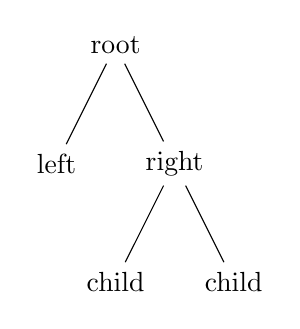
\begin{tikzpicture}
  \node {root}
    child {node {left}}
    child {node {right}
      child {node {child}}
      child {node {child}}
    };
\end{tikzpicture}

\tikzsetnextfilename{simple}
A simple image is \tikz \fill (0,0) circle(5pt);.


\begin{tikzpicture}
   \draw[help lines] (0,0) grid (5,5);
\end{tikzpicture}
\end{document}
\end{codeexample}

\begin{codeexample}[code only]
pdflatex main
\end{codeexample}
generates |main.figlist| containing
\begin{codeexample}[code only]
figures/trees
figures/simple
figures/main-figure0
\end{codeexample}
\end{key}

\begin{key}{/tikz/external/mode=\marg{choice} (initially convert with system call)}
	Configures what to do with \tikzname\ pictures (unless we are currently externalizing one particular image, in that case, these modes are ignored).

	The preconfigured mode |convert with system call| checks whether external graphics files are up-to-date and includes them if that is the case. Any picture which is not up-to-date will be generated automatically using a system call. The system call can be configured using the |system call| template. The up-to-date check is simple: if the file does not exist, it is not up-to-date. Furthermore, if one of the |force remake| or |remake next| keys is true, the figure is not up-to-date. In all other case, the file is considered to be up-to-date. As soon as |convert with system call| is set, the |figure list| will be disabled -- such a file is not required. In case you still need or want it, you can enable it after setting |mode|.

	Please note that system calls may be disabled for security reasons. For pdflatex, they can be enabled using
\begin{codeexample}[code only]
pdflatex -shell-escape
\end{codeexample}
	while other \TeX\ variants may need other switches. The feature is sometimes called |\write18|.
	
	The choice |only graphics| always tries to replace pictures with external graphics. It is an error if the graphics file does not exist.

	The choice |no graphics| (or, equivalently, |only pictures|) typesets \tikzname\ pictures without checking for external graphics.

	A mixture is |graphics if exists|, it checks whether a suitable graphics file exists and includes it if that is the case. If it does not exist, the picture is typeset using \TeX.

	Mode |list only| skips every \tikzname\ picture; it only generates the file \marg{main file}|.figlist| containing file names for every picture, the contents of any picture environment is thrown away and a replacement text is shown. This implies |figure list=true|. See also the |list and make| mode which includes available graphics.

	The mode |list and make| is similar to |list only|: it generates the same file \marg{main file}|.figlist|, but any images which exist already are included as graphics instead of ignoring them. Furthermore, this mode generates an additional file: \marg{main file}.makefile. This allows to use a work flow like
\begin{codeexample}[code only]
% step 1: generate main.makefile:
pdflatex main
% step 2: generate ALL graphics on 2 processors:
make -j 2 main.makefile
% step 3: include the graphics:
pdflatex main
\end{codeexample}
	\noindent This last make method is, however unnecessary: |list and make| just assumes that images are generated somehow (not necessarily with the generated makefile). The generated makefile allows parallel externalization of graphics on multi-core systems and it supports any file dependencies configured with |\tikzpicturedependsonfile|. Furthermore, it respects the |force remake| and |remake next| keys.


\end{key}


\begin{key}{/tikz/external/verbose IO=\marg{boolean} (initially true)}
	A boolean which configures whether I/O operations shall be listed in the logfile.
\end{key}
\begin{key}{/tikz/external/verbose optimize=\marg{boolean} (initially true)}
	A boolean which configures whether optimization operations shall be listed in the logfile.
\end{key}
\begin{key}{/tikz/external/verbose=\marg{boolean} (initially true)}
	Sets all verbosity flags to \meta{boolean}.
\end{key}

\begin{key}{/tikz/external/optimize=\marg{boolean} (initially true)}
	Configures whether the conversion process shall be optimized. This affects only the case when |\jobname| differs from the main file name, i.e. when single pictures are converted.

	In that case, the main file is compiled as usual - but everything except the selected picture is thrown away. If optimization is enabled, all other pictures won't be processed at all. Furthermore, expensive commands which do not contribute to the selected picture will be thrown away as well.

	The default implementation discards |\includegraphics| commands which are \emph{not} inside of the selected picture to reduce conversion time.

	It is possible to add commands which shall be optimized away, see below.
\end{key}

\begin{key}{/tikz/external/optimize command away=\meta{\textbackslash command}\marg{required argument count}}
	Installs commands to optimize \meta{\textbackslash command} away. As is described above, optimization applies to the case when single pictures are converted: one usually doesn't need to process (probably expensive) commands which do not contribute to the selected picture.

	The argument \marg{required argument count} is either empty or a non-negativ integer between $0$ and $9$. It denotes the number of arguments which should be consumed after \meta{\textbackslash command}. In any case, one argument in square brackets after the command will be recognized as well. To be more precise, the following cases for arguments of \meta{\textbackslash command} are supported:
	\begin{enumerate}
		\item If \marg{required argument count} is empty (the default), \meta{\textbackslash command} may take one optional argument in square brackets and one in curly braces (which is also optional).
		\item If \marg{required argument count} is not empty, \marg{\textbackslash command} may take one optional argument in square brackets. Furthermore, it expects exactly \marg{required argument count} following arguments.
	\end{enumerate}

	Example:
\begin{codeexample}[code only]
\tikzset{external/optimize command away=\includegraphics}
\end{codeexample}

\begin{codeexample}[code only]
\newcommand{\myExpensiveMacro}[1]{Very expensive!}

\tikzset{external/optimize command away=\myExpensiveMacro}
\end{codeexample}

\begin{codeexample}[code only]
\newcommand{\myExpensiveMacroWithThreeArgs}[3]{Very expensive!}

\tikzset{external/optimize command away={\myExpensiveMacroWithThreeArgs}{3}}
\end{codeexample}
\begin{codeexample}[code only]
% A command with optional argument:
\newcommand{\aFurtherExample}[3][]{Very expensive!}

% consume only two arguments: the first optional one will be processed
% anyway:
\tikzset{external/optimize command away={\myExpensiveMacroWithThreeArgs}{2}}
\end{codeexample}
	The argument \meta{\textbackslash command} must be the name of a single macro. Any occurrence of this macro, together with its arguments, will be removed.
\begin{codeexample}[code only]
\begin{tikzpicture}
	% this picture is currently converted!
\end{tikzpicture}

This here is outside of the converted picture and contains \myExpensiveMacro. It will be discarded.

This call: \myExpensiveMacro[argument=value]{Argument} as well.
And this here: \myExpensiveMacro{Argument} also.
\end{codeexample}

	The default is to optimize |\includegraphics| away.

	This key is actually a style which sets the |optimize/install| and |optimize/restore| keys.
\end{key}

\begin{key}{/tikz/external/optimize/install}
	A command key which contains code to install optimizations. You can append code here (or clear the macro) if you need to modify the optimization.
\end{key}
\begin{key}{/tikz/external/optimize/restore}
	A command key which contains code to undo optimizations. You can append code here (or clear the macro) if you need to modify the optimization.
\end{key}

\begin{key}{/tikz/external/only named=\marg{boolean} (initially false)}
	If enabled, only pictures for which file names have been set explicitly using |\tikzsetnextfilename| will be considered, no file names will be generated automatically.
\end{key}

\begin{key}{/pgf/images/include external (initially \textbackslash pgfimage\{\#1\})}
\index{External Graphics!Bounding Box Issues}
	This command key constitutes the public interface to exchange the |\includegraphics| command used for the image inclusion. If can be overwritten using |include external/.code=|\marg{\TeX\ code}.

	Its description can be found in the corresponding basic layer documentation on page~\pageref{pgf:includeexternalkey}.

	Just one example here: you can use
\begin{codeexample}[code only]
\pgfkeys{/pgf/images/include external/.code={\includegraphics[viewport=0 0 211.28 175.686]{#1}}}
\end{codeexample}
	to manually change the viewport (bounding box) for included graphics.

	Another example (of probably limited use) is
\begin{codeexample}[code only]
\pgfkeys{/pgf/images/include external/.code={\href{file:#1}{\pgfimage{#1}}}}
\end{codeexample}
	\noindent which will generate a clickable hyperlink around the image. Clicking on it opens the single exported file\footnote{This requires all external graphics files in the same base directory as the main |.pdf| file.}.
	
	If you want to limit the effects of this key to just one externalized figure, use
\begin{codeexample}[code only]
{
  \pgfkeys{/pgf/images/include external/.code={\includegraphics[viewport=0 0 211.28 175.686]{#1}}}
  \begin{tikzpicture}
     ...
  \end{tikzpicture}
}% this brace ends the effect of `include external'
\end{codeexample}
\end{key}

\begin{command}{\tikzifexternalizing\marg{true code}\marg{false code}}
	This command can be used to check whether an image is currently written to its separate graphics file (if the ``grab'' procedure is running). If so, the \marg{true code} will be executed. If not, that means if the main document is being typeset normally, the \marg{false code} will be invoked.

	This command must be used \emph{after} |\tikzexternalize|.
\end{command}

\begin{command}{\tikzifexternalizingnext\marg{true code}\marg{false code}}
	Like |\tikzifexternalizing|, but this variant also checks if the next following figure is the one which is about to be written to its separate graphics file.
\end{command}

\subsubsection{Details About The Process}
\label{sec:external:detail}
The standard run |pdflatex |\meta{main document} causes the |external| library to check every occurrence of |\begin{tikzpicture}| and every |\tikz| shortcommand. If it finds a picture which shall be exported, it queries the respective file name and checks whether the file exists already. If so, it includes the external graphics. If not, it requires an externalization which can be done automatically (the default), semi--automatically (with |mode=list and make|) or manually (by issuing the requires system calls somehow).

The library can detect whether it runs in ``conversion mode'', i.e.\ if it should only process a single image. To do so, it checks whether the internal macro \declareandlabel{\tikzexternalrealjob} exists. If so, its contents is assumed to be \meta{main document} (without the suffix |.tex|). Usually, this macro is set by the conversion system call,
\begin{codeexample}[code only]
pdflatex -jobname "main-figure0" "\def\tikzexternalrealjob{main}\documentclass[a4paper,
               headsepline,footsepline,
               openany,oneside,chapterprefix,
               12pt]
{scrbook}
 
\usepackage{mybooktwo}

\renewcommand\TITLE{My cryptography book}
\renewcommand\AUTHOR{John Doe}
\renewcommand\SHORTAUTHOR{J.~DOE}
\renewcommand\EMAIL{}

\input{thispackages.tex}
\newcommand\qr[2]{\left( \frac{#1}{#2} \right)} % quad rec
\newcommand\Aut{\operatorname{Aut}}
\newcommand\normaleq{\trianglelefteq}
\newcommand\Gal{\operatorname{Gal}}
\newcommand\legendre[2]{\left( \frac{#1}{#2 }\right)}

\newcommand\unit{\varepsilon}
\newcommand\Div{\operatorname{Div}}
\newcommand\ord{\operatorname{ord}}
\newcommand\TT{{\Bbb T}}
\newcommand\LP{\left(}
\newcommand\RP{\right)}
\newcommand\Tr{{\operatorname{Tr}}}

\newtheorem{qn}{Question}  \numberwithin{qn}{section}
\newtheorem{conjecture}{Conjecture}  \numberwithin{conjecture}{section}
\newtheorem{axiom}{Axiom}  \numberwithin{axiom}{section}

%\setlist[itemize]{before=\normalfont} % is this a good idea?

\makeatletter
\newlist{myenum@}{enumerate}{1}
\setlist{nosep,noitemsep,topsep=0pt}
\setlist[itemize]{noitemsep,topsep=0pt}
\setlist[enumerate]{noitemsep,topsep=0pt}
\setlist[myenum@]{label=\normalfont{(\alph*)},ref=\arabic*,nosep,topsep=0pt,partopsep=0pt,parsep=0pt,itemsep=0pt}
\newenvironment{myenum}[1][]
  {\begin{myenum@}[#1]
     }
  {\end{myenum@}}
\makeatother


\textwidth=5.5in
\usepackage{makeidx}

\makeindex

\begin{document}
\topmatter




%\chapter{0}

\chapter{Basic number theory}

\boxpar{
\textsc{Suggestions}.
For this chapter, state the basic axioms and properties/theorems of $\Z$.
Provide proofs. 
But remember that most of the properties/theorems can be generlized
to properties/theorems for rings.
It's still a good idea to prove the facts for $\Z$ since $\Z$ is not
as abstract as general rings and will prepare you for the general results.
}

\section{Axioms of $\Z$}

We will assume that $(\Z, +, \cdot, 0, 1)$ satisfies the following
axioms.
\begin{enumerate}[nosep]
  \li \textsc{Properties of $+$:}
  \begin{enumerate}[nosep]
    \li Closure: If $x, y \in \Z$, then $x + y \in \Z$.
    \li Associativity: If $x, y, z \in \Z$, then $(x + y) + z = x + (y + z)$.
    \li Inverse: If $x \in \Z$, then there is some $y$ such that $x + y = 0 = y + x$.
      The $y$ in the above is an additive inverse of $x$.
    \li Neutrality: If $x \in \Z$, then $0 + x = x = x + 0$.
    \li Commutativity: If $x, y \in \Z$, then $x + y = y + x$.
  \end{enumerate}
  (Memory aid for the first four: CAIN.)
  \li \textsc{Properties of $\cdot$:}
  \begin{enumerate}[nosep]
  \li Closure: If $x, y \in \Z$, then $x \cdot y \in \Z$.
  \li Associativity: If $x, y, z \in \Z$, then $(x \cdot y) \cdot z = x \cdot (y \cdot z)$.
  \li Neutrality: If $x \in \Z$, then $1 \cdot x = x = x + 1$.
  \li Commutativity: If $x, y \in \Z$, then $x \cdot y = y \cdot x$.
  \end{enumerate}
  It is common to write $xy$ instead of $x \cdot y$.

  \li \textsc{Distributivity}:
  If $x, y, z \in \Z$, then
  $x \cdot (y + z) = x \cdot y + x \cdot z$
  and
  $(y + z) \cdot x = y \cdot x + z \cdot x$
    
\end{enumerate}

A set $R$ with operations $+, \cdot$ and elements $0_R, 1_R$ satisfying
the above properties the above is called a commutative ring.
This is an important generalization because there are many
very useful commutative rings and we want to prove results about
commutative rings so that these results can be applied to all
commutative rings, including but not restricted to $\Z$.
And if the commutativity of multiplication is left out, then we have the
concept of a ring; for emphasize these are called non-commutative rings.
This is also an important concept since $n \times n$ matrices with $\R$
entries, $\operatorname{M}_{n \times n}(\R)$, form a non-commutative ring.
In fact, more generally,
the set of $n\times n$ matrices with entries in a commutative ring $R$,
$\operatorname{M}_{n \times n}(R)$,
is itself a non-commutative ring.
We will return to the concept of commutative and non-commutative rings later.

The next property of $\Z$, integrality,
is very special and does not apply to many
communtative rings and is therefore
left out of the definition of commutative ring:
\begin{enumerate}[nosep]
  \li \textsc{Integrality}:
  If $x, y \in \Z$, then
  $xy = 0 \implies x = 0$ or $y = 0$.
\end{enumerate}
Another property of $\Z$ that we will assume is
\begin{enumerate}[nosep]
  \li \textsc{Nontriviality}:
  $0 \neq 1$
\end{enumerate}
This axiom of $\Z$ is extremely simple, but cannot be deduced from
the previous axioms.

The above forms the algebraic properties of $\Z$, i.e., properties involving
addition and multiplication.

It is actually possible to first define axioms for
$\N = \{0, 1, 2, ...\}$ and then define $\Z$ in terms of $\N$.
We will not do that except to mention that the
axioms for $\N$ are called the
\href{https://en.wikipedia.org/wiki/Giuseppe_Peano}{Peano}-\href{https://en.wikipedia.org/wiki/Richard_Dedekind}{Dedekind} axioms
and that one very important Peano-Dedekind axiom of $\N$ is the
\begin{enumerate}[nosep]
  \li \textsc{Well-ordering principle (WOP)} for $\N$:
  If $X$ is a nonempty subset of $\N$, then $X$ contains a minimum element,
  i.e., there is some $m \in X$ such that
  \[
  m \leq x
  \]
  for all $x \in X$.
\end{enumerate}
Without going into details, it can be shown that for $\N$, the WOP
is equivalent to each of the following axioms:
\begin{enumerate}[nosep]
  \li \textsc{Weak Mathematical Induction} for $\N$:
  Let $X$ be a subset of $\N$ satisyfing the following two conditions:
  \begin{enumerate}[nosep]
    \li $0 \in X$ and
    \li Let $n \in \N$. If $n \in X$, then $n + 1 \in X$.
  \end{enumerate}
  Then $X = \N$.
\end{enumerate}
and
\begin{enumerate}[nosep]
  \li \textsc{Strong Mathematical Induction} for $\N$:
  Let $X$ be a subset of $\N$ satisyfing the following two conditions:
  \begin{enumerate}[nosep]
    \li $0 \in X$ and
    \li Let $n \in \N$. If $k \in X$ for all $0 \leq k \leq n$,
    then $n + 1 \in X$.
  \end{enumerate}
  Then $X = \N$.
\end{enumerate}
  
In the above two induction axioms, if we write $X = \{n \mid P(n)\}$ where
$P(n)$ is a propositional formula,
then the induction axioms can be rewritten in the
following way:

\begin{enumerate}[nosep]
  \li \textsc{Weak Mathematical Induction}:
  Let $P(n)$ be a proposition for $n \in \N$ satisyfing the following two
  conditions:
  \begin{enumerate}[nosep]
    \li $P(0)$ is true and
    \li Let $n \in \N$. If $P(n)$ is true, then $P(n+1)$ is true.
  \end{enumerate}
  Then $P(n)$ is true for all $n \in \N$.
\end{enumerate}
and
\begin{enumerate}[nosep]
  \li \textsc{Strong Mathematical Induction}:
  Let $P(n)$ be a proposition for $n \in \N$ satisyfing the following two
  conditions:
  \begin{enumerate}[nosep]
    \li $P(0)$ is true and
    \li Let $n \in \N$. If $k \in X$ for all $0 \leq k \leq n$,
    then $n + 1 \in X$.
    \li Let $n \in \N$. If $P(k)$ is true for $0 \leq k \leq n$,
    then $P(n+1)$ is true.
  \end{enumerate}
  Then $P(n)$ is true for all $n \in \N$.
\end{enumerate}

The above are the algebraic axioms of $\Z$.
There's also the order relation of $\Z$ which is used in WOP
and the two induction principles.
I will formalize the axioms of the order relation later.
For now one can assume that the order relation is defined as follows:
If $x \in \Z$, then
\[
x < y
\]
if there is some $z \in \N$ such that
\[
x + z = y
\]
There is one more axiom of $\Z$ that is related to the
\lq\lq topology" of $\Z$ and uses the order relation:

\begin{enumerate}[nosep]
  \li \textsc{Topology}:
  Given any $x \in \Z$, there is no $y \in \Z$ such that
  \[
  x < y < x + 1
  \]
\end{enumerate}

You can think of topology of a set as study of \lq\lq closeness" of values
in that set.
For $\Q$, given any two distinct
rational values $x < y$, there is also some $z \in \Q$ such that
$x < z < y$.
This is the same for $\R$.
Therefore the topology of $\Z$ is very different from the topology
of $\Q$ and $\R$ because there are \lq\lq holes" in $\Z$ where
there are no $\Z$ values.
$\Z$ has what is called a discrete topology.

The above assume the existence of an order relation on $\Z$, i.e., $<$.
We have to include the following axioms of $<$ on $\Z$.
There is a set $\Z^+$ such that the following holds:
\begin{enumerate}[nosep]
  \li \textsc{Trichotomy}: If $x \in \Z$, then exactly one of the following holds:
  $-x \in \Z^+$, $x = 0$, $x \in \Z^+$.
  \li \textsc{Closure of $+$}: If $x,y \in \Z^+$, then $x + y \in \Z^+$.
  \li \textsc{Closure of $\cdot$}: If $x,y \in \Z^+$, then $x \cdot y \in \Z^+$.
\end{enumerate}
We then define $<$ as follows: If $x, y \in \Z$, then we write $x < y$ if
\[
y - x \in \Z^+
\]
Since $<$ is defined, we can define $x \leq y$ to mean \lq\lq either $x < y$
or $x = y$".
The above order relation is expressed abstractly without refering to the fact that
$\Z^+$ is $\{1, 2, 3, ...\}$, i.e., the set of positive integers.
In fact, you can prove $\Z^+ = \{1, 2, 3, ...\}$ from the above axioms --
see exercises below.

\begin{prop}
  The additive inverse for $x$ is unique.
  In other words, if $y, y'$ satisfies
  \begin{align*}
    x + y &= 0 = y + x \\
    x + y' &= 0 = y' + x \\
  \end{align*}
  Then $y = y'$.
\end{prop}
\proof
TODO

Since the additive inverse of $x$ is unique, we can choose to write
the additive inverse of $x$ in terms of $x$.
This is usually written $-x$.
We define the operator $-$ in terms of the additive inverse:

\begin{defn}
  Let $x,y \in \Z$. We define the subtraction operator as
  \[
  x - y = x + (-y)
  \]
\end{defn}

Note that every $x$ in $\Z$ as an additive inverse, but we did not
require value of $\Z$ to have multiplicative inverse:

\begin{defn}
  Let $x \in \Z$. Then $y$ is a multiplicative inverse of $x$ if
  \[
  x\cdot y = 1 = y\cdot x
  \]
  We say that $x$ is a \defone{unit} if $x$ has a multiplicative inverse.
  We can also say that $x$ is \defone{invertible}.
\end{defn}

Intuitively, you know that the only values of $\Z$ with multiplicative inverses
are $1$ and $-1$.

\begin{prop}
  Let $x \in \Z$.
  If $x$ is a unit, then the multiplicative inverse of $x$ is unique.
  In other words if $y,y'$ satisfies
  \begin{align*}
    x  y &= 1 = y x \\
    x  y' &= 1 = y' x \\
  \end{align*}
  then $y = y'$.
\end{prop}

\begin{defn}
  The multiplicative inverse of $x$, if is exists, is denoted by $x^{-1}$.
\end{defn}

\begin{prop}
  Cancellation law for addition.
  Let $x, y, z \in \Z$.
  \begin{enumerate}[nosep,label=\textnormal{(\alph*)}]
    \item If $x + z = y + z$, then $x = y$.
    \item If $z + x = z + y$, then $x = y$.
  \end{enumerate}
\end{prop}

\begin{prop}
  Let $x \in \Z$.
  \begin{enumerate}[nosep,label=\textnormal{(\alph*)}]
  \item $0x = 0 = x0$
  \item $-0 = 0$
  \item $x - 0 = x$. 
  \end{enumerate}
\end{prop}
\proof
(a) We will first prove $0x = 0$:
\begin{align*}
  0x &= (0 + 0)x & & \text{by Neutrality of $+$} \\
     &= 0x + 0x  & & \text{by Distributivity} \tag{1}
\end{align*}
Since $0x \in \Z$ by Closure of $\cdot$, there is
exists some $y \in \Z$ which is an additive inverse of $0x$, i.e.,
\[
0x + y = 0 = y + 0x \tag{2}
\]
From (1),
\begin{align*}
  y + 0x &= y + (0x + 0x)  \\
  0      &= y + (0x + 0x) & & \text{ by (2)} \\
  0      &= (y + 0x) + 0x & & \text{ by Associativity of $+$} \\
  0      &= 0 + 0x        & & \text{ by (2)} \\
  0      &= 0x            & & \text{ by Neutrality of $+$}
\end{align*}
To prove $0 = x0$, from above
\begin{align*}
  0 &= 0x \\
    &= x0 & & \text{ by Commutativity of $\cdot$}
\end{align*}

(b) TODO

(c) TODO
\qed

\begin{prop}
  Let $x, y \in \Z$.
  \begin{enumerate}[nosep,label=\textnormal{(\alph*)}]
  \item $-(-1) = 1$
  \item $-(-x) = x$
  \item $x(-1) = -x = (-1)x$
  \item $(-1)(-1) = 1$
  \item $(-x)(-y) = xy$
  \end{enumerate}
\end{prop}

\begin{prop}
  Cancellation law for multiplication.
  Let $x, y, z \in \Z$.
  \begin{enumerate}[nosep,label=\textnormal{(\alph*)}]
    \item If $xz = yz$ and $z \neq 0$, then $x = y$.
    \item If $zx = zy$ and $z \neq 0$, then $x = y$.
  \end{enumerate}
\end{prop}

For convenience, I will write $x^2 = xx$ and in general
\[
x^n =
\begin{cases}
  1       &\text{if } n = 0 \\
  x^{n-1}x &\text{if } n > 0 \\
\end{cases}
\]
If $x$ has a multiplicative inverse, i.e., if $x^{-1}$ exists,
then, for $n \geq 0$, I will define
\[
x^{-n} = \left( x^{-1} \right)^n
\]

Note that $nx$ has two meanings: $nx$ can be the multiplication of $n$
and $x$ and it can also be $x + \cdots + x$ with $n$ number of $x$.
Of course you would expect them to be the same.
For now define
\[
  [n]x =
  \begin{cases}
    0       &\text{if } n = 0 \\
    [n-1]x + x &\text{if } n > 0 \\
  \end{cases}
\]
and if $n$ is negative, we define
\[
[n]x = -([-n]x)
\]

\begin{prop}
  Let $x \in \Z$.
  Then $[n]x = n \cdot x$.
\end{prop}


\newpage
\section{Divisibility}
\begin{defn}
  Let $m, n \in \Z$.
  Then we say that $m$ \defterm{divides} $n$, and we write $m \mid n$, if
  there is some $x \in \Z$ such that $mx = n$, i.e.,
  \[
    \exists x \in \Z \cdot [mx = n]
  \]
\end{defn}


\begin{prop}
  Let $a \in \Z$.
  \begin{enumerate}[nosep,label=\textnormal{(\alph*)}]
  \item Then $1 \mid a$.
  \item Then $a \mid 0$.
  \item (Reflexive) $a \mid a$.
  \item If $a \mid b$ and $b \mid a$, then $a = \pm b$.  
  \item (Transitive) If $a \mid b$ and $b \mid c$, then $a \mid c$.
  \item If $a \mid b$, then $a \mid bc$.
  \item If $a \mid b$, $a \mid c$, then $a \mid b + c$.
  \item (Linearity)
    If $a \mid b$, $a \mid c$, then $a \mid bx + cy$ for $x,y \in \Z$.  
  \end{enumerate}
\end{prop}
\proof
TODO

\newpage
\section{Congruences}

\begin{defn}
  Let $a, b \in \Z$ and $N \in \Z$ with $N > 0$.
  Then $a$ is congruent to $b$ mod $N$ and we write
  \[
  a \equiv b \pmod{N}
  \]
  if $N \mid a - b$.
\end{defn}


\begin{prop}
  Let $a,b,c,a',b' \in \Z$.
  \begin{enumerate}[nosep,label=\textnormal{(\alph*)}]
  \item (Reflexivity) $a \equiv a \pmod{N}$
  \item (Symmetry) If $a \equiv b \pmod{N}$, then $b \equiv a \pmod{N}$
  \item (Transitivity)
    If $a \equiv b, b \equiv c \pmod{N}$, then
    $a \equiv c \pmod{N}$
  \item
    If
    $a \equiv b$,
    $a' \equiv b' \pmod{N}$,
    then
    $a + a' \equiv b + b' \pmod{N}$.
  \item
    If
    $a \equiv b$,
    $a' \equiv b' \pmod{N}$,
    then
    $a a' \equiv b b' \pmod{N}$.
  \end{enumerate}
\end{prop}
\proof
TODO

\begin{prop}
  Let $a, N \in \Z$ with $N > 0$.
  Let $q, r \in \Z$ such that
  \[
  a = Nq + r, \,\,\, 0 \leq r < N
  \]
  Then $a \equiv r \pmod{N}$.
\end{prop}
\proof
TODO

\begin{ex}
  Show that the cancellation law for $\Z$ does not translate to $\Z$ mod $N$.
  In other words, find $N, a, b, c$ such that $c \not\equiv 0 \pmod{N}$ and
  \[
  ac \equiv bc \pmod{N}, \,\,\, a \not\equiv b \pmod{N}
  \]
\end{ex}

\newpage\section{Euclidean property}

$\Z$ satisfies this very important property:

\begin{thm}\label{euclideanproperty}
  \textnormal{(\defterm{Euclidean property}\index{Euclidean property}\tinysidebar{Euclidean property})}
  If $a, b \in \Z$ with $b \neq 0$, then there are
  integers $q$ and $r$ 
  satisfying
  \[
  a = bq + r, \,\,\,\,\, 0 \leq |r| < |b|
  \]
\end{thm}

The above theorem is the version that can be generalized to general
rings.
Below is the version for $\Z$.
The only difference is the $|r|$ is replaced by $r$:
\begin{thm}\label{euclideanproperty2}
  \textnormal{(\defterm{Euclidean property 2}\index{Euclidean property 2}\tinysidebar{Euclidean property 2})}
  If $a, b \in \Z$ with $b \neq 0$, then there are
  integers $q$ and $r$ 
  satisfying
  \[
  a = bq + r, \,\,\,\,\, 0 \leq r < |b|
  \]
\end{thm}

In many cases, one is interested in the case when $a \geq 0$.
So this version is the one found in most textbooks:

\begin{thm}\label{euclideanproperty3}
  \textnormal{(\defterm{Euclidean property 3}\index{Euclidean property 3}\tinysidebar{Euclidean property 3})}
  If $a, b \in \Z$ with $a \geq 0, b > 0$, then there are
  integers $q \geq 0$ and $r \geq 0$ 
  satisfying
  \[
  a = bq + r, \,\,\,\,\, 0 \leq r < b
  \]
\end{thm}

$q$ is called the
\defterm{quotient}\index{quotient}\tinysidebar{quotient\\remainder} 
when $a$ is divided by $b$; $r$ is the
\defterm{remainder}\index{remainder}.
$q$ and $r$ are unique (see proposition below).
For instance if $a = 25$ and $b = 3$, then
\[
25 = 3 \cdot 8 + 1, \,\,\,\,\, 0 \leq 1 < 3
\]
The computation
\[
a,b \rightarrow q, r
\]
is called a
\defterm{division algorithm}\index{division algorithm}\tinysidebar{division algorithm}.

In Python, you can do this:
\begin{python}
s = r'''
a = 25
b = 8
q, r = divmod(25, 8)
print("%s = %s * %s + %s" % (a, b, q, r))'''.strip()
f = open('divmod.py', 'w'); f.write(s); f.close()
from latextool_basic import *
print(r'{\footnotesize %s}' % console(s))
print(shell('python divmod.py'))
\end{python}
Algorithmically, when $a$ and $b$ have a huge number of digits
and they are represented using arrays of digits, the division
algorithm to compute $q,r$ is basically long division you learnt in middle
school.
At the hardware level, the same division algorithm occurs but
the computation is in terms of bits and not digits.

If we peek ahead and pretend for the time being that fractions such as 
$\frac{a}{b}$ exists,
then for $a > 0$ and $b > 0$, we have
\[
q = \floor{\frac{a}{b}}, \,\,\,\,\, r = a - bq
\] 
where $\floor{x}$ means the floor of $x$.
If we write $\verb!(a/b)!$ for the
\textit{integer} quotient of $a$ by $b$
(i.e. this is the $/$ in C++ for integers) and $\verb!(a%b)!$
for the corresponding remainder, then of course we have
\[
   \texttt{a = b * (a/b) + (a\%b)}
\]

Although the above Euclidean property is for $\Z$,
We will first prove it for $a \geq 0$ and $b > 0$.
The $q,r$ will satisfy $q \geq 0$, $r \geq 0$.
(Furthermore in this setup $q,r$ are unique.)
Once we have proven the Euclidean property for integer $a \geq 0$,
it will not be difficult to extend the result to the whole of $\Z$.

To prove the Euclidean property of $\Z$, we will use WOP.
(One can also prove the Euclidean property of $\Z$ using induction.)

\textsc{Well-ordering principle for $\N$}\index{Well-ordering principle for $\N$}\tinysidebar{Well-ordering principle for $\N$}:
Let $X$ be a nonempty subset of $\N$. Then $X$ has a minimal element.
In other words there is some $m \in X$ such that
$m \leq x$ for all $x \in X$.

You can prove the following version of
well-ordering principle on $\Z$:

\index{Well-ordering principle for $\Z$}\textsc{Well-ordering principle for $\Z$}\tinysidebar{Well-ordering principle for $\Z$}:
Let $X$ be a nonempty subset of $\Z$ that is \textit{bounded below}.
Then $X$ has a minimal element.
In other words there is some $m \in X$ such that
$m \leq x$ for all $x \in X$.

$\R$ does not satisfy the second version well-ordering principle with $\Z$
replaced by $\R$.
For instance the open interval $X = (0, 1)$ is bounded below (for instance by $-42$).
However there is no $m$ in $X$ such that $m \leq x$ for all $x$ in $X$.
For instance $m = 0.01 \in X$ is not a minimum element of $X$
since $0.0001 \in X$
is smaller than $m$.
Also, $m = 0.0000001 \in X$ is also not a minimum of $X$ since
$0.0000000001 \in X$ is less than $m$.
In fact for any $m \in X$, $(1/2)m$ is in $X$ and is less than $m$.
In other words no value in $X$ can be a minimum value of $X$.

Now we will prove Theorem \ref{euclideanproperty3}.
  
\textit{Proof.}
TODO


\begin{prop}
  Given $a,b$, the $q,r$ in
  Theorem \ref{euclideanproperty3}
  are unique.
  In other words,
  if
  \begin{align*}
    a &= bq+r, \,\,\, 0 \leq r < |b| \\
    a &= bq'+r', \,\,\, 0 \leq r' < |b|
  \end{align*}
  then
  \[
  q=q', \,\,\,\,\, r=r'
  \]
\end{prop}

\proof
From $bq + r = a = bq' + r'$, we have
\begin{align*}
           bq + r = bq' + r'
\end{align*}
If $q = q'$, then $r = r'$.
We now assume $q \neq q'$.
Without loss of generality, we'll assume that $q > q'$.
We have
\[
r' = b(q - q') + r > b + r \geq b
\]
which contradicts $r' < b$.
\qed

Now I'm going to prove Theorem \ref{euclideanproperty}
which allows $a$ to be any integer.

\textit{Proof of Theorem \ref{euclideanproperty}}.
Now I'll use Euclidean Property 3 to prove Euclidean Property 1.
We just need to handle the case when $a < 0$.
Let $u$ be $\pm 1$ so that $ua \geq 0$.
Let $v$ be $\pm 1$ so that $vb > 0$.
Note that $(\pm 1)^2 = 1$, i.e., $u^{-1} = u, v^{-1} = v$.
Using Euclidean Property 3, there exist $q' \geq 0, r'$ such that
\[
a' = b'q' + r', \,\,\, 0 \leq r' < b'
\]
Then
\[
ua = vbq' + r', \,\,\, 0 \leq r' < vb = |b|
\]
Multiplying by $u^{-1}$
\[
a = uvbq' + ur', \,\,\, 0 \leq r' < vb = |b|
\]
and hence
\[
a = b(uvq') + ur', \,\,\, 0 \leq |ur'| < vb = |b|
\]
(Note that $r' \geq 0$ and hence $|ur'| = |u||r'| = r'$.)
Hence if $q = uvq'$ and $r = ur'$, then
\[
a = bq + r, \,\,\, 0 \leq |r| < |b|
\]
and we are done.
\qed


\begin{ex}
  Using the Euclidean property, prove that
  every integer is congruence to $0, 1, 2, \text{ or } 3 \mod{4}$.
\end{ex}

\begin{ex}
  Prove that squares are 0 or 1 mod 4. In other words
  if $a \in \Z$, then $a^2 \equiv 0 \text{ or } 1 \pmod{4}$.
\end{ex}

\begin{ex}
  Solve $4x^3 + y^2 = 5z^2 + 6$ (in $\Z$).
\end{ex}

\begin{ex}
  Prove that $11, 111, 1111, 11111, 111111, ...$ are all
  not perfect squares.
  (An integer is a perfect square is it's of the form
  $a^2$ where $a$ is an integer.)
\end{ex}

\begin{ex}
  How many of $3, 23, 123, 1123, 11123, 111123, 1111123, ...$ are
  perfect squares?
\end{ex}

\newpage\section{Euclidean algorithm -- GCD}

Now let me use the Euclidean property to compute the gcd of two integers.

Let's use the division algorithm on $20$ and $6$.
\[
20 = 6 \cdot 3 + 2, \,\,\,\,\, 0 \leq 2 < 6
\]
Suppose I want to compute $\gcd(20, 6)$.
Of course the example is small enough that we know that it is $2$.
But notice something about this:
\[
20 = 6 \cdot 3 + 2, \,\,\,\,\, 0 \leq 2 < 6
\]
If $d$ is a divisor of $20$ and $6$, then it must also divide
$2$.
Therefore $\gcd(20, 6)$ must divide $2$.
The converse might not be true.
In general, we have this crucial
bridge between Euclidean property and 
common divisors:

\begin{lem}
  \textnormal{(\defone{GCD Lemma})}
  If $a,b,q,r \in \Z$ such that  
  \[
  a = bq + r
  \]
  then
  \[
  \{ d \mid \text{d is a common divisor of $a, b$} \}
  =
  \{ d \mid \text{d is a common divisor of $b, r$} \}
  \]
  Hence
  \[
  \gcd(a,b) = \gcd(b, r)
  \]
\end{lem}
\proof
TODO


In particular, 
given $a, b \in \Z$ where $a > b > 0$.
By the Euclidean property of $\Z$, there exist $q,r \in \Z$ such that
\[
a = bq + r, \,\,\, 0 \leq r < b
\]
Hence
\[
\gcd(a,b) = \gcd(b, r)
\]

Note that in the above, I only require $a = bq + r$.
For instance for to $\gcd(120, 15)$, I can use
$120 = 1\cdot 15 + (120 - 15)$, i.e., $a = 120, b = 15, q = 1, r = 120-15$.
Then $\gcd(120, 15) = \gcd(15, 120-15) = \gcd(15, 105)$.

However if I use the division algorithm, then 
$r$ is \lq\lq small'':
\[
0 \leq r < b
\]
So if you want to compute $\gcd(a,b)$, make sure $a \geq b$ (otherwise
swap them).
Then $\gcd(a, b) = \gcd(b, r)$ and you would have $a \geq b > r$.
So instead of computing $\gcd(a, b)$, you are better off
computing $\gcd(b, r)$.

But like I said, we do not need the $q$ and $r$ to be the quotient
and remainder.
For instance suppose I want to compute the GCD of 514 and 24.
\[
514 = 24 \cdot 1 + (514 - 24)
\]
Then 
\[
\gcd(514, 24) = \gcd(24, 514 - 24)
\]
which gives us
\[
\gcd(514, 24) = \gcd(24, 490)
\]

Note that $\gcd(0, n) = n$ for any positive integer $n$.
I'll let you think about that one.
(Remember what I said before: 0 is in some sense a big number,
like a black hole. Because every positive number divides $0$.)

Of course this gives rise to the following algorithm
\begin{Verbatim}[frame=single,fontsize=\footnotesize]
ALGORITHM: GCD
Inputs: a, b
Output: gcd(a, b)

if b > a:
    swap a, b

if b == 0:
    return a
else:
    return GCD(a - b, b) 
\end{Verbatim}

This only subtracts one copy of $b$ from $a$.
Suppose we can compute
\[
a = bq + r, \,\,\,\,\, 0 \leq r < b
\]
Then
\[
\gcd(a, b) = \gcd(b, r) 
\]
Of course $r$ is the remainder when $a$ is divided by $b$.
Using this we rewrite the above code to get
the
\defterm{Euclidean Algorithm}\index{Euclidean Algorithm}\tinysidebar{Euclidean Algorithm}:
\begin{Verbatim}[frame=single,fontsize=\footnotesize]
ALGORITHM: GCD (Euclidean algorithm)
Inputs: a, b
Output: gcd(a, b)

if b > a:
    # To make sure that for gcd(a,b), a >= b
    swap a, b

if b == 0: 
    return a
else:
    return GCD(b, a % b)
\end{Verbatim}
Note that if \verb!a! $<$ \verb!b!, then
\[
\texttt{GCD(a, b) = GCD(b, a \% b) = GCD(b, a)}
\]
Therefore the swap is not necessary:
\begin{Verbatim}[frame=single,fontsize=\footnotesize]
ALGORITHM: GCD (Euclidean algorithm)
Inputs: a, b
Output: gcd(a, b)

if b == 0: 
    return a
else:
    return GCD(b, a % b)
\end{Verbatim}
In this case, I'm assuming that \verb!a % b! is available.
As an example:
\begin{align*}
  \gcd(514, 24)
  &= \gcd(24, 514 \% 24) = \gcd(24, 10) \\
  &= \gcd(10, 24 \% 10) = \gcd(10, 4) \\
  &= \gcd(10, 10 \% 4) = \gcd(10, 2) \\
  &= \gcd(2, 10 \% 2) = \gcd(2, 0) \\
  &= 2
\end{align*}

The above can also be done in a loop:
\begin{Verbatim}[frame=single,fontsize=\footnotesize]
ALGORITHM: GCD (Euclidean algorithm)
Inputs: a, b
Output: gcd(a, b)

while 1:
    if b == 0: 
        return a
    else:
        a, b = b, a % b
\end{Verbatim}

\begin{ex}
  Compute the following using the Euclidean Algorithm explicitly.
  \begin{enumerate}[nosep,label=\textnormal{(\alph*)}]
  \item $\gcd(10, 1)$
  \item $\gcd(10, 10)$
  \item $\gcd(107, 5)$
  \item $\gcd(107, 26)$
  \item $\gcd(84, 333)$
  \end{enumerate}
\end{ex}

\begin{ex}
  Compute the following.
  You should go as far as you can.
  In other words, either you can a fixed integer (such as $1$) or
  derive the $\gcd(\alpha, \beta)$ where $\alpha, \beta$ are
  as simple as possible.
  For instance, to simplify $\gcd(3 + 2a, a)$, since $3 + 2a = 2 \cdot a + 3$,
  we have
  \[
  \gcd(3 + 2a, a) = \gcd(a, 3)
  \]
  In the following $a, b, x, n \in \Z$ are positive integers.
  \begin{enumerate}[nosep,label=\textnormal{(\alph*)}]
  \item $\gcd(ab, b)$
  \item $\gcd(a, a + 1)$
  \item $\gcd(ab + a, b)$ where $0 < a < b$
  \item $\gcd(a(a+1) + a, (a+1))$ where $0 < a < b$
  \item $\gcd(1 + x + \cdots + x^n, x)$
  \item $\gcd(F_{10}, F_{11})$ where $F_n$ is the $n$--th Fibonacci number.
    (Recall: $F_0 = 1, F_1 = 1, F_{n + 2} = F_{n + 1} + F_n$ for $n \geq 0$.)
  \end{enumerate}
\end{ex}

Despite the fact that the Euclidean algorithm is one of the fastest
algorithm to compute the GCD of two numbers and has been discovered
by
\href{https://en.wikipedia.org/wiki/Euclid}{Euclid} a long time ago (BC 300),
the actual runtime was not known until
\href{https://en.wikipedia.org/wiki/Gabriel_Lam%C3%A9}{Lam\'e}
proved in 1844 that the number of steps to compute
$\gcd(a, b)$ using the Euclidean algorithm
is $\leq 5$ times the number of digits (in base 10 notation)
of $\min(a, b)$.
For instance for the example above
of $\gcd(514, 24)$, the number of digits of $\min(514,24)$ is $2$.
Lam\'e theorem says that the number of steps made by the
Euclidean algorithm in the computation of $\gcd(514, 24)$ is
at most $5 \times 2 = 10$.
The actual number of steps in the earlier computation
\begin{align*}
  \gcd(514, 24)
  &= \gcd(24, 514 \% 24) = \gcd(24, 10) \\
  &= \gcd(10, 24 \% 10) = \gcd(10, 4) \\
  &= \gcd(10, 10 \% 4) = \gcd(10, 2) \\
  &= \gcd(2, 10 \% 2) = \gcd(2, 0) \\
  &= 2
\end{align*}
is 4 (not counting the base case step), i.e.,
\[
  \gcd(514, 24)
 = \gcd(24, 10) \\
 = \gcd(10, 4) \\
 = \gcd(10, 2) \\
 = \gcd(2, 0) \\
\]
Lam\'e's work is generally considered the beginning of
computational complexity theory, which is the study of
resources needed (time or space) to execute an algorithm.
Another fascinating fact about Lam\'e's theorem is that historically
the above proof is the first ever \lq\lq use" of the Fibonacci sequence.

\begin{thm} \textnormal{(Lam\'e 1844)}
  Let $a > b > 0$ be integers.
  If the GCD computation of $a,b$ 
  using Euclidean algorithm results in $n$ steps:
  \[
  \gcd(a_{n+1}, b_{n+1})
  = \gcd(a_{n}, b_{n})
  = \cdots
  = \gcd(a_1, b_1), \,\,\, b_1 = 0
  \]
  where $(a_{n+1}, b_{n+1}) = (a, b)$, and $a_i > b_i$, then
  \begin{enumerate}[nosep,label=\textnormal{(\alph*)}]
  \item  $a \geq F_{n+2}$ and
    $b \geq F_{n+1}$, where $F_n$ are the Fibonacci numbers
    ($F_1 = 1, F_2 = 1, F_3 = 2, F_4 = 3, F_5 = 5$, etc.
    Note that the index starts with $1$.)
  \item $n$ is at most 5 times the number of digits in $b$.
  \end{enumerate}
\end{thm}
\proof
TODO
  
\begin{prop}
  The number of digits of a positive integer $b$ is
  \[
  \floor{\log_{10} b + 1}
  \]
\end{prop}
\proof
TODO

On analyzing the proof, the above is in fact true for any base $> 1$.
In other words the number of base--$B$ symbols to represent $b$ is
\[
\floor{\log_{B} b + 1}
\]
where $B > 1$.
For instance the number of bits needed to represent $b$ is
\[
\floor{\log_{2} b + 1}
\]
For instance, $b = 9_{10} = 1001_2$ which has 4 bits and
\[
\floor{\log_{2} 9 + 1}
= \floor{3.1699... + 1}
= \floor{4.1699...}
= 4
\]

\begin{prop}
  Let positive integer $b$ be written in base $B$ where $B > 1$ is an integer.
  Then the number of base-$B$ symbols used to represent $b$ is
  \[
  \floor{\log_{B} b + 1}
  \]
\end{prop}

\begin{ex}
  Leetcode 650.
  \\
  \url{https://leetcode.com/problems/2-keys-keyboard/}
  \\
  There is only one character \verb!'A'! on the screen of a notepad.
  You can perform one of two operations on this notepad for each step:
  \begin{enumerate}[nosep]
    \li Copy All:
    You can copy all the characters present on the screen (a partial copy is
    not allowed).
    \li Paste: You can paste the characters which are copied last time.
  \end{enumerate}
  Given an integer \verb!n!, return the minimum number of operations to get the character \verb!'A'! exactly \verb!n! times on the screen.
\end{ex}


\begin{ex}
  Leetcode 2447.
  \\
  \url{https://leetcode.com/problems/number-of-subarrays-with-gcd-equal-to-k}
  \\
  Given an integer array \verb!nums! and an integer \verb!k!,
  return the number of subarrays of \verb!nums! where the greatest common
  divisor
  of the subarray's elements is \verb!k!.
  A subarray is a contiguous non-empty sequence of elements within an array.
  The greatest common divisor of an array is the largest integer that evenly
  divides all the array elements.
\end{ex}

\begin{ex}
  Leetcode 1998
  \\
  \url{https://leetcode.com/problems/gcd-sort-of-an-array/}
  \\
  You are given an integer array \verb!nums!,
  and you can perform the following operation any number of times on
  \verb!nums!:
  \begin{enumerate}[nosep]
    \li Swap the positions of two elements \verb!nums[i]! and \verb!nums[j]! if
    \verb!gcd(nums[i], nums[j]) > 1! where \verb!gcd(nums[i], nums[j])! is the
    greatest common divisor of \verb!nums[i]! and \verb!nums[j]!.
  \end{enumerate}
  Return true if it is possible to sort \verb!nums! in non-decreasing order
  using the above swap method, or false otherwise.
\end{ex}

\newpage\section{Extended Euclidean algorithm: GCD as linear combination}

Here's another super important fact:

\begin{thm}
  \textnormal{(\defterm{Extended Euclidean Algorithm}\index{Extended Euclidean Algorithm}\tinysidebar{Extended Euclidean Algorithm})}
If $a$ and $b$ be integers which are not both zero,
then there are integers $x,y$ such that
\[
\gcd(a,b) = ax + by
\]
\end{thm}

The $x,y$ in the above theorem are called
\defterm{B\'ezout's coefficients}\index{B\'ezout's coefficients}\tinysidebar{B\'ezout's coefficients}
of $a,b$.
They are not unique.

\begin{ex}
  Prove that $a \neq 0$, then
  there are many possible $x, y$ such that
  $ax + by = \gcd(a,b)$.
  \qed
\end{ex}
% ax + by = ax + by + ab - ab = a(x + b) + b(y - a).
% ax + by = ax + by + nab - nab = a(x + nb) + b(y - na).


First let me prove that there are $x,y$ such that
\[
ax + by = \gcd(a, b)
\]
The theorem does not give you the algorithm.
Then I'll do a computational example
that compute the gcd of $a,b$ as a linear combination of $a$ and $b$.
The example actually contains the idea behind the algorithm
to compute the B\'ezout's coefficients.
The algorithm is called
the Extended Euclidean Algorithm.

\proof
For convenience, let
me write $(a, b)$ as the set of linear combinations of $a$ and $b$, i.e.,
\[
(a, b) = \{ax + by \mid x,y \in \Z \}
\]
We will also write $(g)$ for the linear combination of $g$, i.e.,
\[
(g) = \{gx \mid x \in \Z \}
\]
(Such linear combinations are called ideals. They are extremely
important in of themselves. Historically, they were created
to study Fermat's last theorem. Since then they are crucial in the
the study of ring theory.)

The proof proceeds in two steps:
\begin{enumerate}[nosep]
\item Given $a,b$ not both zero, there is some $g$ such that
  $(a,b) = (g)$. If $a,b$ are not both zero, $g$ can be chosen to be
  $>0$.
\item The $g$ in the above is in fact $\gcd(a,b)$. 
\end{enumerate}

Now let's prove step 1, i.e., given $a,b$, 
there is some $g$ such that
\[
(a, b) = (g)
\]
First of all if $b = 0$, then by definition
\[
(a, 0) = (a)
\]
and we're done.
Next, we now assume $b \neq 0$.
Then $|b| > 0$.
The set
\[
X = \{ax + by \mid x,y \in \Z \text{ and } ax + by > 0 \} \subseteq \N
\]
is nonempty since it contains
$0\cdot a + 1\cdot |b|$.
By the well-ordering principle of $\N$, $X$ has a minimum element, say $g$.
We will now show that $(a, b) = (g)$.

Since $g$ is a minimum element of $X$, $g$ is in $X$.
Therefore $g = ax + by$.
Hence $gz = a(xz) + b(yz) \in (a, b)$ for all $z \in \Z$.
This implies that $(g) \subseteq (a, b)$.

Now we will prove that $(a, b) \subseteq (g)$.
Let $c \in (a, b)$, i.e., $c = ax + by$ for some $x,y \in \Z$.
Therefore by the Euclidean property of $\Z$, there exists $q,r \in \Z$ such that
\[
c = gq + r, \,\,\, 0 \leq r < g
\]
(Look at the definition of $X$ again. $X$ is a subset of $\N$ so that
$g \geq 1$).
If $r \neq 0$, then
\[
r = c - gq
\]
Note that $c = ax + by$ by our assumption.
We have already shown that $(g) \subseteq (a, b)$, i.e., $g = ax' + by'$.
Therefore, altogether we have
\[
r = c - gq = ax + by - (ax' + b'y)q = a(x-x'q) + b(y-y'q)
\]
Hence $r \in X$.
But $0 \leq r < d$ implies that
\[
r = a(x-x'q) + b(y-b'q)
\]
is an element of $X$ which is less than $g$ which contradicts the
minimality of $g$.
Hence $r = 0$ and we have
\[
c = gq + r = gq \in (g)
\]
We have shown that $(a,b) \subseteq (g)$.

Altogether, we have shown $(a,b) = (g)$.
Step 1 is now completed.

For step 2, we will show that $g$ is the gcd of $a$ and $b$.
Since $(a,b) = (g)$, we have
\[
a \in (a,b) = (g)
\]
i.e., $a = xg$ which means $g$ divides $a$.
Likewise $g$ divides $b$.
Hence $g$ is a common divisor of $a$ and $b$.
Since $(g) \subseteq (a, b)$,
$g = ax_0 + by_0$.
Suppose $d$ is any divisor of $a$ and $b$.
Then $d \mid ax_0 + by_0$ by the linearity of divisibility.
Hence $d \mid g$.
Therefore $g$ is the largest common divisor of $a$ and $b$,
i.e., $g = \gcd(a,b)$.
\qed

The above does not give you an algorithm to compute the
$x$ and $y$.
First let me do an example to show you that
it's possible to compute $\gcd(a,b)$ as a linear combination of $a$ and $b$.
Then I'll give you the algorithm.

Recall that we have computed $\gcd(514, 24) = 2$.
Extended Euclidean Algorithm says that it's possible to find $x$ and $y$
such that
\[
2 = \gcd(514, 24) = 514x + 24y
\]
How do we compute the $x$ and $y$?
Just like the gcd computation (the Euclidean Algorithm),
the $x,y$ are computed using the Euclidean property.
First we have
\begin{align*}
514 = 21 \cdot 24 + 10
\end{align*}
This implies that 
\[
514 \cdot 1 + 24 \cdot (-21) = 10
\]
Now it would be nice if the pesky $10$ goes away and is replaced by
$2$.
How would we do that?
Well look at $24$ and $10$ now.
We have
\[
24 = 2 \cdot 10 + 4
\]
again by Euclidean algorithm.
Multiplying the equation
\[
514 \cdot 1 + 24 \cdot (-21) = 10
\]
throughout by 2 gives us
\[
514 \cdot 2 + 24 \cdot (-42) = 2 \cdot 10
\]
The previous equation
\[
24 = 2 \cdot 10 + 4
\]
say that $2 \cdot 10$ can be replaced by $24 - 4$.
This means that
\[
514 \cdot 2 + 24 \cdot (-42) = 24 - 4
\]
Hmmm ... this says that we have now
\[
514 \cdot 2 + 24 \cdot (-43) = -4
\]
or
\[
514 \cdot (-2) + 24 \cdot 43 = 4
\]
What about 4?
Well, if we look at $10$ and $4$ just like what we did with $24$ and $10$
we would get
\[
10 = 2 \cdot 4 + 2
\]
and the remainder $2$ gives us the GCD!!!
Rearranging it a bit we have
\[
1 \cdot 10 + (-2) \cdot 4 = 2
\]
i.e. 2 is a linear combination of 10 and 4.
But earlier we say that 4 is a linear combination of 514 and 24 ...
\[
514 \cdot (-2) + 24 \cdot 43 = 4
\]
and even earlier we saw that 10 is also a linear combination of 514 and 24 ...
\[
514 \cdot 1 + 24 \cdot (-21) = 10
\]
Surely if we substitute all these values into the equation
\[
1 \cdot 10 + (-2) \cdot 4 = 2
\]
we would get 2 as a linear combination of 514 and 24.
Let's do it ...
\begin{align*}
2 
&= 1 \cdot 10 + (-2) \cdot 4 \\
&= 1 \cdot (514 \cdot 1 + 24 \cdot (-21)) + (-2) (514 \cdot (-2) + 24 \cdot 43) \\
&= 514 \cdot 1 + 24 \cdot (-21) + 514 \cdot 4 + 24 \cdot (-86) \\
&= 514 \cdot 5 + 24 \cdot (-107)
\end{align*}
V\'oila!

\newpage
\begin{ex}
  Using the above idea,
  compute the $\gcd$ and B\'ezout's coefficients of 210 and 78, i.e.,
  compute $x$ and $y$ such that $210x + 78y = \gcd(210, 78)$.
\end{ex}

\newpage
\begin{ex}
Analyze the above and design an algorithm 
so that when given $a$ and $b$, the algorithm computes
$x$ and $y$ such that $ax + by = \gcd(a,b)$.
\end{ex}

\newpage
To help you analyze the above computation,
let me organize our computations a little.
If we can make the process systematic, then there is hope that we can 
make the idea work for all $a$ and $b$, i.e., then we would have an
algorithm and hence can program it and compute it's runtime performance.

We know for sure that we have to continually use
Euclidean property on pairs of numbers.
So here we go:
\begin{align*}
514 &= 21 \cdot 24 + 10 \\
24  &= 2 \cdot 10 + 4 \\
10  &= 2 \cdot 4 + 2 \\
4   &= 2 \cdot 2 + 0
\end{align*}
Note that this corresponds to the $\gcd$ computation
\begin{align*}
\gcd(514, 24) 
&= \gcd(24, 514 - 21 \cdot 24) = \gcd(24, 10) \\
&= \gcd(10, 24 - 2 \cdot 10) = \gcd(10, 4) \\
&= \gcd(4, 10 - 2 \cdot 4) = \gcd(4, 2)  \\
&= \gcd(2, 4 - 2\cdot 2) = \gcd(2, 0) \\
&= 2
\end{align*}
So in the computation
\begin{align*}
514 &= 21 \cdot 24 + 10 \\
24  &= 2 \cdot 10 + 4 \\
10  &= 2 \cdot 4 + 2 \\
4   &= 2 \cdot 2 + 0
\end{align*}
if the remainder is $0$ (see the last line), 
then the previous line's remainder must be the gcd.

Let's look at our computation of the gcd of $514$ and $24$:
\begin{align*}
514 &= 21 \cdot 24 + 10 \\
24  &= 2 \cdot 10 + 4 \\
10  &= 2 \cdot 4 + 2 \\
4   &= 2 \cdot 2 + 0
\end{align*}
Recall that the above computation means that the gcd is 2.
Note only that through backward substitution, we can rewrite
$2$ as a linear combination of $514$ and $24$.

Let's try to do this in a more organized way.
So here's our facts again:
\begin{align*}
514 &= 21 \cdot 24 + 10 \\
24  &= 2 \cdot 10 + 4 \\
10  &= 2 \cdot 4 + 2 
\end{align*}
Let me put the remainders on one side:
\begin{align*}
10 &= 514 - 21 \cdot 24 \tag{1} \\
4  &= 24  - 2 \cdot 10  \tag{2} \\
2  &= 10  - 2 \cdot 4   \tag{3} \\
\end{align*}
Note that (1) tells you that
$10$ is a linear combination of $514,24$.
(2) tells you that $4$ is a linear combination of $24,10$.
If we substitute (1) into (2), $4$ will become a linear
combination of $514,24$.
(3) says that $2$ is a linear combination of $10,4$.
But $10$ is a linear combination of $514,24$
and $4$ is a linear combination of $514,24$.
Hence $2$ is also a linear combination of $514,24$.
See it?

OK. Let's do it.
From
\begin{align*}
10 &= 514 - 21 \cdot 24 \tag{1} \\
4  &= 24  - 2 \cdot 10  \tag{2} \\
2  &= 10  - 2 \cdot 4   \tag{3} \\
\end{align*}
if we substitute (1) into (2) and (3) (i.e., rewrite $10$ as a linear
combination of $514,24$):
\begin{align*}
10 &= 514 - 21 \cdot 24 \tag{1} \\
4  &= 24  - 2 \cdot (514 - 21 \cdot 24)  \tag{2} \\
2  &= (514 - 21 \cdot 24)  - 2 \cdot 4   \tag{3} 
\end{align*}
Collecting the multiples of 514 and 24:
\begin{align*}
10 &= 514 - 21 \cdot 24 \tag{1} \\
4  &= (-2) \cdot 514 + (1 + (-2)(-21)) \cdot 24  \tag{2'} \\
2  &= (1) \cdot 514 + (-21) \cdot 24  - 2 \cdot 4   \tag{3'} 
\end{align*}
and simplifying:
\begin{align*}
10 &= 514 - 21 \cdot 24 \tag{1} \\
4  &= (-2) \cdot 514 + (43) \cdot 24  \tag{2'} \\
2  &= (1) \cdot 514 + (-21) \cdot 24  - 2 \cdot 4   \tag{3'} 
\end{align*}
Substituting (2$'$) into (3$'$):
\begin{align*}
10 &= 514 - 21 \cdot 24 \tag{1} \\
4  &= (-2) \cdot 514 + (43) \cdot 24  \tag{2'} \\
2  &= (1) \cdot 514 + (-21) \cdot 24  - 2 \cdot ((-2) \cdot 514 + (43) \cdot 24)  \tag{3'} 
\end{align*}
Tidying up:
\begin{align*}
10 &= 514 - 21 \cdot 24 \tag{1} \\
4  &= (-2) \cdot 514 + (43) \cdot 24  \tag{2'} \\
2  &= (1 - 2(-2)) \cdot 514 + (-21 - 2(43)) \cdot 24 \tag{3''} 
\end{align*}
Simplifying:
\begin{align*}
10 &= 514 - 21 \cdot 24 \tag{1} \\
4  &= (-2) \cdot 514 + (43) \cdot 24  \tag{2'} \\
2  &= (5) \cdot 514 + (-107) \cdot 24 \tag{3''}
\end{align*}

(It's a good idea to check after each substitution that
the equalities still hold. We all make mistakes, right?)

OK.
That's great.
It looks more organized now.
So much so that you can now easily write a program to compute
the above.


Now let's look at the general case.
Suppose instead of $514$ and $24$, we write $a$ and $b$.
The computation will look like this:
\begin{align*}
a   &= q_1 \cdot b   + r_1 \\
b   &= q_2 \cdot r_1 + r_2 \\
r_1 &= q_3 \cdot r_2 + r_3 \\
r_2 &= q_4 \cdot r_3 + 0
\end{align*}
To make things even more regular and uniform, let me rewrite it this way:
\begin{align*}
r_0 &= q_1 \cdot r_1 + r_2 \\
r_1 &= q_2 \cdot r_2 + r_3 \\
r_2 &= q_3 \cdot r_3 + r_4 \\
r_3 &= q_4 \cdot r_4 + 0
\end{align*}
A lot nicer, right?
Let me write it this way with the remainder term on the lefts:
\begin{align*}
r_2 &= (1) \cdot r_0 + (-q_1) \cdot r_1 \\
r_3 &= (1) \cdot r_1 + (-q_2) \cdot r_2 \\
r_4 &= (1) \cdot r_2 + (-q_3) \cdot r_3 
\end{align*}
(Remember that $r_4$ is the gcd ... $r_0 = 514, r_1 = 24$ ... right?)
Organized this way, we have the gcd on one side of the equation.
Now if we substitute the first equation into the second we get
\begin{align*}
r_2 &= (1) \cdot r_0 + (-q_1) \cdot r_1 \text{ ... USED }\\
r_3 &= (1) \cdot r_1 + (-q_2) \cdot ((1) \cdot r_0 + (-q_1) \cdot r_1) \\
r_4 &= (1) \cdot r_2 + (-q_3) \cdot r_3 
\end{align*}
i.e.,
\begin{align*}
r_2 &= (1) \cdot r_0 + (-q_1) \cdot r_1 \text{ ... USED }\\
r_3 &= (-q_2) \cdot r_0 + (1 + q_1q_2) \cdot r_1 \\
r_4 &= (1) \cdot r_2 + (-q_3) \cdot r_3  
\end{align*}
Note that we cannot throw away the first equation yet.
We need to keep $r_2$ around since it appears in the third equation!
So when can we throw the first equation away?
Look at the general case.
Suppose we have
\begin{align*}
r_2 &= (1) \cdot r_0 + (-q_1) \cdot r_1  \\
r_3 &= (1) \cdot r_1 + (-q_2) \cdot r_2  \\
r_4 &= (1) \cdot r_2 + (-q_3) \cdot r_3  \\
r_5 &= (1) \cdot r_3 + (-q_4) \cdot r_4  \\
r_6 &= (1) \cdot r_4 + (-q_5) \cdot r_5  \\
...
\end{align*}
Aha! $r_2$ is used only in the next \textit{two} equations.

Suppose we are at equation 3:
\begin{align*}
r_3 &= c_1 \cdot r_0 + d_1 \cdot r_1  \\
r_4 &= c_2 \cdot r_0 + d_2 \cdot r_1 
\end{align*}
We have to compute the next equation:
This requires $r_3, r_4$.
Then we have
\[
r_5 = (1) \cdot r_3 + (-q_4) \cdot r_4
\]
where
\[
q_4 = \floor{r_3/r_4}, \,\,\,\,\, r_5 = r_3 - q_4r_4
\]
Altogether we have
\begin{align*}
r_3 &= c_1 \cdot r_0 + d_1 \cdot r_1     \\
r_4 &= c_2 \cdot r_0 + d_2 \cdot r_1     \\
r_5 &= (1) \cdot r_3 + (-q_4) \cdot r_4 
\end{align*}
The last equation becomes
\begin{align*}
r_5 &= c_1 \cdot r_0 + d_1 \cdot r_1  
+ 
(-q_4) \cdot (c_2 \cdot r_0 + d_2 \cdot r_1)
\end{align*}
i.e.
\begin{align*}
r_5 &= (c_1 - q_4 c_2) \cdot r_0 + (d_1 - q_4 d_2) \cdot r_1 
\end{align*}

Let me repeat that in a slightly more general context.
If we have
\begin{align*}
r_3 &= c_1 \cdot r_0 + d_1 \cdot r_1  \\
r_4 &= c_2 \cdot r_0 + d_2 \cdot r_1 
\end{align*}
then we get (throwing away the first equation):
\begin{align*}
r_4 &=c_2 \cdot r_0 + d_2 \cdot r_1 \\
r_5 &= (c_1 - q_4 c_2) \cdot r_0 + (d_1 - q_4 d_2) \cdot r_1 
\end{align*}
To put it in terms of numbers instead of equations this is what we get:
If we have
\[
c_1, d_1, c_2, d_2, r_3, r_4
\]
then we get
\[
c_2, d_2, 
c_1 - \floor{r_3/r_4} c_2, 
d_1 - \floor{r_3/r_4}d_2, 
r_4, r_3 - \floor{r_3/r_4}r_4
\]
In general, if we have
\[
c, d, c', d', r, r'
\]
then we get
\[
c', d', 
c - \floor{r/r'} c', d - \floor{r/r'}d', 
r', r - \floor{r/r'}r'
\]

Of course since we start off with $r_0, r_1$ (i.e. what we call $a$ and $b$
above), we have
\begin{align*}
r_0 &= 1 \cdot r_0 + 0 \cdot r_1 \\
r_1 &= 0 \cdot r_0 + 1 \cdot r_1 \\
\end{align*}
i.e., you would start off with
\[
c=1, d=0, c'=0, d'=1, r=r_0, r'=r_1
\]
Let's check this algorithm with our $r_0 = 514, r_1 = 24$.

STEP 1: The initial numbers are
\[
c=1, d=0, c'=0, d'=1, r=514, r'=24
\]
Again this corresponds to
\begin{align*}
r_3 &= 1 \cdot 514 + 0 \cdot 24  \\
r_4 &= 0 \cdot 514 + 1 \cdot 24 \\
\end{align*}

STEP 2: 
The new numbers (6 of them) are
\begin{align*}
 c' &=0 \\
 d' &=1 \\
 c - \floor{r/r'} c' &= 1 - \floor{514/24} 0 = 1\\
 d - \floor{r/r'}d' &= 0 - \floor{514/24}1 = 0 - 21 = -21 \\
 r' &= 24 \\ 
 r - \floor{r/r'}r' &= 514 - \floor{514/24}24 = 514 - 504 = 10
\end{align*}
So the new numbers (we reset the variables in the algorithm):
\[
c=0, d=1, c'=1, d'=-21, r=24, r'= 10
\]
These corresponds to the data on the second and third line of the following:
\begin{align*}
514 &= 1 \cdot 514 + 0 \cdot 24      \\
24  &= 0 \cdot 514 + 1 \cdot 24      \\
10  &= 1 \cdot 514 + (-21) \cdot 24 
\end{align*}

STEP 3: From the 6 numbers from STEP 2 we get
\begin{align*}
 c' &= 1 \\
 d' &= -21 \\
 c - \floor{r/r'} c' &= 0 - \floor{24/10} 1 = -2 \\
 d - \floor{r/r'}d'  &= 1 - \floor{24/10} (-21) = 1 + 42 = 43 \\
 r' &= 10 \\ 
 r - \floor{r/r'}r' &= 24 - \floor{24/10}10 = 24 - 20 = 4
\end{align*}
So the new numbers (we reset the variables in the algorithm):
\[
c=1, d=-21, c'=-2, d'= 43, r=10, r'= 4
\]
These corresponds to the data on the third and fourth line of the following:
\begin{align*}
514 &= 1 \cdot 514 + 0 \cdot 24     \\
24  &= 0 \cdot 514 + 1 \cdot 24     \\
10  &= 1 \cdot 514 + (-21) \cdot 24 \\
4   &= (-2) \cdot 514 + 43 \cdot 24 
\end{align*}

STEP 4: From the 6 numbers from STEP 3 we get
\begin{align*}
 c' &= -2 \\
 d' &= 43 \\
 c - \floor{r/r'} c' &= 1 - \floor{10/4} (-2) = 1 + 4 = 5 \\
 d - \floor{r/r'}d'  &= -21 - \floor{10/4} (43) = -21 - 86 = -107 \\
 r' &= 4 \\ 
 r - \floor{r/r'}r' &= 10 - \floor{10/4} 4 = 10 - 8 = 2
\end{align*}
So the new numbers (we reset the variables in the algorithm):
\[
c = -2, d = 43, c' = 5, d'= -107, r=4, r'= 2
\]
These corresponds to the data on the fourth and fifth line of the following:
\begin{align*}
514 &= 1 \cdot 514 + 0 \cdot 24      \\
24  &= 0 \cdot 514 + 1 \cdot 24      \\
10  &= 1 \cdot 514 + (-21) \cdot 24  \\
4   &= (-2) \cdot 514 + 43 \cdot 24  \\
2   &= 5 \cdot 514 + (-107) \cdot 24 
\end{align*}

STEP 5: From the 6 numbers from STEP 4 we get
\begin{align*}
 c' &= 5 \\
 d' &= -107 \\
 c - \floor{r/r'} c' &= -2 - \floor{4/2} 5 = -2 - 10 = -12 \\
 d - \floor{r/r'} d'  &= 43 - \floor{4/2} (-107) = 43 + 214 = 257 \\
 r' &= 2 \\ 
 r - \floor{r/r'}r' &= 4 - \floor{4/2} 2 = 4 - 4 = 0
\end{align*}
So the new numbers (we reset the variables in the algorithm):
\[
c = 5, d = -107, c' = -12, d'= 257, r=2, r'= 0
\]
These corresponds to the data on the fifth and sixth line of the following:
\begin{align*}
514 &= 1 \cdot 514 + 0 \cdot 24       \\
24  &= 0 \cdot 514 + 1 \cdot 24       \\
10  &= 1 \cdot 514 + (-21) \cdot 24   \\
4   &= (-2) \cdot 514 + 43 \cdot 24   \\
2   &= 5 \cdot 514 + (-107) \cdot 24  \\
0   &= (-12) \cdot 514 + 257 \cdot 24 
\end{align*}

Of course (as before) at this point, you see that the $r'=0$.
Therefore 
\[
\gcd(514, 24) = 2
\]
and furthermore from $c=5, d=-107$, we get
\[
5 \cdot 514 + (-107) \cdot 24 = \gcd(514, 24) 
\]

Here's a Python implementation with some test code:
\begin{Verbatim}[frame=single, fontsize=\small]
ALGORITHM: EEA
INPUTS: a, b
OUTPUTS: r, c, d where r = gcd(a, b) = c*a + d*b

a0, b0 = a, b
d0, d = 0, 1
c0, c = 1, 0
q = a0 // b0
r = a0 - q * b0

while r > 0:
    d, d0 = d0 - q * d, d    
    c, c0 = c0 - q * c, c

    a0, b0 = b0, r
    q = a0 // b0
    r = a0 - q * b0

r = b0
return r, c, d
\end{Verbatim}
You can pound real hard at the Extended Euclidean Algorithm with this:

By the way, this is somewhat similar to what we call
\textit{tail recursion} (CISS445)
an extremely important technique in functional programming.
All LISP hackers and people working in high performance computing
and compilers swear by it.
You don't see recursion in the above code, but you can 
replace the while-loop with recursion and if
you have a compiler/interpreter that can perform 
true tail recursion, then it would run exactly like the above algorithm.

\begin{ex}
  Leetcode 365 \\
  \url{https://leetcode.com/problems/water-and-jug-problem/description/} \\
  (Also, Die Hard 3 problem
  \url{https://www.math.tamu.edu/~dallen/hollywood/diehard/diehard.htm}.)
  You are given two jugs with capacities \verb!jug1Capacity! and
  \verb!jug2Capacity! liters.
  There is an infinite amount of water supply available.
  Determine whether it is possible to measure exactly \verb!targetCapacity!
  liter using these two jugs.

  If \verb!targetCapacity! liters of water are measurable,
  you must have \verb!targetCapacity! liters of water contained within one or
  both buckets by the end.

  Operations allowed:
  \begin{enumerate}[nosep]
    \item Fill any of the jugs with water.
    \item Empty any of the jugs.
    \item Pour water from one jug into another till the other jug is completely
      full, or the first jug itself is empty.
  \end{enumerate}
  
\end{ex}

You'll see that there are times when you're only interested in 
the value of $x$ and not $y$ (or $y$ and not $x$ -- the above is symmetric
about $x$ and $y$).
Do you notice $x$ comes from $c$?
If you analyze the above algorithm, you see immediately that $c$
is computed from $c'$ and $c'$ is computed from $c,c',q$, 
$q$ is computed from $r, r'$, $r$ is computed from $r'$,
and finally (phew!) $r'$ is computed from $r, q, r'$.
Therefore if you're interested in $c$, you don't need to compute $d$ 
or $d'$.
So you can change the EEA to this:

\begin{Verbatim}[frame=single, fontsize=\small]
ALGORTHM: EEA2 (sort of EEA ... without the d, d0)
INPUTS: a, b
OUTPUTS: r, c where r = gcd(a, b) = c*a + d*b for some d

a0, b0 = a, b
c0, c = 1, 0
q = a0 // b0
r = a0 - q * b0

while r > 0:   
    c, c0 = c0 - q * c, c

    a0, b0 = b0, r
    q = a0 // b0
    r = a0 - q * b0

r = b0
return r, c
\end{Verbatim}

Later you'll see why we compute only $c$.
It's not that we have something against $d$.

\newpage
\begin{ex}
  Compute the following gcd and the B\'ezout's coefficients of the
  given numbers by following the Extended Euclidean Algorithm.
  \begin{enumerate}[nosep]
  \item $\gcd(0, 10)$
  \item $\gcd(10, 0)$
  \item $\gcd(10, 1)$
  \item $\gcd(10, 10)$
  \item $\gcd(107, 5)$
  \item $\gcd(107, 26)$
  \item $\gcd(84, 333)$
  \item $\gcd(F_{10}, F_{11})$ where $F_n$ is the $n$--th Fibonacci number.
    (Recall: $F_0 = 0, F_1 = 1, F_{n + 2} = F_{n + 1} + F_n$.)
  \item $\gcd(ab, b)$
  \item $\gcd(a, a + 1)$
  \item $\gcd(ab + a, b)$ where $0 < a < b$. Go as far as you can.
  \item $\gcd(a(a+1) + a, (a+1))$ where $0 < a < b$. Go as far as you can.
  \end{enumerate}
\end{ex}

\begin{ex}
  Prove that if $a \mid c$, $b \mid c$, and $\gcd(a,b) = 1$, then
  $ab \mid c$.
\end{ex}

\begin{ex}
  Prove that if $a \mid c$, $b \mid c$, then
  \[
  \frac{ab}{\gcd(a,b)} \mid c
  \]
\end{ex}


\begin{ex}
  Leetcode 920.\\
  \url{https://leetcode.com/problems/number-of-music-playlists}\\
  Your music player contains n different songs.
  You want to listen to goal songs (not necessarily different) during your trip.
  To avoid boredom, you will create a playlist so that:
  \begin{enumerate}[nosep]
    \li Every song is played at least once.
    \li A song can only be played again only if k other songs have been played.
  \end{enumerate}
  Given \verb!n!, \verb!goal!, and \verb!k!,
  return the number of possible playlists that you can create.
  Since the answer can be very large, return it modulo $109 + 7$.
\end{ex}

\newpage\section{Primes}

\begin{defn}
A prime $p$ is a positive integer greater than 1 that is
divisible by only 1 and itself.
In other words $p \in \N$ is a
\defterm{prime}\index{prime}\tinysidebar{prime}
if $p > 1$ and 
if $d \mid p$, then $d = 1$ or $d = p$.
\end{defn}

Examples of primes are $2, 3, 5, 7, 11, 13, 17, 19, ...$.

Integers least zero can be divided into the following types:
\begin{enumerate}[nosep]
  \li $0$ -- the zero element
  \li $1$ -- the unit element (i.e. the only invertible element $\geq 0$)
  \li primes -- $2, 3, 5, 7, 11, ...$
  \li \defone{composites} -- integers $> 1$ which are not primes 
\end{enumerate}

(
Instead of primes of $\N \cup \{0\}$,
it's also possible to define primes of $\Z$.
A prime of $\Z$ is an integer not $-1, 0, 1$
such that if $d \mid p$, then $d = \pm 1$ or $d = \pm p$.
In that case primes of $\Z$ are
$\pm 2, \pm 3, \pm 5, \pm 7, \pm 11, ...$.)


\begin{prop} \textnormal{(Euclid)}
  There are infinitely many primes.
\end{prop}

\proof
TODO


\begin{prop} \textnormal{(Euclid)}
  There are arbitrarily long consecutives integers of composites.
\end{prop}

\proof
$n!+2$,
$n!+3$,
$n!+4$,
$\ldots$,
$n!+n$
are all composities for $n \geq 2$.
This list is therefore a list of consecutive composites of length
$n - 1$.
\qed


The follow lemma is extremely important and is used
for instance in the fundamental theorem of arithmetic to prove
the uniqueness of prime factorization in $\N$ (or $\Z$).
To break tradition, we will call this a theorem (instead of a lemma):

\begin{thm}
  \textnormal{(\defone{Euclid's lemma})}
  If $p$ is a prime and $p \mid ab$, then either $p \mid a$ or $p \mid b$.
\end{thm}

\proof
TODO


The above generalizes easily (by induction) to the following:


\begin{cor}
If $p$ is a prime and $p \mid a_1 a_2 \cdots a_n$, then 
$p$ divides at least one of the $a_1, \ldots, a_n$.
\end{cor}
\proof
We will prove this by strong induction on the number of terms
in $a_1, ..., a_n$.
Hence let $P(n)$ be the above statement, i.e., $P(n)$ is the
statement that if a prime divides the product of $n$ terms,
then $p$ divides at least one of the terms.

The case of $n = 2$ is Euclid's lemma.
Hence $P(2)$ holds.
This is the base case of our induction.

Now assume $P(k)$  is true for $2 \leq k \leq n$.
Let $p$ be a prime divide $a_1 a_2 \cdots a_n a_{n + 1}$.
Therefore $p$ divides $a_1 a_2 \cdots a_{n-1} b$ (there are $n - 1$ terms)
where $b = a_n a_{n + 1}$.
Since $P(n)$ is true, $p$ divides at least one of $a_1, ..., a_{n - 1}, b$.
Since $P(2)$ is true,
$p$ divides $b = a_n a_{n + 1}$ if $p$ divides $a_n$ or $a_{n + 1}$.
Hence $p$ divides at least one of $a_1, ..., a_{n + 1}$.
Therefore $P(n + 1)$ holds.
\qed

\begin{thm} \textnormal{(Euclid's \defone{Fundamental Theorem of Arithmetic})}
Every positive integer $> 1$ can be written as a unique product of primes
up to permutation of the prime factors.
This means
\begin{enumerate}[nosep,label=\textnormal{(\alph*)}]
\item[(a)] If $n > 1$ is an integer, then $n$ can be written as a product
of primes.
\item[(b)] If $n$ is written as two products of primes:
\[
n = p_1 p_2 \cdots p_k = q_1 q_2 \cdots q_\ell
\]
where $p_i$ and $q_j$ are primes arranged in ascending order, i.e.,
\begin{align*}
p_1 \leq p_2 \leq \cdots \leq p_k \\
q_1 \leq q_2 \leq \cdots \leq q_\ell
\end{align*}
then $k = \ell$ and 
\[
p_1 = q_1, \,\,\,\,\,
p_2 = q_2, \,\,\,\,\,
\cdots, \,\,\,\,\,
p_k = q_k, \,\,\,\,\,
\]
\end{enumerate}
\end{thm}

\proof
TODO

The statement of the Fundamental Theorem of Arithmetic can include
the case of $n = 1$ if we accept that the product of an empty
set of integers is $1$:
\[
\prod_{p \in \{\}} p = 1
\]

\begin{prop} Let $a = \prod_{p \in P} p^{a_p}$, $b = \prod_{p
    \in P} p^{b_p}$ and $c = \prod_{p \in P} p^{c_p}$
  where $P$ is a finite set of primes. Then
\begin{enumerate}[nosep,label=\textnormal{(\alph*)}]
 \item $c = ab$ $\implies$ $c_p = a_p + b_p$.
 \item $a \mid b$ $\implies$ $a_p \leq b_p$ for all $p \in P$.
 \item $c = \gcd(a,b)$ $\implies$ $c_p = \min(a_p, b_p)$.
\end{enumerate}
\end{prop}

The above assumes the easily proven facts that
\[
\prod_{p \in P} p^{a_p}
\prod_{p \in P} p^{b_p}
=
\prod_{p \in P} p^{a_p + b_p}
\]
(by commutativity of $\cdot$) and
\[
\prod_{p \in P} p^{a_p}
=
\prod_{p \in P} p^{b_p}
\implies
a_p = b_p \text{ for all $p \in P$}
\]
by uniqueness of prime factorization from the Fundamental Theorem of Arithmetic.
Here, $P$ is a set of distinct primes.


\begin{prop}
  If $n > 1$ is not a prime, then there is a prime factor $p$ such that
  $p \leq \sqrt{n}$.
\end{prop}
\proof
TODO
\qed

Therefore a very simple primality test algorithm for $n$ is the following:
  
\begin{Verbatim}[fontsize=\footnotesize,frame=single]
ALGORITHM: BRUTE-FORCE-PRIMALITY-TEST
INPUT: n
OUTPUT: true if n is prime. If n < 2, false is returned.

if n < 2: return false

d = 2
while d <= sqrt(n):
    if n % d == 0:
        return false
    d = d + 1
return true
\end{Verbatim}

In terms of $n$, the runtime is $O(\sqrt{n})$.
However in terms of the bits of $n$, by Proposition 1.5.2,
the number of $n$ is
\[
b = \floor{\log_2 ( n + 1 )} = \log_2(n + 1) - \alpha
\]
where $0 \leq \alpha < 1$.
Hence
\[
n = 2^b2^\alpha - 1
\]
Hence in terms of the number of bits of $n$,
the runtime is
\[
O(\sqrt{n}) = O(\sqrt{2^b2^\alpha - 1}) = O(2^{b/2})
\]
It is common to denote the number of bits of the input by $n$.
Hence the runtime in number of bits $n$ is
$O(2^{n/2})$, i.e., it has \defone{exponential runtime with linear exponent}.

$O(\sqrt{n})$ is said to be the \defone{pseudo-polynomial runtime} of the
algorithm
to indicate that the $n$ is the numeric input and not a
correct measure of the complexity of the input,
which should be in number of bits of the input.

\begin{ex}
  Let $P = \{p_1, ..., p_n\}$ be a set of distint primes.
  Consider the expression $N(P) = \prod_{p \in P} p + 1$ in Euclid's proof of infinitude of primes. 
  This is sometimes called Euclid's construction.
  How often is this a prime?
\end{ex}

\begin{ex}
  Let $P = \{p_1, ..., p_n\}$ be a set of distint primes.
  Carry out the Euclid's construction on all possible subsets of $P$.
  If a Euclid construction is a prime, put that prime into $P$.
  If it does not, put the smallest prime factor into $P$.
  Repeat.
  For instance if you start with $P = \{\}$,
  you'll get $2$ and the new $P$ is $\{2\}$.
  Next you'll get $P = \{2, 3\}$.
  The Euclid constructions you get from $P$ are $2, 3, 4, 7$.
  So the next $P$ is $\{2, 3, 7\}$.
  At the next stage you get $2, 3, 4, 8, 7, 15, 22, 43$.
  This means that the next $P$ is $\{2, 3, 7, 43\}$.
  Etc.
  Does your $P$ always grow?
  Notice that your $P$'s so far does not capture $5$.
  When, if at all, will $5$ appear?
\end{ex}

\begin{ex}
  In the above, if an Euclid construction does not give you a prime,
  you take the smallest prime factor.
  What if you pick the largest prime factor?
\end{ex}

The following are some DIY exercises for self-study on famous unsolved problems in
number theory.
You might want to write programs to check on the conjectures.

\begin{ex}
  Are there infinitely many primes $p$ such that $p + 2$ is also a prime?
  If $p$ and $p + 2$ are both primes, then they are called \defone{twin primes}.
  The \defone{twin prime conjecture} states that there are infinitely many
  twin primes.
  (See \url{https://en.wikipedia.org/wiki/Twin_prime}.)
  Write a program that prints $p,p+2$ if both are primes.
  Print the time elapsed between the discovery of pairs of twin primes. 
\end{ex}

\begin{ex}
  Can even positive integer be written as the sum of two primes?
  When the two primes are $> 2$, then the sum of these two primes
  is even.
  The \defone{Goldbach conjecture} states that
  every positive integer can be written as the sum of two primes.
  (See \url{https://en.wikipedia.org/wiki/Goldbach%27s_conjecture}.)
  Write a program that prints $n \geq 2$ as a sum of two primes as $n$
  iterates from 2 to a huge positive integer $N$ entered by the user.  
\end{ex}

\begin{ex}
  A positive integer is a \defterm{perfect} number if it is the
  sum of its positive divisors strictly less than itself.
  For instance $6$ is perfect since $6 = 1 + 2 + 3$.
  $28$ is also perfect since $28 = 1 + 2 + 4 + 7 + 14$.
  Euclid knew that if $p$ is prime and $2^p - 1$ is a prime,
  then $2^{p-1}(2^p - 1)$ is an even perfect number.
  If $p$ is a prime and $2^p - 1$ is a also a prime,
  then $2^p - 1$ is called a \defterm{Mersenne prime}.
  Almost 2000 years after Euclid, Euler proved the converse, that
  every even perfect number must be of the form
  $2^{p-1}(2^p - 1)$ where $2^p - 1$ is a Mersenne prime.
  There are two famous unsolved problems in number theory on perfect
  numbers:
  \begin{enumerate}[nosep]
  \item Are there odd perfect numbers?
  \item Are there infinitely many perfect numbers?
  \end{enumerate}
  (See \url{https://en.wikipedia.org/wiki/Perfect_number}.)
  There is an ongoing search for primes and Mersenne primes using
  computers.
  At this point (2023), the top 8 largest known primes are all
  Mersenne primes.
  (See \url{https://en.wikipedia.org/wiki/Great_Internet_Mersenne_Prime_Search}.)
  As of Feb 2023, the largest known prime is $2^{82,589,933} - 1$.
  (See \url{https://en.wikipedia.org/wiki/Largest_known_prime_number}.)
  Write a program that prints perfect numbers, printing the time between pairs of
  perfect numbers discovered.
\end{ex}


\begin{ex}
  Leetcode 204 \\
  \url{https://leetcode.com/problems/count-primes/} \\
  Given an integer $n$, return the number of prime numbers that are strictly
  less than $n$.
\end{ex}

\begin{ex}
  Leetcode 507 \\
  \url{https://leetcode.com/problems/perfect-number/} \\
  A perfect number is a positive integer that is equal to the sum of its
  positive divisors, excluding the number itself.
  A divisor of an integer \verb!x! is an integer that can divide \verb!x!
  evenly.
  Given an integer \verb!n!, return \verb!true! if \verb!n! is a perfect number,
  otherwise return \verb!false!.
\end{ex}

\begin{ex}
  Leetcode 866 \\
  \url{https://leetcode.com/problems/prime-palindrome/}\\
  Given an integer $n$, return the smallest prime palindrome greater than or
  equal to $n$.
  An integer is prime if it has exactly two divisors: 1 and itself.
  Note that 1 is not a prime number.
  For example, 2, 3, 5, 7, 11, and 13 are all primes.
  An integer is a palindrome if it reads the same from left to right
  as it does from right to left.
  For example, 101 and 12321 are palindromes.
  The test cases are generated so that the answer always exists and is
  in the range $[2, 2 * 108]$.
\end{ex}

\begin{ex}
  Leetcode 1175 \\
  \url{https://leetcode.com/problems/prime-arrangements/}
  Return the number of permutations of 1 to $n$ so that prime numbers are at
  prime indices (1-indexed.)
  (Recall that an integer is prime if and only if it is greater than 1,
  and cannot be written as a product of two positive integers both smaller
  than it.)
  Since the answer may be large, return the answer modulo $10^9 + 7$.
\end{ex}

\begin{ex}
  Leetcode 1362 \\
  \url{https://leetcode.com/problems/closest-divisors/} \\
  Given an integer \verb!num!,
  find the closest two integers in absolute difference whose product equals
  \verb!num + 1! or \verb!num + 2!.
  Return the two integers in any order.
\end{ex}

\begin{ex}
  Leetcode 1390 \\
  \url{https://leetcode.com/problems/four-divisors/} \\
  Given an integer array \verb!nums!,
  return the sum of divisors of the integers in that array that have exactly
  four divisors.
  If there is no such integer in the array, return \verb!0!.
\end{ex}

\begin{ex}
  Leetcode 2523 \\
  \url{https://leetcode.com/problems/closest-prime-numbers-in-range/} \\
  Given two positive integers \verb!left! and \verb!right!, find the two integers \verb!num1! and \verb!num2! such that:
  \begin{enumerate}
  \li \verb!left <= nums1 < nums2 <= right!
  \li \verb!nums1! and \verb!nums2! are both prime numbers.
  \li \verb!nums2 - nums1! is the minimum amongst all other pairs satisfying the above conditions.
  \end{enumerate}
  Return the positive integer array \verb!ans = [nums1, nums2]!.
  If there are multiple pairs satisfying these conditions,
  return the one with the minimum nums1 value or \verb![-1, -1]! if such numbers do not exist.
  A number greater than 1 is called prime if it is only divisible by 1 and itself.
\end{ex}

\begin{ex}
  Leetcode 2521 \\
  \url{https://leetcode.com/problems/distinct-prime-factors-of-product-of-array/} \\
  Given an array of positive integers \verb!nums!,
  return the number of distinct prime factors in the product of the elements of \verb!nums!.
\end{ex}

\begin{ex}
  Leetcode 1071 \\
  \url{https://leetcode.com/problems/greatest-common-divisor-of-strings/} \\
  For two strings $s$ and $t$, we say
  \lq\lq $t$ divides $s$" if and only if $s = t + \cdots + t$
  (i.e., $t$ is concatenated with itself one or more times).
  Given two strings \verb!str1! and \verb!str2!, return the largest string
  \verb!x! such that \verb!x! divides both \verb!str1! and \verb!str2!.
\end{ex}

\newpage\section{Multiplicative inverse in $\Z/N$}


Quick review:
In algebra classes, lots of time is spent on solving equations.
You usually start with something like: \lq\lq Find the roots of
$x + b$''. This means finding a value for $x$ such that 
\[
x + a = 0
\]
Of course this is dead easy.
As long as you have the concept of $-a$ (additive inverse)
you just add $-a$ to both sides and 
voila:
\begin{align*}
(x + a) + (-a) &= 0 + (-a) \\
x + (a + (-a)) &= 0 + (-a) \\
x + 0 &= 0 + (-a) \\
x &= 0 + (-a) \\
x &= -a 
\end{align*}

Next up, you usually see this: \lq\lq Find the roots of $ax + b$''
which is the same as finding a value for $x$ such that 
\[
ax + b = 0
\]
Assuming you are working in $\R$, 
you would do something like this:
\begin{align*}
(ax + b) + (-b) &= 0 + (-b) \\
ax +  (b + (-b)) &= 0 + (-b) \\
ax + 0 &= 0 + (-b) \\
ax &= 0 + (-b) \\
ax &= -b 
\end{align*}
and at this point you would do this:
\begin{align*}
ax &= -b \\
a^{-1}(ax) &= a^{-1}(-b) \\
(a^{-1}a)x &= a^{-1}(-b) \\
1x &= a^{-1}(-b) \\
x &= a^{-1}(-b)
\end{align*}
and v\'oila (again) and you're done.

In the case of real numbers (or even just fractions), 
if you're given a number $a$ (which is not zero), you always have
another number called $a^{-1}$ (multiplicative inverse) such that 
\[
a \cdot a^{-1} = 1 = a^{-1} \cdot a
\]
The reason why we like this is exactly because it allows us to solve
the above equation.

Given a number $a$, the number $-a$ is called an
\defone{additive inverse}
if it behaves like this:
\[
a + (-a) = 0 = (-a) + a
\]
The number $a^{-1}$ is called a \defone{multiplicative inverse} of $a$
if it does this:
\[
a \cdot a^{-1} = 1 = a^{-1} a
\]
If $a$ has a multiplicative inverse, we also say that $a$ is invertible.

\begin{defn}
We also say that $a$ is a \defone{unit} if $a$ has a multiplicative inverse.
\end{defn}

\begin{defn}
The set of multiplicatively invertible elements of $\Z/N$
is denoted by $(\Z/N)^\times$ or $U(\Z/N)$.
\end{defn}

Almost all values in $\R$ are invertible;
the only exception being $0$.
On the other hand, note that most numbers in $\Z$ do not have multiplicative
inverses.
In fact the only numbers in $\Z$ that have inverses are $1$ and $-1$.
So the only units in $\Z$ are $1, -1$.

\begin{prop}
  The only units of $\Z$ are $1$, $-1$.
  In particular, $1^{-1} = 1$ and $(-1)^{-1} = -1$.
\end{prop}
\proof
The fact $1 \cdot 1 = 1$ follows from the neutral axiom of $\cdot$.
Hence $1^{-1} = 1$.
$(-1)(-1) = 1$ is from Proposition 1.5.1(d).
Hence $(-1)^{-1} = 1$.

Let $a \in \Z$ be invertible.
Then $a \cdot a^{-1} = 1$.
If $a = 0$, then $a \cdot a^{-1} = 1$ and $a \cdot a^{-1} = 0 \cdot a^{-1} = 0$.
In other words $0 = 1$.
But this contradicts the nontriviality axiom of $\Z$.
Hence $a \neq 0$.
Either $a > 0$ or $a < 0$.

First suppose $a > 0$. 
Note that $a^{-1} > 0$, otherwise $a \cdot a^{-1} < 0$ which contradicts $a \cdot a^{-1} = 1$.
Since $a > 0$ and $a^{-1} > 0$, they have prime factorizations.
Let $p$ be a prime.
Suppose the $p$--power appearing in the prime factorization of $a$ is $p^\alpha$ where $\alpha \geq 0$
and the $p$--power appearing in the prime factorization of $a^{-1}$ is $p^\beta$  where $\alpha \geq 0$.
Then the $p$--power that appears in $a \cdot a^{-1}$ is $p^{\alpha + \beta}$.
Note that $a \cdot a^{-1} = 1$ and
the $p$--power that appears in the prime factorization of $1$ is $p^0$.
Therefore $p^{\alpha + \beta} = p^0$.
Since $\alpha = 0 = \beta$.
This implies that $p$ does not appear in the prime factorization of $a$ nor $a^{-1}$.
Since this holds for all primes $p$, the prime factorization of $a$ is $\prod_{p \in \emptyset} p$, i.e., $a = 1$.

Now suppose $a < 0$.
Then $-a > 0$.
Then the above case applied to $-a$ implies that $-a = 1$.
Hence $-(-a) = -1$, i.e., $a = -1$ by Proposition 1.5.1(b).
Hence $a = -1 = a^{-1}$.

Therefore the only units of $\Z$ are $1, -1$.
\qed

Recall from the section on congruences, we have a relation $\equiv \pmod{N}$
that relates values of $\Z$.
For instance when $N = 26$,
\[
3 \equiv 29 \pmod{26}
\]
and
\[
3 \equiv -26 \pmod{26}
\]
You can think of $\equiv \pmod{26}$ as a kind of equality on $\Z$
so that, in mod $26$, $3$ and $29$ are the same and $3$ and $-26$
are the same.
In this context, write $\Z/N$ for the set
\[
\Z/N = \{0, 1, 2, ..., N - 1\}
\]
We call the set $\Z/\N$ \lq\lq $\Z$ mod $N$".
Note that this set $\Z/N$ also contains $N$, but $N$ is \lq\lq the same as" $0$, i.e.,
$N$ is just another way to write $1$ in the sense that
\[
N \equiv 1 \pmod{N}
\]
Note that $\Z/N$ also has $+$, $\cdot$ and has $0$ and $1$.

In fact $(\Z/N, +, \cdot, 0, 1)$ satisfies the algebraic properties of $+$, 
properties of $\cdot$, and distributivity.
If $N > 1$, $(\Z/N, +, \cdot, 0, 1)$ also satisfies the nontriviality
axiom, i.e., $0 \not\equiv 1 \pmod{N}$.
However $(\Z/N, +, \cdot, 0, 1)$ does not satisfy the integrality
axiom. Furthermore there's no concept of order $<$ on $\Z/N$
and hence there's no WOP or induction on $\Z/N$.

Later we will define the concept of commutative rings
which are exactly sets, each with its own $+$ and $\cdot$ operations,
satisfying the properties of $+$ and $\cdot$ and distributivity of $\Z$.
$\Z$ and $\Z/N$ are both commutative rings.

The ability for a number in some commutative ring
to have a multiplicative inverse (in that ring) is special.

On the other hand, $\Z/N$ ($N > 1$) might contain lots of units.
For instance look at $\Z/10$.
Is $3$ invertible mod 10?
In other words is there some $x$ such that
\[
3x \equiv 1 \pmod{10}
\]
$x \equiv 7 \pmod{10}$ satisfies the above.
In other words in mod $10$, $7$ is the multiplicative inverse of $3$.

(You can talk about $\Z/N$ for $N = 1$, but it's not very interesting
nor useful. $\Z/1$ has only one value, i.e., $0$ which behaves like the
additive identity element $0$ and the multiplicative identity element $1$.)

Here's the obvious brute algorithm to find the multiplicative inverse of
an integer mod $N$:

\begin{Verbatim}[frame=single,fontsize=\footnotesize]
ALGORITHM: brute-force-inverse
INPUT: a, N
OUTPUT: x such that a * x % N is 1

for x = 1, 2, 3, ..., N - 1:
    if a * x % N == 1:
        return x
return None
\end{Verbatim}

Note that in the above algorithm we need not test $0$.

\begin{ex}
  \mbox{}
  \begin{enumerate}[nosep,label=\textnormal{(\alph*)}]
  \item Find all the units and their multiplicative inverses in $\Z/10$.
  \item Find all the units and their multiplicative inverses in $\Z/5$.
  \item Find all the units and their multiplicative inverses in $\Z/6$.
  \end{enumerate}
  Do you see a pattern?
  \qed
\end{ex}

It turns out that in $\Z/N$, you can easily find all the elements
with multiplicative inverses: $a \in \Z/N$ has a multiplicative
inverse if $\gcd(a, N) = 1$.

\begin{prop}
  Let $a, N$ be integers where $N > 0$. Then
  $a$ is (multiplicatively) invertible in $\Z/N$ iff $\gcd(a, N) = 1$.
\end{prop}

If $m,n$ are two integers such that $\gcd(m,n) = 1$, we say that
$m$ and $n$ are
\defone{coprime}.

\proof
TODO
\qed


The above immediately implies that
\begin{align*}
(\Z/N)^\times
&= \{ a \mid 0 \leq a \leq N - 1, \,\,\, \text{$a$ is invertible mod $N$} \}\\
&= \{ a \mid 0 \leq a \leq N - 1, \,\,\, \gcd(a, N) = 1 \}
\end{align*}
(Of course $\gcd(0, N) = N > 0$, so we can throw away $0$ in the above
if $N > 1$.)
So the key is the computation of $x,y$ such that
\[
1 = \gcd(a, N) = ax + Ny
\]
which is achieved by the Extended Euclidean Algorithm.
But wait a minute ... I just need the $x$.
So I'll just modify the Extended Euclidean Algorithm slightly.

Here's the (earlier) EEA algorithm, slightly modified,
together with a function to compute the multiplicative inverse of $a \pmod{N}$:
\begin{Verbatim}[frame=single, fontsize=\footnotesize]
ALGORITHM: EEA2 (sort of EEA ... without the d, d0)
INPUTS: a, b
OUTPUTS:  r, c where r = gcd(a, b) = c*a + d*b for some d

a0, b0 = a, b
c0, c = 1, 0
q = a0 // b0
r = a0 - q * b0

while r > 0:   
    c, c0 = c0 - q * c, c

    a0, b0 = b0, r
    q = a0 // b0
    r = a0 - q * b0

r = b0
return r, c


ALGORITHM: mod-inverse
INPUTS: a, N
OUTPUT: x such that  (a * x) % N is 1

g, x = EEA2(a, N)
if g == 1:
    return x % N
else:
    return None
\end{Verbatim}


\begin{eg}
Does $135$ have an inverse mod $1673$?
If it does, find it using the Extended Euclidean Algorithm.
\end{eg}
\textsc{Solution}.
\begin{enumerate}[nosep]
  \item c0, c, q, r: 1, 0, 0, 135
  \item c0, c, q, r: 0, 1, 12, 53
  \item c0, c, q, r: 1, -12, 2, 29
  \item c0, c, q, r: -12, 25, 1, 24
  \item c0, c, q, r: 25, -37, 1, 5
  \item c0, c, q, r: -37, 62, 4 4
  \item c0, c, q, r: 62, -285, 1, 1
  \item c0, c, q, r: -285, 347, 4, 0
  \item r, c: 1, 347
\end{enumerate}
Therefore $135^{-1} \pmod{1673}$ is $347$.
And we check:
\[
135 \cdot 347 = 34845 = 1 + 28 \cdot 1673 \equiv 1 \pmod{1673}  
\]


\begin{ex}
Compute the $\gcd(16, 123)$.
If it's 1, find $x$ such that $16x \equiv 1 \pmod{123}$.
Use the above version of Extended Euclidean Algorithm and compute by hand.
When you're done, write a program implementing the above algorithm
and check that it gives you the same result.
Solve the equation
\[
16x + 5 \equiv 0 \pmod{123}
\]
i.e. find an integer $x$ such that $0 \leq x < 123$ satisfying the
above congruence.
\end{ex}


\begin{ex}
  In your \verb!Zmod.py!, complete the following methods:
  \begin{enumerate}[nosep]
    \li multiplicative inverse mod $N$ (i.e., \texttt{inv})
    \li invertibility mod $N$ (i.e., \texttt{is\_invertible})
    \li division (i.e., \texttt{\_\_div\_\_})
  \end{enumerate}
\end{ex}


\begin{ex}
  Leetcode 1622.\\
  \url{https://leetcode.com/problems/fancy-sequence/description/}\\
  Write an API that generates fancy sequences using the
  \texttt{append}, \texttt{addAll}, and \texttt{multAll} operations.
  Implement the \texttt{Fancy} class:
  \begin{enumerate}[nosep]
    \li \texttt{Fancy()} Initializes the object with an empty sequence.
    \li \texttt{void append(val)}
    Appends an integer \texttt{val} to the end of the sequence.
    \li \texttt{void addAll(inc)}
    Increments all existing values in the sequence by an integer \texttt{inc}.
    \li \texttt{void multAll(m)}
    Multiplies all existing values in the sequence by an integer \texttt{m}.
    \li \texttt{int getIndex(idx)}
    Gets the current value at index \texttt{idx} ($0$-indexed)
    of the sequence modulo $109 + 7$.
    If the index is greater or equal than the length of the sequence,
    return $-1$.
\end{enumerate}
\end{ex}

\newpage\section{Euler Totient Function}

\begin{defn}
Let $N$ be a positive integer. $\phi(N)$ is the number of positive
integers from $0$ to $N-1$ which are coprime to $N$, i.e.
\[
\phi(N) = | \{ a \,|\, 0 \leq a \leq N - 1, \,\,\,\gcd(a,N) = 1\} |
\]
\end{defn}

Note that you can also view $\phi$ in this way:
\begin{align*}
\phi(N) 
&= | \{ a \mid 0 \leq a \leq N - 1, \,\,\,\gcd(a,N) = 1\} | \\
&= | \{ a \mid 0 \leq a \leq N - 1, \,\,\, a \text{ is invertible mod } N\}|\\
&= | (\Z/N^\times) |
\end{align*}
Recall that
$\{ a \,|\, 0 \leq a \leq N - 1, \,\,\,\gcd(a,N) = 1\}$
is the set of units of $\Z/N$ which is denoted by $(\Z/N)^\times$ or $U(\Z/N)$.
So the above definition is the same as
\[
\phi(N) = | U(\Z/N) |
\]

Note that by definition $\phi(1) = 1$.
Here are some important properties of $\phi$.

\begin{prop} Let $n > 0$ be a positive integer.
  \begin{enumerate}[topsep=0in, nosep]
  \item[\textnormal{(a)}]
    Then
    \[
    \phi(n) = n \prod_{p \mid N} \left( 1 -  \frac{1}{p} \right)
    \]
    where \lq\lq $\prod_{p \mid n}$"
    is
    \lq\lq product over all primes $p$ dividing $n$".
  \item[\textnormal{(b)}] If $m,n$ are coprime, i.e. $\gcd(m,n)=1$, then
    $\phi(mn) = \phi(m)\phi(n)$.
  \item[\textnormal{(c)}]
    If $p$ is a prime and $k > 0$, then
    $\phi(p^k) = p^{k-1}(p-1) = p^k - p^{k-1}$.
  \end{enumerate}
\end{prop}
\proof
TODO
\qed

Let's compute $\phi(10)$.
Note that $10 = 2 \cdot 5$ and $\gcd(2,5) = 1$.
Therefore using (b) of the above theorem we get
\[
\phi(10) = \phi(2^1 \cdot 5^1) = \phi(2^1) \cdot \phi(5^1)
\]
since $\gcd(2^1 \cdot 5^1) = 1$.
Using (c) of the above theorem I get
\[
\phi(10) = \phi(2^1) \cdot \phi(5^1)
= (2^1 - 2^{1-1}) \cdot (5^1 - 5^{1-1}) = 1 \cdot 4 = 4
\]
Of course you can also use (a) above to get
\[
\phi(10) = 10 \cdot (1 - 1/2) \cdot (1 - 1/5)
= 10 \cdot \frac{1}{2} \cdot \frac{4}{5} = 4
\]
In both cases, we get 4.
This means in $\Z/10$, there are 4 elements which are invertible.
Running $a$ through $\{0, 1, 2, ..., 9\}$,
you'll see that invertible $a$'s are $1, 3, 7, 9$
with inverses $1, 7, 3, 9$ respectively.

\begin{ex}
  \mbox{}
  \begin{enumerate}[nosep,label=\textnormal{(\alph*)}]
  \item  Compute $\phi(735)$.
  \item  Compute $\phi(900)$.
  \item  Compute $\phi(263891)$.
  \end{enumerate}
\end{ex}

\begin{ex}
  \begin{enumerate}[nosep,label=\textnormal{(\alph*)}]
  \item  Let $p$ be a prime. What is $\phi(2p)$ in terms of $p$?
  \item  How many solutions are there to $\phi(n) = 2n$?
  \item  How many solutions are there to $\phi(n) = n/2$?    
  \end{enumerate}
\end{ex}


\begin{ex}
  Easy: What is $\phi(pq)$ as an integer expression
  involving $p$ and $q$? Can you write it as an expression
  involving the sum and product of $p$ and $q$? (i.e., besides
  constants and operators, your 
  expression contains only $p+q$ and $pq$).
\end{ex}


\begin{ex}
  \mbox{}
  \begin{enumerate}[nosep]
    \item[(a)]
      Solve $\phi(n) = 2$, i.e., find all positive integers $n$ such that
      $\phi(n) = 2$.
      (Hint: Write down the prime factorization of
      $n = p_1^{e_1}\cdots p_g^{e_g}$ and use the
      equation $\phi(n) = 2$.)
    \item[(b)] Solve $\phi(n) = 3$.
    \item[(b)] Solve $\phi(n) = 6$.
  \end{enumerate}
\end{ex}


\begin{ex}
  Prove that
  \[
  \phi(mn) = \phi(m)\phi(n) \cdot \frac{g}{\phi(g)}
  \]
  where $g = \gcd(m,n)$.
  (Note that the above does \textit{not} assume $m,n$ are coprime.
  What is the above if $m,n$ are coprime?)
\end{ex}


\begin{ex} $^*$
Plot a function of the graph $y = \phi(x)$ for integer values of $x$
running through $1$ to $10000$.
See any pattern? Note that if you want an approximation (for instance
in the asymptotics) that's not too difficult.
Note the following:
There are two ways to compute $\phi(n)$:
\begin{enumerate}[nosep,label=\textnormal{(\alph*)}]
\item $\phi(n) = |\{x \mid 0 \leq x < n - 1, \,\,\, \gcd(x, n) = 1\}|$
  which required Euclidean algorithm in a loop.
\item
  $\phi(n)$
  $= \phi(p_1^{\alpha_1} \cdots p_g^{\alpha_g})$
  $= (p_1^{\alpha_1} - p_1^{\alpha_1 - 1}) \cdots (p_1^{\alpha_g} - p_1^{\alpha_g - 1})$
  which requires prime factorization.
\end{enumerate}
The first method is slow: you need to loop your $x$ and for each $x$ you need to
execute the EEA which has a loop.
The second method is fast only if you can find the prime
factorization of $n$.
Is it possible to find $\phi(n)$ as a formula in $n$ without finding the
prime factorization of $n$?
For instance the factorial function $n!$ has this interpolation:
If
\[
\Gamma(x) = \int_0^\infty t^{x-1} e^{-t} \ dt
\]
then $\Gamma(n) = n!$ for positive integers $n$.
Is there a fast interpolation of $\phi(n)$? 
\end{ex}


\begin{ex}$^*$
  Can you find an $n$ such that $\phi(n)$ divides $n + 1$?
\end{ex}


\begin{ex}$^*$
  \begin{enumerate}[nosep,label=\textnormal{(\alph*)}]
  \item If $p$ is a prime, then $\phi(p) = p - 1$.
    Prove that if $\phi(n) = n - 1$, then $n$ is a prime.
  \item
    Can you find an $n > 1$ which is not a prime (i.e. composite)
    and such that
    $\phi(n)$ divides $n - 1$?
    If you can find one, let me know ASAP.
    Or if you can prove that such as $n$ does not exist, let me know ASAP.
  \end{enumerate}
\end{ex}

\begin{ex}$^*$
  \mbox{}
  \begin{enumerate}[nosep,label=\textnormal{(\alph*)}]
    \item
      Can you find some $n$ such that
      \[
      \phi(\phi(n)) = 1
      \]
    \item
      Write $\phi^2(n) = \phi(\phi(n))$.
      Can you find \textit{all} $n$ such that $\phi^2(n) = 1$.
    \item
      Write $\phi^k$ to the composition of $k$ Euler $\phi$.
      What about $\phi^3(n) = 1$?
      Can you find some $n$ satisfying the above equation?
    \item
      What about $\phi^k(2^n) = 1$? What is the smallest $k$
      for $\phi^k(2^n) = 1$?
    \item
      What about $\phi^k(2^m \cdot 3^n) = 1$? What is the smallest $k$
      such that $\phi^k(2^m \cdot 3^n) = 1$?
  \end{enumerate}
\end{ex}


As an aside, note that $\phi$ as a function has domain of $\N$.
In this case, we say that $\phi$ is an
\defterm{arithmetic function}\tinysidebar{arithmetic function}\index{arithmetic function}.
Furthermore, $\phi$ satisfies the property that
if $\gcd(m,n) = 1$, then $\phi(mn) = \phi(m)\phi(n)$.
A function $\N \rightarrow \C$ satisfying this property
is said to be
\defterm{multiplicative}
\index{multiplicative}
\tinysidebar{multiplicative}.
The Euler $\phi$ function is one of many multiplicative arithmetic
functions.
Multiplicative functions are extremely important in number theory.

The following theorem allows you to compute powers in mod $p$ extremely
fast:

\begin{thm} \textnormal{(\defone{Fermat's Little Theorem})}.
  Let $p$ is a prime number
  and $a$ be a positive integer not divisible by $p$. Then
  \[
  a^{p-1} \equiv 1 \,\,\,(\operatorname{mod} p)
  \]
\end{thm}


\proof
TODO
\qed


\begin{ex}
Compute $r$ where $r$ is the smallest positive integer satisfying
\[
 5^{642} \equiv r \,\,\,(\operatorname{mod} 641)
\]
\end{ex}

\begin{cor}
Let $p$ be a prime. Then $a^p \equiv a
\,\,\,(\operatorname{mod} p)$.
\end{cor}

Note that the corollary does not require $p \nmid a$.
The proof of the corollary is easy.
If $p \mid a$, then both sides of the equation is $0$ mod $p$,
so the congruence is true.
If $p \nmid a$, then Fermat's Little Theorem gives us
\[
a^{p-1} \equiv a \pmod{p}
\]
on multiplying both sides by $a$, we get
\[
a^p \equiv a \pmod{p}
\]

\begin{ex}
What is the remainder of $3^{122436481}$ mod 13?
\end{ex}


Note that Fermat's Little Theorem can be used to compute powers
very rapidly if you work in mod $p$ where $p$ is a prime. What if
you need to work in mod $N$ where $N$ is not a prime? There is a
generalization of Fermat's Little Theorem due to Euler. Note that
since $p-1 = \phi(p)$, Fermat's Little Theorem
\[
 a^{p-1} \equiv 1 \,\,\,(\operatorname{mod} p)
\]
can be stated as
\[
 a^{\phi(p)} \equiv 1 \,\,\,(\operatorname{mod} p)
\]
This statement actually holds if $p$ is replaced by any positive
integer.

\begin{thm} \textnormal{(\defone{Euler's Theorem})}.
  Let $a$ and $n$ be positive integers such that $\gcd(a, n) = 1$.
  Then
  \[
  a^{\phi(n)} \equiv 1 \,\,\,(\operatorname{mod} n)
  \]
\end{thm}
\proof
TODO
\qed

Note that for $\Z/N$, a computation of
\[
a^k \pmod{N}
\]
Euler's Theorem can lower the $k$ if $\gcd(a, N)$.
But after you have lowered the $k$, say to $\ell$,
you still need to compute $a^\ell \pmod{N}$.
See the squaring algorithm in the RSA chapter.



\begin{ex}
Compute $r$ where $r$ is the smallest positive integer satisfying
\[
 5^{642} \equiv r \,\,\,(\operatorname{mod} 640)
\]
\end{ex}


\begin{ex}
What is the remainder of $3^{123456789}$ mod 100?
\end{ex}

\begin{ex}
What is the hundreds digit of $3^{123456789}$?
\end{ex}

\begin{ex}
  In your \verb!Zmod.py! complete the following:
  \begin{enumerate}[nosep]
    \li Exponentiation (i.e., \verb!__pow__!)
  \end{enumerate}
  Note that $x^{-1000} \pmod{N}$ is $(x^{-1})^{1000} \pmod{N}$.
  You want to first check if you can use Euler's Theorem.
  If it is, use the theorem to lower the exponent to say $\ell$.
  Then use the obvious loop to compute $x^\ell$ and apply $\pmod{N}$
  as frequently as possible.
  After you are done with the above,
  you might want to improve your \texttt{\_\_pow\_\_} by
  \textit{not} use Euler's theorem
  if the exponent is \lq\lq small".
  You can determine for yourself what if \lq\lq small".
  For instance you can choose to use Euler's Theorem
  only when the exponent is greater than $10$.
  (Later in the RSA chapter, we will talk about the squaring method.)
\end{ex}

\begin{ex}
  Leetcode 372.\\
  \url{https://leetcode.com/problems/super-pow/} \\
  Your task is to calculate $a^b \pmod{1337}$ where $a$ is a positive integer
  and $b$ is an extremely large positive integer given in the form of an array.
  For instance
  for $a = 2, b = [1,0]$,
  the output is $1024$.
\end{ex}

\begin{ex}
  Leetcode 1015.\\
  \url{https://leetcode.com/problems/smallest-integer-divisible-by-k/}\\
  Given a positive integer $k$, you need to find the length of the smallest positive integer
  $n$ such that $n$ is divisible by $k$, and $n$ only contains the digit $1$.
  Return the length of $n$. If there is no such $n$, return $-1$.
  Note: $n$ may not fit in a 64-bit signed integer.
\end{ex}

\begin{ex}
  Leetcode 1622.\\
  \url{https://leetcode.com/problems/fancy-sequence/}\\
  Write an API that generates fancy sequences using the append, addAll, and multAll operations.
  Implement the Fancy class:
  \begin{enumerate}[nosep]
    \li \verb!Fancy()! Initializes the object with an empty sequence.
    \li \verb!void append(val)! Appends an integer val to the end of the sequence.
    \li \verb!void addAll(inc)! Increments all existing values in the sequence by an integer inc.
    \li \verb!void multAll(m)! Multiplies all existing values in the sequence by an integer \verb!m!.
    \li \verb!int getIndex(idx)! Gets the current value at index \verb!idx! (0-indexed)
    of the sequence modulo 109 + 7.
    If the index is greater or equal than the length of the sequence, return \verb!-1!.
  \end{enumerate}
\end{ex}

\begin{ex}
  Leetcode 1952\\
  \url{https://leetcode.com/problems/three-divisors/}\\
  Given an integer \verb!n!, return \verb!true! if \verb!n! has exactly three
  positive divisors. Otherwise, return \verb!false!.
  An integer \verb!m! is a divisor of \verb!n!
  if there exists an integer \verb!k! such that \verb!n = k * m!.
\end{ex}


\begin{ex}
  \url{https://acm.timus.ru/problem.aspx?space=1&num=1673}\\
  At the end of the previous semester the students of the
  Department of Mathematics and Mechanics of the Yekaterinozavodsk State
  University had to take an exam in network technologies.
  $N$ professors discussed the curriculum and decided that there would be
  exactly $N^2$ labs, the first professor would hold labs with numbers
  $1, N + 1, 2N + 1, ..., N^2 - N + 1$, the second one — labs with numbers
  $2, N + 2, 2N + 2, ..., N^2 - N + 2$, etc.
  $N$-th professor would hold labs with numbers
  $N, 2N, 3N, ..., N^2$.
  The professors remembered that during the last years lazy students didn't
  attend labs and as a result got bad marks at the exam.
  So they decided that a student would be admitted to the exam only if
  he would attend at least one lab of each professor.
  $N$ roommates didn't know the number of labs and professors in this semester.
  These students had different diligence: the first student attended all labs,
  the second one — only labs which numbers were a multiple of two,
  the third one — only labs which numbers were a multiple of three, etc…
  At the end of the semester it turned out that only $K$ of these students
  were admitted to the exam. Find the minimal $N$ which makes that possible.

  Input:
  An integer $K$ ($1 \leq K \leq 2 \cdot 10^9$).
  
  Output:
  Output the minimal possible N which satisfies the problem statement.
  If there is no $N$ for which exactly $K$ students would be admitted to the
  exam, output 0.

  Example:
  Input:8, output:15.
  Input:3, output:0.

\end{ex}


\chapter{Classical ciphers}

\newpage\section{Shift cipher}

\begin{defn}
The \defterm{shift cipher} $(E, D)$ is given by
\[
  E(k, x) = x + k \pmod{26}
\]
and
\[
  D(k, x) = x - k \pmod{26}
\]
\end{defn}

Historically the shift cipher with key $k = 3$ was used by
Julius Caesar and is called the \defterm{Caesar cipher}.

\newpage\section{Affine cipher}

\newpage\section{Vigen\`ere cipher}

\newpage\section{Substitution cipher}

\newpage\section{Permutation cipher}

\newpage\section{Hill cipher}

\newpage\section{One-time pad cipher}

\newpage\section{Linear feedback shift register}


\chapter{RSA}

\section{RSA}

Now for RSA $\ldots$

We only need to work with integers. Why? Because any message $M$ is
really just a sequence of bits and you can cut your sequences of
bits which can be viewed as an unsigned int, i.e, an integer $\geq 0$.
So we'll just think of our messages as integers.

So once again suppose Alice wants to send a secret to Bob. The
secret is an integer $x$.

Bob selects two distinct primes $p$ and $q$.
He computes $N = pq$ and selected two positive integers $e$ and $d$
such that
\[
 ed \equiv 1 \,\,\,(\operatorname{mod} \phi(N))
\]
In other words $e$ and $d$ and multiplicative inverses of each
other in $\Z/\phi(N)$.
Furthermore Bob publishes $N$ and $e$ publicly.
$e$ is called the \defone{encryption exponent}
and
$d$ is called the \defone{decryption exponent}.

We assume that the secret $x$ is less than $N$
because we'll be working in $\Z/N$.
(Again if $x$ as a bit sequence is too large for $N$,
then we cut $x$ up into smaller block of bits and send them
separately.)

Since $N$ and $e$ are public, Alice can download $N$ and $e$
and then compute
\[
E_{(N,e)}(x) = x^e \,\,\,(\operatorname{mod} N)
\]
I'll write $x^e \,\,\,(\operatorname{mod} N)$ for the 
least positive remainder of $x^e$ mod $N$.
She then sends $x^e \,\,\,(\operatorname{mod} N)$ to Bob.

When Bob received $x^e \,\,\,(\operatorname{mod} N)$, he computes
\[
D_{(N,d)}(x) = x^{ed} \,\,\,(\operatorname{mod} N)
\]
What we need to prove is that RSA works, i.e.,


\begin{thm}
  Let $p,q$ be primes and $N = pq$.
  If $ed \equiv 1 \,\,\,(\operatorname{mod} \phi(N))$,
  then
  \[
  (x^e)^d \equiv x \,\,\,(\operatorname{mod} N)
  \]
  for all integers $M$.
\end{thm}

\proof
Since $ed \equiv 1 \,\,\,(\operatorname{mod} \phi(N))$, we have
\[
 ed = k \phi(N) + 1
\]
for some integer $k$. Therefore
\[
x^{ed} = x^{k\phi(N) + 1} = (x^{\phi(N)})^k x
\]
We now consider several cases based on the possible values
of $\gcd(x, N)$.
Since $N = pq$, $\gcd(x, N)$ is $1$, $p$, $q$ or $pq$.
since the only possible divisors of $N=pq$ are $1,p,q,pq$.
The case of
$\gcd(x, N) = p$
and
$\gcd(x, N) = q$
are similar.

\textsc{Case 1: $\gcd(x, N) = 1$.}
TODO

\textsc{Case 2: $\gcd(x, N) = N$.}
TODO

\textsc{Case 3: $\gcd(x, N) = p$.}
\qed

\begin{prop}
  Prove the following:
  \begin{enumerate}[nosep,label=\textnormal{(\alph*)}]
  \item
    If $p$ and $q$ are distinct primes such that $p \mid a$ and $q \mid a$,
    then $pq \mid a$.
  \item 
    If $x \mid a$ and $y \mid a$ and $\gcd(x,y) = 1$, then $xy \mid a$.
  \item
    If $x \mid a$ and $y \mid a$, then $(xy/\gcd(x,y)) \mid a$.
  \end{enumerate}
  (b) is a generalization of (a)
  and (c) is a generalization of (b).
  \qed
\end{prop}
\proof
(a) TODO

(b)
Since $x \mid a$ and $y \mid a$, we have
$xk = a = y\ell$.
Hence $y \mid xk$.
Since $\gcd(x,y) = 1$,
by Extended Euclidean Algorithm, there are integer $A, B$ such that
\[
Ax + By = 1
\]
Hence
$Axk + Byk = k$.
Since $y$ divides $Byk$ and $Axk$, by linearity of divisibility,
$y$ divides $k$.
Hence $ym = k$.
Therefore $a = xk = xym$, i.e., $xy \mid a$.

(c)
Since $y \mid a$, $y/\gcd(x,y) \mid a$.
Since $\gcd(x, y/\gcd(x,y)) = 1$, by (b), $xy/\gcd(x,y) \mid a$.
\qed

Note that RSA (and all public key ciphers) are not
meant for encrypting messages like strings (emails, sales receipts,
image files, etc.)
This is an unfortunate thing that's done in many cryptography textbooks. 
They are actually used to encrypt/decrypt keys for private ciphers
(3DES, AES, etc.)
In particular the RSA standard
(called PKCS -- you can easily find lots of webpages on PKCS)
does not include
specification on how to break up long messages before encryption and how to
reassembly them after decryption.
The reason for using RSA (and other public key cipher) is used to
setup keys for private key cipher (example: AES) is because
AES is much faster than RSA.

OK, let's summarize everything.
In the following, I'll write $x \pmod{N}$ to be the remainder when $x$
is divided by $N$.
There are three steps: Bob has to
generate keys, Alice has to encrypt, and Bob has to decrypt.
\begin{enumerate}[nosep]
 \item Key Generation:
  \begin{enumerate}
   \item Bob selects distinct primes $p$ and $q$.
   \item Bob computes $N = pq$.
   \item Bob computes $\phi(N) = (p-1)(q-1)$.
   \item Bob selects $e$ such that $0 < e < \phi(N)$,
   $\gcd(e, \phi(n)) = 1$.
   \item Bob computes $d$ such that
     $ed \equiv 1 \pmod{\phi(N)}$.
 \item Bob publishes $(N,e)$ (the public key) but keeps $(N,d)$
   (the private key) to himself.
  \end{enumerate}
 \item Encryption:
   Alice obtains the publicly available $(N,e)$ (the public key) and
   computes
  \[
   E_{(N,e)}(x) = x^e \,\,\,(\operatorname{mod} N)
  \]
  and sends it to Bob.
 \item Decryption: Bob uses $(N,d)$ (the private key) to compute
 \[
  D_{(N,d)}( x^e \,\,\,(\operatorname{mod} N) ) = x^{ed} \,\,\,(\operatorname{mod} N)
 \]
\end{enumerate}

Note that the key is made up of
\begin{enumerate}[nosep]
  \li a \defone{public key} $(N,e)$ and
  \li a \defone{private key} $(N,d)$
\end{enumerate}
$(N,e)$ is revealed to the public.
$(N,d)$ is kept private.
In general

\begin{defn}
  A \defone{public cipher} is made up of the encryption
  and decryption functions
  $E_{\text{pubkey}}, D_{\text{privkey}}$ which depends on
  the key
  $k = (\text{pubkey}, \text{privkey})$
  which is a 2-tuple made up of
  the public key and private key.
  Such a cipher is also called an
  \defone{asymmetric key cipher}.
\end{defn}

Recall that in the case of private (or symmetric) key cipher
the encryption and decryption keys are the same. 

\begin{ex}
  Eve saw Alice sent the ciphertext $230539333248$ to Bob.
  Eve checks Bob's website and found out that his public RSA key is
  $(N, e) = (100000016300000148701, 7)$.
  Help Eve compute the plaintext.
  In fact, compute the private key $(N, d)$.
  You only need to compute $d$ since $N$ is known.
  How much time did you use?
  (Hint: Why is factoring $N$ crucial?)
  \qed
\end{ex}

\newpage\myinput{rsa-implementation-issues.tex}
\newpage\myinput{baby-asymptotic-analysis.tex}
\newpage\myinput{karatsuba.tex}
\newpage\myinput{exponentials-squaring-method.tex}
\newpage\myinput{inverse-in-modular-arithmetic.tex}
\newpage\myinput{primality-test.tex}
\newpage\myinput{fermat-primality-test.tex}
\newpage\myinput{miller-rabin-primality-test.tex}
\newpage\myinput{monte-carlo.tex}
\newpage\myinput{carmichael-function.tex}
\newpage\myinput{openssl.tex}
%\newpage\myinput{rsa-security.tex}
%\newpage\myinput{rsa-padding.tex}
\newpage\myinput{fermat-factorization.tex}
%\newpage\myinput{dixon-factorization}
%\newpage\myinput{pollard-rho-factorization.tex}
%\newpage\myinput{quadratic-sieve.tex}
%\newpage\myinput{ecc-factorization.tex}
%\newpage\myinput{general-number-field-sieve-factorization.tex}
%\newpage\myinput{rsa-digital-certificate.tex}

\chapter{Group theory}

\section{Definitions}

The most basic mathematical object is $\Z$.
$\Z$ has two operations: addition and multiplication.
We first abstract the study of $\Z$ by focusing on just one operation, the $+$.

\begin{defn}
  $(G, *, e)$ is a
  \defone{group}
  if $G$ is a set and $*$ satisfies
  \begin{enumerate}[nosep]
  \item[(C)] If $x, y \in G$, then $x * y \in G$. In other words $*: G \times G \rightarrow G$ is a binary operator.
  \item[(A)] If $x, y, z \in G$, then $(x * y) * z = x * (y * z)$.
  \item[(I)] If $x\in G$, then there is some $y \in G$ such that $x * y = e = y * x$.
    $y$ is called an \defone{inverse} of $x$.
    Later we will see that the inverse of $x$ is uniquely determined by $x$.
  \item[(N)] If $x \in G$, then $x * e = x = e * x$.
  \end{enumerate}
\end{defn}

\begin{defn}
  $(G, *, e)$ is an \defone{abelian group} if $(G, *, e)$ is a group such that
  if $x,y \in G$, then $x * y = y * x$.
  In other words, $(G, *, e)$ is an abelian group if
  $(G, *, e)$ is group and $*$ is a commutative operator.
\end{defn}

The reason for now including the commutativity condition in the definition for groups is because
there are many important groups which are not abelian.


\chapter{Ring theory}

\chapter{Field theory}



\clearpage
\addcontentsline{toc}{chapter}{Index}
\printindex

\cleardoublepage
\addcontentsline{toc}{chapter}{Bibliography}
\begin{thebibliography}{999}

\bibitem{lamport94}
  Leslie Lamport,
  \textit{\LaTeX: a document preparation system},
  Addison Wesley, Massachusetts,
  2nd edition,
  1994. (EXAMPLE)
  
\end{thebibliography}


\end{document}

"
\end{codeexample}
\noindent where |main-figure0| is the picture we are currently externalizing and |main.tex| is the main document.

As soon as ``conversion mode'' has been detected, \pgfname\ changes the output routine. The complete file |main.tex| is processed as normal, but only the part of the desired picture will be written to the output file, in our case |main-figure0.pdf|. The rest of the document is silently thrown away. Of course, such a conversion process is quite expensive since we need to do it for every picture. Since everything except the current picture is thrown away, the library skips all other pictures. Furthermore, any |\includegraphics| commands which are outside of the converted \tikzname-picture will be skipped as well. Thus, the conversion process should be much faster than typesetting the complete document, but it still requires its time.
Eventually, the call |\documentclass[a4paper,
               headsepline,footsepline,
               openany,oneside,chapterprefix,
               12pt]
{scrbook}
 
\usepackage{mybooktwo}

\renewcommand\TITLE{My cryptography book}
\renewcommand\AUTHOR{John Doe}
\renewcommand\SHORTAUTHOR{J.~DOE}
\renewcommand\EMAIL{}

\input{thispackages.tex}
\newcommand\qr[2]{\left( \frac{#1}{#2} \right)} % quad rec
\newcommand\Aut{\operatorname{Aut}}
\newcommand\normaleq{\trianglelefteq}
\newcommand\Gal{\operatorname{Gal}}
\newcommand\legendre[2]{\left( \frac{#1}{#2 }\right)}

\newcommand\unit{\varepsilon}
\newcommand\Div{\operatorname{Div}}
\newcommand\ord{\operatorname{ord}}
\newcommand\TT{{\Bbb T}}
\newcommand\LP{\left(}
\newcommand\RP{\right)}
\newcommand\Tr{{\operatorname{Tr}}}

\newtheorem{qn}{Question}  \numberwithin{qn}{section}
\newtheorem{conjecture}{Conjecture}  \numberwithin{conjecture}{section}
\newtheorem{axiom}{Axiom}  \numberwithin{axiom}{section}

%\setlist[itemize]{before=\normalfont} % is this a good idea?

\makeatletter
\newlist{myenum@}{enumerate}{1}
\setlist{nosep,noitemsep,topsep=0pt}
\setlist[itemize]{noitemsep,topsep=0pt}
\setlist[enumerate]{noitemsep,topsep=0pt}
\setlist[myenum@]{label=\normalfont{(\alph*)},ref=\arabic*,nosep,topsep=0pt,partopsep=0pt,parsep=0pt,itemsep=0pt}
\newenvironment{myenum}[1][]
  {\begin{myenum@}[#1]
     }
  {\end{myenum@}}
\makeatother


\textwidth=5.5in
\usepackage{makeidx}

\makeindex

\begin{document}
\topmatter




%\chapter{0}

\chapter{Basic number theory}

\boxpar{
\textsc{Suggestions}.
For this chapter, state the basic axioms and properties/theorems of $\Z$.
Provide proofs. 
But remember that most of the properties/theorems can be generlized
to properties/theorems for rings.
It's still a good idea to prove the facts for $\Z$ since $\Z$ is not
as abstract as general rings and will prepare you for the general results.
}

\section{Axioms of $\Z$}

We will assume that $(\Z, +, \cdot, 0, 1)$ satisfies the following
axioms.
\begin{enumerate}[nosep]
  \li \textsc{Properties of $+$:}
  \begin{enumerate}[nosep]
    \li Closure: If $x, y \in \Z$, then $x + y \in \Z$.
    \li Associativity: If $x, y, z \in \Z$, then $(x + y) + z = x + (y + z)$.
    \li Inverse: If $x \in \Z$, then there is some $y$ such that $x + y = 0 = y + x$.
      The $y$ in the above is an additive inverse of $x$.
    \li Neutrality: If $x \in \Z$, then $0 + x = x = x + 0$.
    \li Commutativity: If $x, y \in \Z$, then $x + y = y + x$.
  \end{enumerate}
  (Memory aid for the first four: CAIN.)
  \li \textsc{Properties of $\cdot$:}
  \begin{enumerate}[nosep]
  \li Closure: If $x, y \in \Z$, then $x \cdot y \in \Z$.
  \li Associativity: If $x, y, z \in \Z$, then $(x \cdot y) \cdot z = x \cdot (y \cdot z)$.
  \li Neutrality: If $x \in \Z$, then $1 \cdot x = x = x + 1$.
  \li Commutativity: If $x, y \in \Z$, then $x \cdot y = y \cdot x$.
  \end{enumerate}
  It is common to write $xy$ instead of $x \cdot y$.

  \li \textsc{Distributivity}:
  If $x, y, z \in \Z$, then
  $x \cdot (y + z) = x \cdot y + x \cdot z$
  and
  $(y + z) \cdot x = y \cdot x + z \cdot x$
    
\end{enumerate}

A set $R$ with operations $+, \cdot$ and elements $0_R, 1_R$ satisfying
the above properties the above is called a commutative ring.
This is an important generalization because there are many
very useful commutative rings and we want to prove results about
commutative rings so that these results can be applied to all
commutative rings, including but not restricted to $\Z$.
And if the commutativity of multiplication is left out, then we have the
concept of a ring; for emphasize these are called non-commutative rings.
This is also an important concept since $n \times n$ matrices with $\R$
entries, $\operatorname{M}_{n \times n}(\R)$, form a non-commutative ring.
In fact, more generally,
the set of $n\times n$ matrices with entries in a commutative ring $R$,
$\operatorname{M}_{n \times n}(R)$,
is itself a non-commutative ring.
We will return to the concept of commutative and non-commutative rings later.

The next property of $\Z$, integrality,
is very special and does not apply to many
communtative rings and is therefore
left out of the definition of commutative ring:
\begin{enumerate}[nosep]
  \li \textsc{Integrality}:
  If $x, y \in \Z$, then
  $xy = 0 \implies x = 0$ or $y = 0$.
\end{enumerate}
Another property of $\Z$ that we will assume is
\begin{enumerate}[nosep]
  \li \textsc{Nontriviality}:
  $0 \neq 1$
\end{enumerate}
This axiom of $\Z$ is extremely simple, but cannot be deduced from
the previous axioms.

The above forms the algebraic properties of $\Z$, i.e., properties involving
addition and multiplication.

It is actually possible to first define axioms for
$\N = \{0, 1, 2, ...\}$ and then define $\Z$ in terms of $\N$.
We will not do that except to mention that the
axioms for $\N$ are called the
\href{https://en.wikipedia.org/wiki/Giuseppe_Peano}{Peano}-\href{https://en.wikipedia.org/wiki/Richard_Dedekind}{Dedekind} axioms
and that one very important Peano-Dedekind axiom of $\N$ is the
\begin{enumerate}[nosep]
  \li \textsc{Well-ordering principle (WOP)} for $\N$:
  If $X$ is a nonempty subset of $\N$, then $X$ contains a minimum element,
  i.e., there is some $m \in X$ such that
  \[
  m \leq x
  \]
  for all $x \in X$.
\end{enumerate}
Without going into details, it can be shown that for $\N$, the WOP
is equivalent to each of the following axioms:
\begin{enumerate}[nosep]
  \li \textsc{Weak Mathematical Induction} for $\N$:
  Let $X$ be a subset of $\N$ satisyfing the following two conditions:
  \begin{enumerate}[nosep]
    \li $0 \in X$ and
    \li Let $n \in \N$. If $n \in X$, then $n + 1 \in X$.
  \end{enumerate}
  Then $X = \N$.
\end{enumerate}
and
\begin{enumerate}[nosep]
  \li \textsc{Strong Mathematical Induction} for $\N$:
  Let $X$ be a subset of $\N$ satisyfing the following two conditions:
  \begin{enumerate}[nosep]
    \li $0 \in X$ and
    \li Let $n \in \N$. If $k \in X$ for all $0 \leq k \leq n$,
    then $n + 1 \in X$.
  \end{enumerate}
  Then $X = \N$.
\end{enumerate}
  
In the above two induction axioms, if we write $X = \{n \mid P(n)\}$ where
$P(n)$ is a propositional formula,
then the induction axioms can be rewritten in the
following way:

\begin{enumerate}[nosep]
  \li \textsc{Weak Mathematical Induction}:
  Let $P(n)$ be a proposition for $n \in \N$ satisyfing the following two
  conditions:
  \begin{enumerate}[nosep]
    \li $P(0)$ is true and
    \li Let $n \in \N$. If $P(n)$ is true, then $P(n+1)$ is true.
  \end{enumerate}
  Then $P(n)$ is true for all $n \in \N$.
\end{enumerate}
and
\begin{enumerate}[nosep]
  \li \textsc{Strong Mathematical Induction}:
  Let $P(n)$ be a proposition for $n \in \N$ satisyfing the following two
  conditions:
  \begin{enumerate}[nosep]
    \li $P(0)$ is true and
    \li Let $n \in \N$. If $k \in X$ for all $0 \leq k \leq n$,
    then $n + 1 \in X$.
    \li Let $n \in \N$. If $P(k)$ is true for $0 \leq k \leq n$,
    then $P(n+1)$ is true.
  \end{enumerate}
  Then $P(n)$ is true for all $n \in \N$.
\end{enumerate}

The above are the algebraic axioms of $\Z$.
There's also the order relation of $\Z$ which is used in WOP
and the two induction principles.
I will formalize the axioms of the order relation later.
For now one can assume that the order relation is defined as follows:
If $x \in \Z$, then
\[
x < y
\]
if there is some $z \in \N$ such that
\[
x + z = y
\]
There is one more axiom of $\Z$ that is related to the
\lq\lq topology" of $\Z$ and uses the order relation:

\begin{enumerate}[nosep]
  \li \textsc{Topology}:
  Given any $x \in \Z$, there is no $y \in \Z$ such that
  \[
  x < y < x + 1
  \]
\end{enumerate}

You can think of topology of a set as study of \lq\lq closeness" of values
in that set.
For $\Q$, given any two distinct
rational values $x < y$, there is also some $z \in \Q$ such that
$x < z < y$.
This is the same for $\R$.
Therefore the topology of $\Z$ is very different from the topology
of $\Q$ and $\R$ because there are \lq\lq holes" in $\Z$ where
there are no $\Z$ values.
$\Z$ has what is called a discrete topology.

The above assume the existence of an order relation on $\Z$, i.e., $<$.
We have to include the following axioms of $<$ on $\Z$.
There is a set $\Z^+$ such that the following holds:
\begin{enumerate}[nosep]
  \li \textsc{Trichotomy}: If $x \in \Z$, then exactly one of the following holds:
  $-x \in \Z^+$, $x = 0$, $x \in \Z^+$.
  \li \textsc{Closure of $+$}: If $x,y \in \Z^+$, then $x + y \in \Z^+$.
  \li \textsc{Closure of $\cdot$}: If $x,y \in \Z^+$, then $x \cdot y \in \Z^+$.
\end{enumerate}
We then define $<$ as follows: If $x, y \in \Z$, then we write $x < y$ if
\[
y - x \in \Z^+
\]
Since $<$ is defined, we can define $x \leq y$ to mean \lq\lq either $x < y$
or $x = y$".
The above order relation is expressed abstractly without refering to the fact that
$\Z^+$ is $\{1, 2, 3, ...\}$, i.e., the set of positive integers.
In fact, you can prove $\Z^+ = \{1, 2, 3, ...\}$ from the above axioms --
see exercises below.

\begin{prop}
  The additive inverse for $x$ is unique.
  In other words, if $y, y'$ satisfies
  \begin{align*}
    x + y &= 0 = y + x \\
    x + y' &= 0 = y' + x \\
  \end{align*}
  Then $y = y'$.
\end{prop}
\proof
TODO

Since the additive inverse of $x$ is unique, we can choose to write
the additive inverse of $x$ in terms of $x$.
This is usually written $-x$.
We define the operator $-$ in terms of the additive inverse:

\begin{defn}
  Let $x,y \in \Z$. We define the subtraction operator as
  \[
  x - y = x + (-y)
  \]
\end{defn}

Note that every $x$ in $\Z$ as an additive inverse, but we did not
require value of $\Z$ to have multiplicative inverse:

\begin{defn}
  Let $x \in \Z$. Then $y$ is a multiplicative inverse of $x$ if
  \[
  x\cdot y = 1 = y\cdot x
  \]
  We say that $x$ is a \defone{unit} if $x$ has a multiplicative inverse.
  We can also say that $x$ is \defone{invertible}.
\end{defn}

Intuitively, you know that the only values of $\Z$ with multiplicative inverses
are $1$ and $-1$.

\begin{prop}
  Let $x \in \Z$.
  If $x$ is a unit, then the multiplicative inverse of $x$ is unique.
  In other words if $y,y'$ satisfies
  \begin{align*}
    x  y &= 1 = y x \\
    x  y' &= 1 = y' x \\
  \end{align*}
  then $y = y'$.
\end{prop}

\begin{defn}
  The multiplicative inverse of $x$, if is exists, is denoted by $x^{-1}$.
\end{defn}

\begin{prop}
  Cancellation law for addition.
  Let $x, y, z \in \Z$.
  \begin{enumerate}[nosep,label=\textnormal{(\alph*)}]
    \item If $x + z = y + z$, then $x = y$.
    \item If $z + x = z + y$, then $x = y$.
  \end{enumerate}
\end{prop}

\begin{prop}
  Let $x \in \Z$.
  \begin{enumerate}[nosep,label=\textnormal{(\alph*)}]
  \item $0x = 0 = x0$
  \item $-0 = 0$
  \item $x - 0 = x$. 
  \end{enumerate}
\end{prop}
\proof
(a) We will first prove $0x = 0$:
\begin{align*}
  0x &= (0 + 0)x & & \text{by Neutrality of $+$} \\
     &= 0x + 0x  & & \text{by Distributivity} \tag{1}
\end{align*}
Since $0x \in \Z$ by Closure of $\cdot$, there is
exists some $y \in \Z$ which is an additive inverse of $0x$, i.e.,
\[
0x + y = 0 = y + 0x \tag{2}
\]
From (1),
\begin{align*}
  y + 0x &= y + (0x + 0x)  \\
  0      &= y + (0x + 0x) & & \text{ by (2)} \\
  0      &= (y + 0x) + 0x & & \text{ by Associativity of $+$} \\
  0      &= 0 + 0x        & & \text{ by (2)} \\
  0      &= 0x            & & \text{ by Neutrality of $+$}
\end{align*}
To prove $0 = x0$, from above
\begin{align*}
  0 &= 0x \\
    &= x0 & & \text{ by Commutativity of $\cdot$}
\end{align*}

(b) TODO

(c) TODO
\qed

\begin{prop}
  Let $x, y \in \Z$.
  \begin{enumerate}[nosep,label=\textnormal{(\alph*)}]
  \item $-(-1) = 1$
  \item $-(-x) = x$
  \item $x(-1) = -x = (-1)x$
  \item $(-1)(-1) = 1$
  \item $(-x)(-y) = xy$
  \end{enumerate}
\end{prop}

\begin{prop}
  Cancellation law for multiplication.
  Let $x, y, z \in \Z$.
  \begin{enumerate}[nosep,label=\textnormal{(\alph*)}]
    \item If $xz = yz$ and $z \neq 0$, then $x = y$.
    \item If $zx = zy$ and $z \neq 0$, then $x = y$.
  \end{enumerate}
\end{prop}

For convenience, I will write $x^2 = xx$ and in general
\[
x^n =
\begin{cases}
  1       &\text{if } n = 0 \\
  x^{n-1}x &\text{if } n > 0 \\
\end{cases}
\]
If $x$ has a multiplicative inverse, i.e., if $x^{-1}$ exists,
then, for $n \geq 0$, I will define
\[
x^{-n} = \left( x^{-1} \right)^n
\]

Note that $nx$ has two meanings: $nx$ can be the multiplication of $n$
and $x$ and it can also be $x + \cdots + x$ with $n$ number of $x$.
Of course you would expect them to be the same.
For now define
\[
  [n]x =
  \begin{cases}
    0       &\text{if } n = 0 \\
    [n-1]x + x &\text{if } n > 0 \\
  \end{cases}
\]
and if $n$ is negative, we define
\[
[n]x = -([-n]x)
\]

\begin{prop}
  Let $x \in \Z$.
  Then $[n]x = n \cdot x$.
\end{prop}


\newpage
\section{Divisibility}
\begin{defn}
  Let $m, n \in \Z$.
  Then we say that $m$ \defterm{divides} $n$, and we write $m \mid n$, if
  there is some $x \in \Z$ such that $mx = n$, i.e.,
  \[
    \exists x \in \Z \cdot [mx = n]
  \]
\end{defn}


\begin{prop}
  Let $a \in \Z$.
  \begin{enumerate}[nosep,label=\textnormal{(\alph*)}]
  \item Then $1 \mid a$.
  \item Then $a \mid 0$.
  \item (Reflexive) $a \mid a$.
  \item If $a \mid b$ and $b \mid a$, then $a = \pm b$.  
  \item (Transitive) If $a \mid b$ and $b \mid c$, then $a \mid c$.
  \item If $a \mid b$, then $a \mid bc$.
  \item If $a \mid b$, $a \mid c$, then $a \mid b + c$.
  \item (Linearity)
    If $a \mid b$, $a \mid c$, then $a \mid bx + cy$ for $x,y \in \Z$.  
  \end{enumerate}
\end{prop}
\proof
TODO

\newpage
\section{Congruences}

\begin{defn}
  Let $a, b \in \Z$ and $N \in \Z$ with $N > 0$.
  Then $a$ is congruent to $b$ mod $N$ and we write
  \[
  a \equiv b \pmod{N}
  \]
  if $N \mid a - b$.
\end{defn}


\begin{prop}
  Let $a,b,c,a',b' \in \Z$.
  \begin{enumerate}[nosep,label=\textnormal{(\alph*)}]
  \item (Reflexivity) $a \equiv a \pmod{N}$
  \item (Symmetry) If $a \equiv b \pmod{N}$, then $b \equiv a \pmod{N}$
  \item (Transitivity)
    If $a \equiv b, b \equiv c \pmod{N}$, then
    $a \equiv c \pmod{N}$
  \item
    If
    $a \equiv b$,
    $a' \equiv b' \pmod{N}$,
    then
    $a + a' \equiv b + b' \pmod{N}$.
  \item
    If
    $a \equiv b$,
    $a' \equiv b' \pmod{N}$,
    then
    $a a' \equiv b b' \pmod{N}$.
  \end{enumerate}
\end{prop}
\proof
TODO

\begin{prop}
  Let $a, N \in \Z$ with $N > 0$.
  Let $q, r \in \Z$ such that
  \[
  a = Nq + r, \,\,\, 0 \leq r < N
  \]
  Then $a \equiv r \pmod{N}$.
\end{prop}
\proof
TODO

\begin{ex}
  Show that the cancellation law for $\Z$ does not translate to $\Z$ mod $N$.
  In other words, find $N, a, b, c$ such that $c \not\equiv 0 \pmod{N}$ and
  \[
  ac \equiv bc \pmod{N}, \,\,\, a \not\equiv b \pmod{N}
  \]
\end{ex}

\newpage\section{Euclidean property}

$\Z$ satisfies this very important property:

\begin{thm}\label{euclideanproperty}
  \textnormal{(\defterm{Euclidean property}\index{Euclidean property}\tinysidebar{Euclidean property})}
  If $a, b \in \Z$ with $b \neq 0$, then there are
  integers $q$ and $r$ 
  satisfying
  \[
  a = bq + r, \,\,\,\,\, 0 \leq |r| < |b|
  \]
\end{thm}

The above theorem is the version that can be generalized to general
rings.
Below is the version for $\Z$.
The only difference is the $|r|$ is replaced by $r$:
\begin{thm}\label{euclideanproperty2}
  \textnormal{(\defterm{Euclidean property 2}\index{Euclidean property 2}\tinysidebar{Euclidean property 2})}
  If $a, b \in \Z$ with $b \neq 0$, then there are
  integers $q$ and $r$ 
  satisfying
  \[
  a = bq + r, \,\,\,\,\, 0 \leq r < |b|
  \]
\end{thm}

In many cases, one is interested in the case when $a \geq 0$.
So this version is the one found in most textbooks:

\begin{thm}\label{euclideanproperty3}
  \textnormal{(\defterm{Euclidean property 3}\index{Euclidean property 3}\tinysidebar{Euclidean property 3})}
  If $a, b \in \Z$ with $a \geq 0, b > 0$, then there are
  integers $q \geq 0$ and $r \geq 0$ 
  satisfying
  \[
  a = bq + r, \,\,\,\,\, 0 \leq r < b
  \]
\end{thm}

$q$ is called the
\defterm{quotient}\index{quotient}\tinysidebar{quotient\\remainder} 
when $a$ is divided by $b$; $r$ is the
\defterm{remainder}\index{remainder}.
$q$ and $r$ are unique (see proposition below).
For instance if $a = 25$ and $b = 3$, then
\[
25 = 3 \cdot 8 + 1, \,\,\,\,\, 0 \leq 1 < 3
\]
The computation
\[
a,b \rightarrow q, r
\]
is called a
\defterm{division algorithm}\index{division algorithm}\tinysidebar{division algorithm}.

In Python, you can do this:
\begin{python}
s = r'''
a = 25
b = 8
q, r = divmod(25, 8)
print("%s = %s * %s + %s" % (a, b, q, r))'''.strip()
f = open('divmod.py', 'w'); f.write(s); f.close()
from latextool_basic import *
print(r'{\footnotesize %s}' % console(s))
print(shell('python divmod.py'))
\end{python}
Algorithmically, when $a$ and $b$ have a huge number of digits
and they are represented using arrays of digits, the division
algorithm to compute $q,r$ is basically long division you learnt in middle
school.
At the hardware level, the same division algorithm occurs but
the computation is in terms of bits and not digits.

If we peek ahead and pretend for the time being that fractions such as 
$\frac{a}{b}$ exists,
then for $a > 0$ and $b > 0$, we have
\[
q = \floor{\frac{a}{b}}, \,\,\,\,\, r = a - bq
\] 
where $\floor{x}$ means the floor of $x$.
If we write $\verb!(a/b)!$ for the
\textit{integer} quotient of $a$ by $b$
(i.e. this is the $/$ in C++ for integers) and $\verb!(a%b)!$
for the corresponding remainder, then of course we have
\[
   \texttt{a = b * (a/b) + (a\%b)}
\]

Although the above Euclidean property is for $\Z$,
We will first prove it for $a \geq 0$ and $b > 0$.
The $q,r$ will satisfy $q \geq 0$, $r \geq 0$.
(Furthermore in this setup $q,r$ are unique.)
Once we have proven the Euclidean property for integer $a \geq 0$,
it will not be difficult to extend the result to the whole of $\Z$.

To prove the Euclidean property of $\Z$, we will use WOP.
(One can also prove the Euclidean property of $\Z$ using induction.)

\textsc{Well-ordering principle for $\N$}\index{Well-ordering principle for $\N$}\tinysidebar{Well-ordering principle for $\N$}:
Let $X$ be a nonempty subset of $\N$. Then $X$ has a minimal element.
In other words there is some $m \in X$ such that
$m \leq x$ for all $x \in X$.

You can prove the following version of
well-ordering principle on $\Z$:

\index{Well-ordering principle for $\Z$}\textsc{Well-ordering principle for $\Z$}\tinysidebar{Well-ordering principle for $\Z$}:
Let $X$ be a nonempty subset of $\Z$ that is \textit{bounded below}.
Then $X$ has a minimal element.
In other words there is some $m \in X$ such that
$m \leq x$ for all $x \in X$.

$\R$ does not satisfy the second version well-ordering principle with $\Z$
replaced by $\R$.
For instance the open interval $X = (0, 1)$ is bounded below (for instance by $-42$).
However there is no $m$ in $X$ such that $m \leq x$ for all $x$ in $X$.
For instance $m = 0.01 \in X$ is not a minimum element of $X$
since $0.0001 \in X$
is smaller than $m$.
Also, $m = 0.0000001 \in X$ is also not a minimum of $X$ since
$0.0000000001 \in X$ is less than $m$.
In fact for any $m \in X$, $(1/2)m$ is in $X$ and is less than $m$.
In other words no value in $X$ can be a minimum value of $X$.

Now we will prove Theorem \ref{euclideanproperty3}.
  
\textit{Proof.}
TODO


\begin{prop}
  Given $a,b$, the $q,r$ in
  Theorem \ref{euclideanproperty3}
  are unique.
  In other words,
  if
  \begin{align*}
    a &= bq+r, \,\,\, 0 \leq r < |b| \\
    a &= bq'+r', \,\,\, 0 \leq r' < |b|
  \end{align*}
  then
  \[
  q=q', \,\,\,\,\, r=r'
  \]
\end{prop}

\proof
From $bq + r = a = bq' + r'$, we have
\begin{align*}
           bq + r = bq' + r'
\end{align*}
If $q = q'$, then $r = r'$.
We now assume $q \neq q'$.
Without loss of generality, we'll assume that $q > q'$.
We have
\[
r' = b(q - q') + r > b + r \geq b
\]
which contradicts $r' < b$.
\qed

Now I'm going to prove Theorem \ref{euclideanproperty}
which allows $a$ to be any integer.

\textit{Proof of Theorem \ref{euclideanproperty}}.
Now I'll use Euclidean Property 3 to prove Euclidean Property 1.
We just need to handle the case when $a < 0$.
Let $u$ be $\pm 1$ so that $ua \geq 0$.
Let $v$ be $\pm 1$ so that $vb > 0$.
Note that $(\pm 1)^2 = 1$, i.e., $u^{-1} = u, v^{-1} = v$.
Using Euclidean Property 3, there exist $q' \geq 0, r'$ such that
\[
a' = b'q' + r', \,\,\, 0 \leq r' < b'
\]
Then
\[
ua = vbq' + r', \,\,\, 0 \leq r' < vb = |b|
\]
Multiplying by $u^{-1}$
\[
a = uvbq' + ur', \,\,\, 0 \leq r' < vb = |b|
\]
and hence
\[
a = b(uvq') + ur', \,\,\, 0 \leq |ur'| < vb = |b|
\]
(Note that $r' \geq 0$ and hence $|ur'| = |u||r'| = r'$.)
Hence if $q = uvq'$ and $r = ur'$, then
\[
a = bq + r, \,\,\, 0 \leq |r| < |b|
\]
and we are done.
\qed


\begin{ex}
  Using the Euclidean property, prove that
  every integer is congruence to $0, 1, 2, \text{ or } 3 \mod{4}$.
\end{ex}

\begin{ex}
  Prove that squares are 0 or 1 mod 4. In other words
  if $a \in \Z$, then $a^2 \equiv 0 \text{ or } 1 \pmod{4}$.
\end{ex}

\begin{ex}
  Solve $4x^3 + y^2 = 5z^2 + 6$ (in $\Z$).
\end{ex}

\begin{ex}
  Prove that $11, 111, 1111, 11111, 111111, ...$ are all
  not perfect squares.
  (An integer is a perfect square is it's of the form
  $a^2$ where $a$ is an integer.)
\end{ex}

\begin{ex}
  How many of $3, 23, 123, 1123, 11123, 111123, 1111123, ...$ are
  perfect squares?
\end{ex}

\newpage\section{Euclidean algorithm -- GCD}

Now let me use the Euclidean property to compute the gcd of two integers.

Let's use the division algorithm on $20$ and $6$.
\[
20 = 6 \cdot 3 + 2, \,\,\,\,\, 0 \leq 2 < 6
\]
Suppose I want to compute $\gcd(20, 6)$.
Of course the example is small enough that we know that it is $2$.
But notice something about this:
\[
20 = 6 \cdot 3 + 2, \,\,\,\,\, 0 \leq 2 < 6
\]
If $d$ is a divisor of $20$ and $6$, then it must also divide
$2$.
Therefore $\gcd(20, 6)$ must divide $2$.
The converse might not be true.
In general, we have this crucial
bridge between Euclidean property and 
common divisors:

\begin{lem}
  \textnormal{(\defone{GCD Lemma})}
  If $a,b,q,r \in \Z$ such that  
  \[
  a = bq + r
  \]
  then
  \[
  \{ d \mid \text{d is a common divisor of $a, b$} \}
  =
  \{ d \mid \text{d is a common divisor of $b, r$} \}
  \]
  Hence
  \[
  \gcd(a,b) = \gcd(b, r)
  \]
\end{lem}
\proof
TODO


In particular, 
given $a, b \in \Z$ where $a > b > 0$.
By the Euclidean property of $\Z$, there exist $q,r \in \Z$ such that
\[
a = bq + r, \,\,\, 0 \leq r < b
\]
Hence
\[
\gcd(a,b) = \gcd(b, r)
\]

Note that in the above, I only require $a = bq + r$.
For instance for to $\gcd(120, 15)$, I can use
$120 = 1\cdot 15 + (120 - 15)$, i.e., $a = 120, b = 15, q = 1, r = 120-15$.
Then $\gcd(120, 15) = \gcd(15, 120-15) = \gcd(15, 105)$.

However if I use the division algorithm, then 
$r$ is \lq\lq small'':
\[
0 \leq r < b
\]
So if you want to compute $\gcd(a,b)$, make sure $a \geq b$ (otherwise
swap them).
Then $\gcd(a, b) = \gcd(b, r)$ and you would have $a \geq b > r$.
So instead of computing $\gcd(a, b)$, you are better off
computing $\gcd(b, r)$.

But like I said, we do not need the $q$ and $r$ to be the quotient
and remainder.
For instance suppose I want to compute the GCD of 514 and 24.
\[
514 = 24 \cdot 1 + (514 - 24)
\]
Then 
\[
\gcd(514, 24) = \gcd(24, 514 - 24)
\]
which gives us
\[
\gcd(514, 24) = \gcd(24, 490)
\]

Note that $\gcd(0, n) = n$ for any positive integer $n$.
I'll let you think about that one.
(Remember what I said before: 0 is in some sense a big number,
like a black hole. Because every positive number divides $0$.)

Of course this gives rise to the following algorithm
\begin{Verbatim}[frame=single,fontsize=\footnotesize]
ALGORITHM: GCD
Inputs: a, b
Output: gcd(a, b)

if b > a:
    swap a, b

if b == 0:
    return a
else:
    return GCD(a - b, b) 
\end{Verbatim}

This only subtracts one copy of $b$ from $a$.
Suppose we can compute
\[
a = bq + r, \,\,\,\,\, 0 \leq r < b
\]
Then
\[
\gcd(a, b) = \gcd(b, r) 
\]
Of course $r$ is the remainder when $a$ is divided by $b$.
Using this we rewrite the above code to get
the
\defterm{Euclidean Algorithm}\index{Euclidean Algorithm}\tinysidebar{Euclidean Algorithm}:
\begin{Verbatim}[frame=single,fontsize=\footnotesize]
ALGORITHM: GCD (Euclidean algorithm)
Inputs: a, b
Output: gcd(a, b)

if b > a:
    # To make sure that for gcd(a,b), a >= b
    swap a, b

if b == 0: 
    return a
else:
    return GCD(b, a % b)
\end{Verbatim}
Note that if \verb!a! $<$ \verb!b!, then
\[
\texttt{GCD(a, b) = GCD(b, a \% b) = GCD(b, a)}
\]
Therefore the swap is not necessary:
\begin{Verbatim}[frame=single,fontsize=\footnotesize]
ALGORITHM: GCD (Euclidean algorithm)
Inputs: a, b
Output: gcd(a, b)

if b == 0: 
    return a
else:
    return GCD(b, a % b)
\end{Verbatim}
In this case, I'm assuming that \verb!a % b! is available.
As an example:
\begin{align*}
  \gcd(514, 24)
  &= \gcd(24, 514 \% 24) = \gcd(24, 10) \\
  &= \gcd(10, 24 \% 10) = \gcd(10, 4) \\
  &= \gcd(10, 10 \% 4) = \gcd(10, 2) \\
  &= \gcd(2, 10 \% 2) = \gcd(2, 0) \\
  &= 2
\end{align*}

The above can also be done in a loop:
\begin{Verbatim}[frame=single,fontsize=\footnotesize]
ALGORITHM: GCD (Euclidean algorithm)
Inputs: a, b
Output: gcd(a, b)

while 1:
    if b == 0: 
        return a
    else:
        a, b = b, a % b
\end{Verbatim}

\begin{ex}
  Compute the following using the Euclidean Algorithm explicitly.
  \begin{enumerate}[nosep,label=\textnormal{(\alph*)}]
  \item $\gcd(10, 1)$
  \item $\gcd(10, 10)$
  \item $\gcd(107, 5)$
  \item $\gcd(107, 26)$
  \item $\gcd(84, 333)$
  \end{enumerate}
\end{ex}

\begin{ex}
  Compute the following.
  You should go as far as you can.
  In other words, either you can a fixed integer (such as $1$) or
  derive the $\gcd(\alpha, \beta)$ where $\alpha, \beta$ are
  as simple as possible.
  For instance, to simplify $\gcd(3 + 2a, a)$, since $3 + 2a = 2 \cdot a + 3$,
  we have
  \[
  \gcd(3 + 2a, a) = \gcd(a, 3)
  \]
  In the following $a, b, x, n \in \Z$ are positive integers.
  \begin{enumerate}[nosep,label=\textnormal{(\alph*)}]
  \item $\gcd(ab, b)$
  \item $\gcd(a, a + 1)$
  \item $\gcd(ab + a, b)$ where $0 < a < b$
  \item $\gcd(a(a+1) + a, (a+1))$ where $0 < a < b$
  \item $\gcd(1 + x + \cdots + x^n, x)$
  \item $\gcd(F_{10}, F_{11})$ where $F_n$ is the $n$--th Fibonacci number.
    (Recall: $F_0 = 1, F_1 = 1, F_{n + 2} = F_{n + 1} + F_n$ for $n \geq 0$.)
  \end{enumerate}
\end{ex}

Despite the fact that the Euclidean algorithm is one of the fastest
algorithm to compute the GCD of two numbers and has been discovered
by
\href{https://en.wikipedia.org/wiki/Euclid}{Euclid} a long time ago (BC 300),
the actual runtime was not known until
\href{https://en.wikipedia.org/wiki/Gabriel_Lam%C3%A9}{Lam\'e}
proved in 1844 that the number of steps to compute
$\gcd(a, b)$ using the Euclidean algorithm
is $\leq 5$ times the number of digits (in base 10 notation)
of $\min(a, b)$.
For instance for the example above
of $\gcd(514, 24)$, the number of digits of $\min(514,24)$ is $2$.
Lam\'e theorem says that the number of steps made by the
Euclidean algorithm in the computation of $\gcd(514, 24)$ is
at most $5 \times 2 = 10$.
The actual number of steps in the earlier computation
\begin{align*}
  \gcd(514, 24)
  &= \gcd(24, 514 \% 24) = \gcd(24, 10) \\
  &= \gcd(10, 24 \% 10) = \gcd(10, 4) \\
  &= \gcd(10, 10 \% 4) = \gcd(10, 2) \\
  &= \gcd(2, 10 \% 2) = \gcd(2, 0) \\
  &= 2
\end{align*}
is 4 (not counting the base case step), i.e.,
\[
  \gcd(514, 24)
 = \gcd(24, 10) \\
 = \gcd(10, 4) \\
 = \gcd(10, 2) \\
 = \gcd(2, 0) \\
\]
Lam\'e's work is generally considered the beginning of
computational complexity theory, which is the study of
resources needed (time or space) to execute an algorithm.
Another fascinating fact about Lam\'e's theorem is that historically
the above proof is the first ever \lq\lq use" of the Fibonacci sequence.

\begin{thm} \textnormal{(Lam\'e 1844)}
  Let $a > b > 0$ be integers.
  If the GCD computation of $a,b$ 
  using Euclidean algorithm results in $n$ steps:
  \[
  \gcd(a_{n+1}, b_{n+1})
  = \gcd(a_{n}, b_{n})
  = \cdots
  = \gcd(a_1, b_1), \,\,\, b_1 = 0
  \]
  where $(a_{n+1}, b_{n+1}) = (a, b)$, and $a_i > b_i$, then
  \begin{enumerate}[nosep,label=\textnormal{(\alph*)}]
  \item  $a \geq F_{n+2}$ and
    $b \geq F_{n+1}$, where $F_n$ are the Fibonacci numbers
    ($F_1 = 1, F_2 = 1, F_3 = 2, F_4 = 3, F_5 = 5$, etc.
    Note that the index starts with $1$.)
  \item $n$ is at most 5 times the number of digits in $b$.
  \end{enumerate}
\end{thm}
\proof
TODO
  
\begin{prop}
  The number of digits of a positive integer $b$ is
  \[
  \floor{\log_{10} b + 1}
  \]
\end{prop}
\proof
TODO

On analyzing the proof, the above is in fact true for any base $> 1$.
In other words the number of base--$B$ symbols to represent $b$ is
\[
\floor{\log_{B} b + 1}
\]
where $B > 1$.
For instance the number of bits needed to represent $b$ is
\[
\floor{\log_{2} b + 1}
\]
For instance, $b = 9_{10} = 1001_2$ which has 4 bits and
\[
\floor{\log_{2} 9 + 1}
= \floor{3.1699... + 1}
= \floor{4.1699...}
= 4
\]

\begin{prop}
  Let positive integer $b$ be written in base $B$ where $B > 1$ is an integer.
  Then the number of base-$B$ symbols used to represent $b$ is
  \[
  \floor{\log_{B} b + 1}
  \]
\end{prop}

\begin{ex}
  Leetcode 650.
  \\
  \url{https://leetcode.com/problems/2-keys-keyboard/}
  \\
  There is only one character \verb!'A'! on the screen of a notepad.
  You can perform one of two operations on this notepad for each step:
  \begin{enumerate}[nosep]
    \li Copy All:
    You can copy all the characters present on the screen (a partial copy is
    not allowed).
    \li Paste: You can paste the characters which are copied last time.
  \end{enumerate}
  Given an integer \verb!n!, return the minimum number of operations to get the character \verb!'A'! exactly \verb!n! times on the screen.
\end{ex}


\begin{ex}
  Leetcode 2447.
  \\
  \url{https://leetcode.com/problems/number-of-subarrays-with-gcd-equal-to-k}
  \\
  Given an integer array \verb!nums! and an integer \verb!k!,
  return the number of subarrays of \verb!nums! where the greatest common
  divisor
  of the subarray's elements is \verb!k!.
  A subarray is a contiguous non-empty sequence of elements within an array.
  The greatest common divisor of an array is the largest integer that evenly
  divides all the array elements.
\end{ex}

\begin{ex}
  Leetcode 1998
  \\
  \url{https://leetcode.com/problems/gcd-sort-of-an-array/}
  \\
  You are given an integer array \verb!nums!,
  and you can perform the following operation any number of times on
  \verb!nums!:
  \begin{enumerate}[nosep]
    \li Swap the positions of two elements \verb!nums[i]! and \verb!nums[j]! if
    \verb!gcd(nums[i], nums[j]) > 1! where \verb!gcd(nums[i], nums[j])! is the
    greatest common divisor of \verb!nums[i]! and \verb!nums[j]!.
  \end{enumerate}
  Return true if it is possible to sort \verb!nums! in non-decreasing order
  using the above swap method, or false otherwise.
\end{ex}

\newpage\section{Extended Euclidean algorithm: GCD as linear combination}

Here's another super important fact:

\begin{thm}
  \textnormal{(\defterm{Extended Euclidean Algorithm}\index{Extended Euclidean Algorithm}\tinysidebar{Extended Euclidean Algorithm})}
If $a$ and $b$ be integers which are not both zero,
then there are integers $x,y$ such that
\[
\gcd(a,b) = ax + by
\]
\end{thm}

The $x,y$ in the above theorem are called
\defterm{B\'ezout's coefficients}\index{B\'ezout's coefficients}\tinysidebar{B\'ezout's coefficients}
of $a,b$.
They are not unique.

\begin{ex}
  Prove that $a \neq 0$, then
  there are many possible $x, y$ such that
  $ax + by = \gcd(a,b)$.
  \qed
\end{ex}
% ax + by = ax + by + ab - ab = a(x + b) + b(y - a).
% ax + by = ax + by + nab - nab = a(x + nb) + b(y - na).


First let me prove that there are $x,y$ such that
\[
ax + by = \gcd(a, b)
\]
The theorem does not give you the algorithm.
Then I'll do a computational example
that compute the gcd of $a,b$ as a linear combination of $a$ and $b$.
The example actually contains the idea behind the algorithm
to compute the B\'ezout's coefficients.
The algorithm is called
the Extended Euclidean Algorithm.

\proof
For convenience, let
me write $(a, b)$ as the set of linear combinations of $a$ and $b$, i.e.,
\[
(a, b) = \{ax + by \mid x,y \in \Z \}
\]
We will also write $(g)$ for the linear combination of $g$, i.e.,
\[
(g) = \{gx \mid x \in \Z \}
\]
(Such linear combinations are called ideals. They are extremely
important in of themselves. Historically, they were created
to study Fermat's last theorem. Since then they are crucial in the
the study of ring theory.)

The proof proceeds in two steps:
\begin{enumerate}[nosep]
\item Given $a,b$ not both zero, there is some $g$ such that
  $(a,b) = (g)$. If $a,b$ are not both zero, $g$ can be chosen to be
  $>0$.
\item The $g$ in the above is in fact $\gcd(a,b)$. 
\end{enumerate}

Now let's prove step 1, i.e., given $a,b$, 
there is some $g$ such that
\[
(a, b) = (g)
\]
First of all if $b = 0$, then by definition
\[
(a, 0) = (a)
\]
and we're done.
Next, we now assume $b \neq 0$.
Then $|b| > 0$.
The set
\[
X = \{ax + by \mid x,y \in \Z \text{ and } ax + by > 0 \} \subseteq \N
\]
is nonempty since it contains
$0\cdot a + 1\cdot |b|$.
By the well-ordering principle of $\N$, $X$ has a minimum element, say $g$.
We will now show that $(a, b) = (g)$.

Since $g$ is a minimum element of $X$, $g$ is in $X$.
Therefore $g = ax + by$.
Hence $gz = a(xz) + b(yz) \in (a, b)$ for all $z \in \Z$.
This implies that $(g) \subseteq (a, b)$.

Now we will prove that $(a, b) \subseteq (g)$.
Let $c \in (a, b)$, i.e., $c = ax + by$ for some $x,y \in \Z$.
Therefore by the Euclidean property of $\Z$, there exists $q,r \in \Z$ such that
\[
c = gq + r, \,\,\, 0 \leq r < g
\]
(Look at the definition of $X$ again. $X$ is a subset of $\N$ so that
$g \geq 1$).
If $r \neq 0$, then
\[
r = c - gq
\]
Note that $c = ax + by$ by our assumption.
We have already shown that $(g) \subseteq (a, b)$, i.e., $g = ax' + by'$.
Therefore, altogether we have
\[
r = c - gq = ax + by - (ax' + b'y)q = a(x-x'q) + b(y-y'q)
\]
Hence $r \in X$.
But $0 \leq r < d$ implies that
\[
r = a(x-x'q) + b(y-b'q)
\]
is an element of $X$ which is less than $g$ which contradicts the
minimality of $g$.
Hence $r = 0$ and we have
\[
c = gq + r = gq \in (g)
\]
We have shown that $(a,b) \subseteq (g)$.

Altogether, we have shown $(a,b) = (g)$.
Step 1 is now completed.

For step 2, we will show that $g$ is the gcd of $a$ and $b$.
Since $(a,b) = (g)$, we have
\[
a \in (a,b) = (g)
\]
i.e., $a = xg$ which means $g$ divides $a$.
Likewise $g$ divides $b$.
Hence $g$ is a common divisor of $a$ and $b$.
Since $(g) \subseteq (a, b)$,
$g = ax_0 + by_0$.
Suppose $d$ is any divisor of $a$ and $b$.
Then $d \mid ax_0 + by_0$ by the linearity of divisibility.
Hence $d \mid g$.
Therefore $g$ is the largest common divisor of $a$ and $b$,
i.e., $g = \gcd(a,b)$.
\qed

The above does not give you an algorithm to compute the
$x$ and $y$.
First let me do an example to show you that
it's possible to compute $\gcd(a,b)$ as a linear combination of $a$ and $b$.
Then I'll give you the algorithm.

Recall that we have computed $\gcd(514, 24) = 2$.
Extended Euclidean Algorithm says that it's possible to find $x$ and $y$
such that
\[
2 = \gcd(514, 24) = 514x + 24y
\]
How do we compute the $x$ and $y$?
Just like the gcd computation (the Euclidean Algorithm),
the $x,y$ are computed using the Euclidean property.
First we have
\begin{align*}
514 = 21 \cdot 24 + 10
\end{align*}
This implies that 
\[
514 \cdot 1 + 24 \cdot (-21) = 10
\]
Now it would be nice if the pesky $10$ goes away and is replaced by
$2$.
How would we do that?
Well look at $24$ and $10$ now.
We have
\[
24 = 2 \cdot 10 + 4
\]
again by Euclidean algorithm.
Multiplying the equation
\[
514 \cdot 1 + 24 \cdot (-21) = 10
\]
throughout by 2 gives us
\[
514 \cdot 2 + 24 \cdot (-42) = 2 \cdot 10
\]
The previous equation
\[
24 = 2 \cdot 10 + 4
\]
say that $2 \cdot 10$ can be replaced by $24 - 4$.
This means that
\[
514 \cdot 2 + 24 \cdot (-42) = 24 - 4
\]
Hmmm ... this says that we have now
\[
514 \cdot 2 + 24 \cdot (-43) = -4
\]
or
\[
514 \cdot (-2) + 24 \cdot 43 = 4
\]
What about 4?
Well, if we look at $10$ and $4$ just like what we did with $24$ and $10$
we would get
\[
10 = 2 \cdot 4 + 2
\]
and the remainder $2$ gives us the GCD!!!
Rearranging it a bit we have
\[
1 \cdot 10 + (-2) \cdot 4 = 2
\]
i.e. 2 is a linear combination of 10 and 4.
But earlier we say that 4 is a linear combination of 514 and 24 ...
\[
514 \cdot (-2) + 24 \cdot 43 = 4
\]
and even earlier we saw that 10 is also a linear combination of 514 and 24 ...
\[
514 \cdot 1 + 24 \cdot (-21) = 10
\]
Surely if we substitute all these values into the equation
\[
1 \cdot 10 + (-2) \cdot 4 = 2
\]
we would get 2 as a linear combination of 514 and 24.
Let's do it ...
\begin{align*}
2 
&= 1 \cdot 10 + (-2) \cdot 4 \\
&= 1 \cdot (514 \cdot 1 + 24 \cdot (-21)) + (-2) (514 \cdot (-2) + 24 \cdot 43) \\
&= 514 \cdot 1 + 24 \cdot (-21) + 514 \cdot 4 + 24 \cdot (-86) \\
&= 514 \cdot 5 + 24 \cdot (-107)
\end{align*}
V\'oila!

\newpage
\begin{ex}
  Using the above idea,
  compute the $\gcd$ and B\'ezout's coefficients of 210 and 78, i.e.,
  compute $x$ and $y$ such that $210x + 78y = \gcd(210, 78)$.
\end{ex}

\newpage
\begin{ex}
Analyze the above and design an algorithm 
so that when given $a$ and $b$, the algorithm computes
$x$ and $y$ such that $ax + by = \gcd(a,b)$.
\end{ex}

\newpage
To help you analyze the above computation,
let me organize our computations a little.
If we can make the process systematic, then there is hope that we can 
make the idea work for all $a$ and $b$, i.e., then we would have an
algorithm and hence can program it and compute it's runtime performance.

We know for sure that we have to continually use
Euclidean property on pairs of numbers.
So here we go:
\begin{align*}
514 &= 21 \cdot 24 + 10 \\
24  &= 2 \cdot 10 + 4 \\
10  &= 2 \cdot 4 + 2 \\
4   &= 2 \cdot 2 + 0
\end{align*}
Note that this corresponds to the $\gcd$ computation
\begin{align*}
\gcd(514, 24) 
&= \gcd(24, 514 - 21 \cdot 24) = \gcd(24, 10) \\
&= \gcd(10, 24 - 2 \cdot 10) = \gcd(10, 4) \\
&= \gcd(4, 10 - 2 \cdot 4) = \gcd(4, 2)  \\
&= \gcd(2, 4 - 2\cdot 2) = \gcd(2, 0) \\
&= 2
\end{align*}
So in the computation
\begin{align*}
514 &= 21 \cdot 24 + 10 \\
24  &= 2 \cdot 10 + 4 \\
10  &= 2 \cdot 4 + 2 \\
4   &= 2 \cdot 2 + 0
\end{align*}
if the remainder is $0$ (see the last line), 
then the previous line's remainder must be the gcd.

Let's look at our computation of the gcd of $514$ and $24$:
\begin{align*}
514 &= 21 \cdot 24 + 10 \\
24  &= 2 \cdot 10 + 4 \\
10  &= 2 \cdot 4 + 2 \\
4   &= 2 \cdot 2 + 0
\end{align*}
Recall that the above computation means that the gcd is 2.
Note only that through backward substitution, we can rewrite
$2$ as a linear combination of $514$ and $24$.

Let's try to do this in a more organized way.
So here's our facts again:
\begin{align*}
514 &= 21 \cdot 24 + 10 \\
24  &= 2 \cdot 10 + 4 \\
10  &= 2 \cdot 4 + 2 
\end{align*}
Let me put the remainders on one side:
\begin{align*}
10 &= 514 - 21 \cdot 24 \tag{1} \\
4  &= 24  - 2 \cdot 10  \tag{2} \\
2  &= 10  - 2 \cdot 4   \tag{3} \\
\end{align*}
Note that (1) tells you that
$10$ is a linear combination of $514,24$.
(2) tells you that $4$ is a linear combination of $24,10$.
If we substitute (1) into (2), $4$ will become a linear
combination of $514,24$.
(3) says that $2$ is a linear combination of $10,4$.
But $10$ is a linear combination of $514,24$
and $4$ is a linear combination of $514,24$.
Hence $2$ is also a linear combination of $514,24$.
See it?

OK. Let's do it.
From
\begin{align*}
10 &= 514 - 21 \cdot 24 \tag{1} \\
4  &= 24  - 2 \cdot 10  \tag{2} \\
2  &= 10  - 2 \cdot 4   \tag{3} \\
\end{align*}
if we substitute (1) into (2) and (3) (i.e., rewrite $10$ as a linear
combination of $514,24$):
\begin{align*}
10 &= 514 - 21 \cdot 24 \tag{1} \\
4  &= 24  - 2 \cdot (514 - 21 \cdot 24)  \tag{2} \\
2  &= (514 - 21 \cdot 24)  - 2 \cdot 4   \tag{3} 
\end{align*}
Collecting the multiples of 514 and 24:
\begin{align*}
10 &= 514 - 21 \cdot 24 \tag{1} \\
4  &= (-2) \cdot 514 + (1 + (-2)(-21)) \cdot 24  \tag{2'} \\
2  &= (1) \cdot 514 + (-21) \cdot 24  - 2 \cdot 4   \tag{3'} 
\end{align*}
and simplifying:
\begin{align*}
10 &= 514 - 21 \cdot 24 \tag{1} \\
4  &= (-2) \cdot 514 + (43) \cdot 24  \tag{2'} \\
2  &= (1) \cdot 514 + (-21) \cdot 24  - 2 \cdot 4   \tag{3'} 
\end{align*}
Substituting (2$'$) into (3$'$):
\begin{align*}
10 &= 514 - 21 \cdot 24 \tag{1} \\
4  &= (-2) \cdot 514 + (43) \cdot 24  \tag{2'} \\
2  &= (1) \cdot 514 + (-21) \cdot 24  - 2 \cdot ((-2) \cdot 514 + (43) \cdot 24)  \tag{3'} 
\end{align*}
Tidying up:
\begin{align*}
10 &= 514 - 21 \cdot 24 \tag{1} \\
4  &= (-2) \cdot 514 + (43) \cdot 24  \tag{2'} \\
2  &= (1 - 2(-2)) \cdot 514 + (-21 - 2(43)) \cdot 24 \tag{3''} 
\end{align*}
Simplifying:
\begin{align*}
10 &= 514 - 21 \cdot 24 \tag{1} \\
4  &= (-2) \cdot 514 + (43) \cdot 24  \tag{2'} \\
2  &= (5) \cdot 514 + (-107) \cdot 24 \tag{3''}
\end{align*}

(It's a good idea to check after each substitution that
the equalities still hold. We all make mistakes, right?)

OK.
That's great.
It looks more organized now.
So much so that you can now easily write a program to compute
the above.


Now let's look at the general case.
Suppose instead of $514$ and $24$, we write $a$ and $b$.
The computation will look like this:
\begin{align*}
a   &= q_1 \cdot b   + r_1 \\
b   &= q_2 \cdot r_1 + r_2 \\
r_1 &= q_3 \cdot r_2 + r_3 \\
r_2 &= q_4 \cdot r_3 + 0
\end{align*}
To make things even more regular and uniform, let me rewrite it this way:
\begin{align*}
r_0 &= q_1 \cdot r_1 + r_2 \\
r_1 &= q_2 \cdot r_2 + r_3 \\
r_2 &= q_3 \cdot r_3 + r_4 \\
r_3 &= q_4 \cdot r_4 + 0
\end{align*}
A lot nicer, right?
Let me write it this way with the remainder term on the lefts:
\begin{align*}
r_2 &= (1) \cdot r_0 + (-q_1) \cdot r_1 \\
r_3 &= (1) \cdot r_1 + (-q_2) \cdot r_2 \\
r_4 &= (1) \cdot r_2 + (-q_3) \cdot r_3 
\end{align*}
(Remember that $r_4$ is the gcd ... $r_0 = 514, r_1 = 24$ ... right?)
Organized this way, we have the gcd on one side of the equation.
Now if we substitute the first equation into the second we get
\begin{align*}
r_2 &= (1) \cdot r_0 + (-q_1) \cdot r_1 \text{ ... USED }\\
r_3 &= (1) \cdot r_1 + (-q_2) \cdot ((1) \cdot r_0 + (-q_1) \cdot r_1) \\
r_4 &= (1) \cdot r_2 + (-q_3) \cdot r_3 
\end{align*}
i.e.,
\begin{align*}
r_2 &= (1) \cdot r_0 + (-q_1) \cdot r_1 \text{ ... USED }\\
r_3 &= (-q_2) \cdot r_0 + (1 + q_1q_2) \cdot r_1 \\
r_4 &= (1) \cdot r_2 + (-q_3) \cdot r_3  
\end{align*}
Note that we cannot throw away the first equation yet.
We need to keep $r_2$ around since it appears in the third equation!
So when can we throw the first equation away?
Look at the general case.
Suppose we have
\begin{align*}
r_2 &= (1) \cdot r_0 + (-q_1) \cdot r_1  \\
r_3 &= (1) \cdot r_1 + (-q_2) \cdot r_2  \\
r_4 &= (1) \cdot r_2 + (-q_3) \cdot r_3  \\
r_5 &= (1) \cdot r_3 + (-q_4) \cdot r_4  \\
r_6 &= (1) \cdot r_4 + (-q_5) \cdot r_5  \\
...
\end{align*}
Aha! $r_2$ is used only in the next \textit{two} equations.

Suppose we are at equation 3:
\begin{align*}
r_3 &= c_1 \cdot r_0 + d_1 \cdot r_1  \\
r_4 &= c_2 \cdot r_0 + d_2 \cdot r_1 
\end{align*}
We have to compute the next equation:
This requires $r_3, r_4$.
Then we have
\[
r_5 = (1) \cdot r_3 + (-q_4) \cdot r_4
\]
where
\[
q_4 = \floor{r_3/r_4}, \,\,\,\,\, r_5 = r_3 - q_4r_4
\]
Altogether we have
\begin{align*}
r_3 &= c_1 \cdot r_0 + d_1 \cdot r_1     \\
r_4 &= c_2 \cdot r_0 + d_2 \cdot r_1     \\
r_5 &= (1) \cdot r_3 + (-q_4) \cdot r_4 
\end{align*}
The last equation becomes
\begin{align*}
r_5 &= c_1 \cdot r_0 + d_1 \cdot r_1  
+ 
(-q_4) \cdot (c_2 \cdot r_0 + d_2 \cdot r_1)
\end{align*}
i.e.
\begin{align*}
r_5 &= (c_1 - q_4 c_2) \cdot r_0 + (d_1 - q_4 d_2) \cdot r_1 
\end{align*}

Let me repeat that in a slightly more general context.
If we have
\begin{align*}
r_3 &= c_1 \cdot r_0 + d_1 \cdot r_1  \\
r_4 &= c_2 \cdot r_0 + d_2 \cdot r_1 
\end{align*}
then we get (throwing away the first equation):
\begin{align*}
r_4 &=c_2 \cdot r_0 + d_2 \cdot r_1 \\
r_5 &= (c_1 - q_4 c_2) \cdot r_0 + (d_1 - q_4 d_2) \cdot r_1 
\end{align*}
To put it in terms of numbers instead of equations this is what we get:
If we have
\[
c_1, d_1, c_2, d_2, r_3, r_4
\]
then we get
\[
c_2, d_2, 
c_1 - \floor{r_3/r_4} c_2, 
d_1 - \floor{r_3/r_4}d_2, 
r_4, r_3 - \floor{r_3/r_4}r_4
\]
In general, if we have
\[
c, d, c', d', r, r'
\]
then we get
\[
c', d', 
c - \floor{r/r'} c', d - \floor{r/r'}d', 
r', r - \floor{r/r'}r'
\]

Of course since we start off with $r_0, r_1$ (i.e. what we call $a$ and $b$
above), we have
\begin{align*}
r_0 &= 1 \cdot r_0 + 0 \cdot r_1 \\
r_1 &= 0 \cdot r_0 + 1 \cdot r_1 \\
\end{align*}
i.e., you would start off with
\[
c=1, d=0, c'=0, d'=1, r=r_0, r'=r_1
\]
Let's check this algorithm with our $r_0 = 514, r_1 = 24$.

STEP 1: The initial numbers are
\[
c=1, d=0, c'=0, d'=1, r=514, r'=24
\]
Again this corresponds to
\begin{align*}
r_3 &= 1 \cdot 514 + 0 \cdot 24  \\
r_4 &= 0 \cdot 514 + 1 \cdot 24 \\
\end{align*}

STEP 2: 
The new numbers (6 of them) are
\begin{align*}
 c' &=0 \\
 d' &=1 \\
 c - \floor{r/r'} c' &= 1 - \floor{514/24} 0 = 1\\
 d - \floor{r/r'}d' &= 0 - \floor{514/24}1 = 0 - 21 = -21 \\
 r' &= 24 \\ 
 r - \floor{r/r'}r' &= 514 - \floor{514/24}24 = 514 - 504 = 10
\end{align*}
So the new numbers (we reset the variables in the algorithm):
\[
c=0, d=1, c'=1, d'=-21, r=24, r'= 10
\]
These corresponds to the data on the second and third line of the following:
\begin{align*}
514 &= 1 \cdot 514 + 0 \cdot 24      \\
24  &= 0 \cdot 514 + 1 \cdot 24      \\
10  &= 1 \cdot 514 + (-21) \cdot 24 
\end{align*}

STEP 3: From the 6 numbers from STEP 2 we get
\begin{align*}
 c' &= 1 \\
 d' &= -21 \\
 c - \floor{r/r'} c' &= 0 - \floor{24/10} 1 = -2 \\
 d - \floor{r/r'}d'  &= 1 - \floor{24/10} (-21) = 1 + 42 = 43 \\
 r' &= 10 \\ 
 r - \floor{r/r'}r' &= 24 - \floor{24/10}10 = 24 - 20 = 4
\end{align*}
So the new numbers (we reset the variables in the algorithm):
\[
c=1, d=-21, c'=-2, d'= 43, r=10, r'= 4
\]
These corresponds to the data on the third and fourth line of the following:
\begin{align*}
514 &= 1 \cdot 514 + 0 \cdot 24     \\
24  &= 0 \cdot 514 + 1 \cdot 24     \\
10  &= 1 \cdot 514 + (-21) \cdot 24 \\
4   &= (-2) \cdot 514 + 43 \cdot 24 
\end{align*}

STEP 4: From the 6 numbers from STEP 3 we get
\begin{align*}
 c' &= -2 \\
 d' &= 43 \\
 c - \floor{r/r'} c' &= 1 - \floor{10/4} (-2) = 1 + 4 = 5 \\
 d - \floor{r/r'}d'  &= -21 - \floor{10/4} (43) = -21 - 86 = -107 \\
 r' &= 4 \\ 
 r - \floor{r/r'}r' &= 10 - \floor{10/4} 4 = 10 - 8 = 2
\end{align*}
So the new numbers (we reset the variables in the algorithm):
\[
c = -2, d = 43, c' = 5, d'= -107, r=4, r'= 2
\]
These corresponds to the data on the fourth and fifth line of the following:
\begin{align*}
514 &= 1 \cdot 514 + 0 \cdot 24      \\
24  &= 0 \cdot 514 + 1 \cdot 24      \\
10  &= 1 \cdot 514 + (-21) \cdot 24  \\
4   &= (-2) \cdot 514 + 43 \cdot 24  \\
2   &= 5 \cdot 514 + (-107) \cdot 24 
\end{align*}

STEP 5: From the 6 numbers from STEP 4 we get
\begin{align*}
 c' &= 5 \\
 d' &= -107 \\
 c - \floor{r/r'} c' &= -2 - \floor{4/2} 5 = -2 - 10 = -12 \\
 d - \floor{r/r'} d'  &= 43 - \floor{4/2} (-107) = 43 + 214 = 257 \\
 r' &= 2 \\ 
 r - \floor{r/r'}r' &= 4 - \floor{4/2} 2 = 4 - 4 = 0
\end{align*}
So the new numbers (we reset the variables in the algorithm):
\[
c = 5, d = -107, c' = -12, d'= 257, r=2, r'= 0
\]
These corresponds to the data on the fifth and sixth line of the following:
\begin{align*}
514 &= 1 \cdot 514 + 0 \cdot 24       \\
24  &= 0 \cdot 514 + 1 \cdot 24       \\
10  &= 1 \cdot 514 + (-21) \cdot 24   \\
4   &= (-2) \cdot 514 + 43 \cdot 24   \\
2   &= 5 \cdot 514 + (-107) \cdot 24  \\
0   &= (-12) \cdot 514 + 257 \cdot 24 
\end{align*}

Of course (as before) at this point, you see that the $r'=0$.
Therefore 
\[
\gcd(514, 24) = 2
\]
and furthermore from $c=5, d=-107$, we get
\[
5 \cdot 514 + (-107) \cdot 24 = \gcd(514, 24) 
\]

Here's a Python implementation with some test code:
\begin{Verbatim}[frame=single, fontsize=\small]
ALGORITHM: EEA
INPUTS: a, b
OUTPUTS: r, c, d where r = gcd(a, b) = c*a + d*b

a0, b0 = a, b
d0, d = 0, 1
c0, c = 1, 0
q = a0 // b0
r = a0 - q * b0

while r > 0:
    d, d0 = d0 - q * d, d    
    c, c0 = c0 - q * c, c

    a0, b0 = b0, r
    q = a0 // b0
    r = a0 - q * b0

r = b0
return r, c, d
\end{Verbatim}
You can pound real hard at the Extended Euclidean Algorithm with this:

By the way, this is somewhat similar to what we call
\textit{tail recursion} (CISS445)
an extremely important technique in functional programming.
All LISP hackers and people working in high performance computing
and compilers swear by it.
You don't see recursion in the above code, but you can 
replace the while-loop with recursion and if
you have a compiler/interpreter that can perform 
true tail recursion, then it would run exactly like the above algorithm.

\begin{ex}
  Leetcode 365 \\
  \url{https://leetcode.com/problems/water-and-jug-problem/description/} \\
  (Also, Die Hard 3 problem
  \url{https://www.math.tamu.edu/~dallen/hollywood/diehard/diehard.htm}.)
  You are given two jugs with capacities \verb!jug1Capacity! and
  \verb!jug2Capacity! liters.
  There is an infinite amount of water supply available.
  Determine whether it is possible to measure exactly \verb!targetCapacity!
  liter using these two jugs.

  If \verb!targetCapacity! liters of water are measurable,
  you must have \verb!targetCapacity! liters of water contained within one or
  both buckets by the end.

  Operations allowed:
  \begin{enumerate}[nosep]
    \item Fill any of the jugs with water.
    \item Empty any of the jugs.
    \item Pour water from one jug into another till the other jug is completely
      full, or the first jug itself is empty.
  \end{enumerate}
  
\end{ex}

You'll see that there are times when you're only interested in 
the value of $x$ and not $y$ (or $y$ and not $x$ -- the above is symmetric
about $x$ and $y$).
Do you notice $x$ comes from $c$?
If you analyze the above algorithm, you see immediately that $c$
is computed from $c'$ and $c'$ is computed from $c,c',q$, 
$q$ is computed from $r, r'$, $r$ is computed from $r'$,
and finally (phew!) $r'$ is computed from $r, q, r'$.
Therefore if you're interested in $c$, you don't need to compute $d$ 
or $d'$.
So you can change the EEA to this:

\begin{Verbatim}[frame=single, fontsize=\small]
ALGORTHM: EEA2 (sort of EEA ... without the d, d0)
INPUTS: a, b
OUTPUTS: r, c where r = gcd(a, b) = c*a + d*b for some d

a0, b0 = a, b
c0, c = 1, 0
q = a0 // b0
r = a0 - q * b0

while r > 0:   
    c, c0 = c0 - q * c, c

    a0, b0 = b0, r
    q = a0 // b0
    r = a0 - q * b0

r = b0
return r, c
\end{Verbatim}

Later you'll see why we compute only $c$.
It's not that we have something against $d$.

\newpage
\begin{ex}
  Compute the following gcd and the B\'ezout's coefficients of the
  given numbers by following the Extended Euclidean Algorithm.
  \begin{enumerate}[nosep]
  \item $\gcd(0, 10)$
  \item $\gcd(10, 0)$
  \item $\gcd(10, 1)$
  \item $\gcd(10, 10)$
  \item $\gcd(107, 5)$
  \item $\gcd(107, 26)$
  \item $\gcd(84, 333)$
  \item $\gcd(F_{10}, F_{11})$ where $F_n$ is the $n$--th Fibonacci number.
    (Recall: $F_0 = 0, F_1 = 1, F_{n + 2} = F_{n + 1} + F_n$.)
  \item $\gcd(ab, b)$
  \item $\gcd(a, a + 1)$
  \item $\gcd(ab + a, b)$ where $0 < a < b$. Go as far as you can.
  \item $\gcd(a(a+1) + a, (a+1))$ where $0 < a < b$. Go as far as you can.
  \end{enumerate}
\end{ex}

\begin{ex}
  Prove that if $a \mid c$, $b \mid c$, and $\gcd(a,b) = 1$, then
  $ab \mid c$.
\end{ex}

\begin{ex}
  Prove that if $a \mid c$, $b \mid c$, then
  \[
  \frac{ab}{\gcd(a,b)} \mid c
  \]
\end{ex}


\begin{ex}
  Leetcode 920.\\
  \url{https://leetcode.com/problems/number-of-music-playlists}\\
  Your music player contains n different songs.
  You want to listen to goal songs (not necessarily different) during your trip.
  To avoid boredom, you will create a playlist so that:
  \begin{enumerate}[nosep]
    \li Every song is played at least once.
    \li A song can only be played again only if k other songs have been played.
  \end{enumerate}
  Given \verb!n!, \verb!goal!, and \verb!k!,
  return the number of possible playlists that you can create.
  Since the answer can be very large, return it modulo $109 + 7$.
\end{ex}

\newpage\section{Primes}

\begin{defn}
A prime $p$ is a positive integer greater than 1 that is
divisible by only 1 and itself.
In other words $p \in \N$ is a
\defterm{prime}\index{prime}\tinysidebar{prime}
if $p > 1$ and 
if $d \mid p$, then $d = 1$ or $d = p$.
\end{defn}

Examples of primes are $2, 3, 5, 7, 11, 13, 17, 19, ...$.

Integers least zero can be divided into the following types:
\begin{enumerate}[nosep]
  \li $0$ -- the zero element
  \li $1$ -- the unit element (i.e. the only invertible element $\geq 0$)
  \li primes -- $2, 3, 5, 7, 11, ...$
  \li \defone{composites} -- integers $> 1$ which are not primes 
\end{enumerate}

(
Instead of primes of $\N \cup \{0\}$,
it's also possible to define primes of $\Z$.
A prime of $\Z$ is an integer not $-1, 0, 1$
such that if $d \mid p$, then $d = \pm 1$ or $d = \pm p$.
In that case primes of $\Z$ are
$\pm 2, \pm 3, \pm 5, \pm 7, \pm 11, ...$.)


\begin{prop} \textnormal{(Euclid)}
  There are infinitely many primes.
\end{prop}

\proof
TODO


\begin{prop} \textnormal{(Euclid)}
  There are arbitrarily long consecutives integers of composites.
\end{prop}

\proof
$n!+2$,
$n!+3$,
$n!+4$,
$\ldots$,
$n!+n$
are all composities for $n \geq 2$.
This list is therefore a list of consecutive composites of length
$n - 1$.
\qed


The follow lemma is extremely important and is used
for instance in the fundamental theorem of arithmetic to prove
the uniqueness of prime factorization in $\N$ (or $\Z$).
To break tradition, we will call this a theorem (instead of a lemma):

\begin{thm}
  \textnormal{(\defone{Euclid's lemma})}
  If $p$ is a prime and $p \mid ab$, then either $p \mid a$ or $p \mid b$.
\end{thm}

\proof
TODO


The above generalizes easily (by induction) to the following:


\begin{cor}
If $p$ is a prime and $p \mid a_1 a_2 \cdots a_n$, then 
$p$ divides at least one of the $a_1, \ldots, a_n$.
\end{cor}
\proof
We will prove this by strong induction on the number of terms
in $a_1, ..., a_n$.
Hence let $P(n)$ be the above statement, i.e., $P(n)$ is the
statement that if a prime divides the product of $n$ terms,
then $p$ divides at least one of the terms.

The case of $n = 2$ is Euclid's lemma.
Hence $P(2)$ holds.
This is the base case of our induction.

Now assume $P(k)$  is true for $2 \leq k \leq n$.
Let $p$ be a prime divide $a_1 a_2 \cdots a_n a_{n + 1}$.
Therefore $p$ divides $a_1 a_2 \cdots a_{n-1} b$ (there are $n - 1$ terms)
where $b = a_n a_{n + 1}$.
Since $P(n)$ is true, $p$ divides at least one of $a_1, ..., a_{n - 1}, b$.
Since $P(2)$ is true,
$p$ divides $b = a_n a_{n + 1}$ if $p$ divides $a_n$ or $a_{n + 1}$.
Hence $p$ divides at least one of $a_1, ..., a_{n + 1}$.
Therefore $P(n + 1)$ holds.
\qed

\begin{thm} \textnormal{(Euclid's \defone{Fundamental Theorem of Arithmetic})}
Every positive integer $> 1$ can be written as a unique product of primes
up to permutation of the prime factors.
This means
\begin{enumerate}[nosep,label=\textnormal{(\alph*)}]
\item[(a)] If $n > 1$ is an integer, then $n$ can be written as a product
of primes.
\item[(b)] If $n$ is written as two products of primes:
\[
n = p_1 p_2 \cdots p_k = q_1 q_2 \cdots q_\ell
\]
where $p_i$ and $q_j$ are primes arranged in ascending order, i.e.,
\begin{align*}
p_1 \leq p_2 \leq \cdots \leq p_k \\
q_1 \leq q_2 \leq \cdots \leq q_\ell
\end{align*}
then $k = \ell$ and 
\[
p_1 = q_1, \,\,\,\,\,
p_2 = q_2, \,\,\,\,\,
\cdots, \,\,\,\,\,
p_k = q_k, \,\,\,\,\,
\]
\end{enumerate}
\end{thm}

\proof
TODO

The statement of the Fundamental Theorem of Arithmetic can include
the case of $n = 1$ if we accept that the product of an empty
set of integers is $1$:
\[
\prod_{p \in \{\}} p = 1
\]

\begin{prop} Let $a = \prod_{p \in P} p^{a_p}$, $b = \prod_{p
    \in P} p^{b_p}$ and $c = \prod_{p \in P} p^{c_p}$
  where $P$ is a finite set of primes. Then
\begin{enumerate}[nosep,label=\textnormal{(\alph*)}]
 \item $c = ab$ $\implies$ $c_p = a_p + b_p$.
 \item $a \mid b$ $\implies$ $a_p \leq b_p$ for all $p \in P$.
 \item $c = \gcd(a,b)$ $\implies$ $c_p = \min(a_p, b_p)$.
\end{enumerate}
\end{prop}

The above assumes the easily proven facts that
\[
\prod_{p \in P} p^{a_p}
\prod_{p \in P} p^{b_p}
=
\prod_{p \in P} p^{a_p + b_p}
\]
(by commutativity of $\cdot$) and
\[
\prod_{p \in P} p^{a_p}
=
\prod_{p \in P} p^{b_p}
\implies
a_p = b_p \text{ for all $p \in P$}
\]
by uniqueness of prime factorization from the Fundamental Theorem of Arithmetic.
Here, $P$ is a set of distinct primes.


\begin{prop}
  If $n > 1$ is not a prime, then there is a prime factor $p$ such that
  $p \leq \sqrt{n}$.
\end{prop}
\proof
TODO
\qed

Therefore a very simple primality test algorithm for $n$ is the following:
  
\begin{Verbatim}[fontsize=\footnotesize,frame=single]
ALGORITHM: BRUTE-FORCE-PRIMALITY-TEST
INPUT: n
OUTPUT: true if n is prime. If n < 2, false is returned.

if n < 2: return false

d = 2
while d <= sqrt(n):
    if n % d == 0:
        return false
    d = d + 1
return true
\end{Verbatim}

In terms of $n$, the runtime is $O(\sqrt{n})$.
However in terms of the bits of $n$, by Proposition 1.5.2,
the number of $n$ is
\[
b = \floor{\log_2 ( n + 1 )} = \log_2(n + 1) - \alpha
\]
where $0 \leq \alpha < 1$.
Hence
\[
n = 2^b2^\alpha - 1
\]
Hence in terms of the number of bits of $n$,
the runtime is
\[
O(\sqrt{n}) = O(\sqrt{2^b2^\alpha - 1}) = O(2^{b/2})
\]
It is common to denote the number of bits of the input by $n$.
Hence the runtime in number of bits $n$ is
$O(2^{n/2})$, i.e., it has \defone{exponential runtime with linear exponent}.

$O(\sqrt{n})$ is said to be the \defone{pseudo-polynomial runtime} of the
algorithm
to indicate that the $n$ is the numeric input and not a
correct measure of the complexity of the input,
which should be in number of bits of the input.

\begin{ex}
  Let $P = \{p_1, ..., p_n\}$ be a set of distint primes.
  Consider the expression $N(P) = \prod_{p \in P} p + 1$ in Euclid's proof of infinitude of primes. 
  This is sometimes called Euclid's construction.
  How often is this a prime?
\end{ex}

\begin{ex}
  Let $P = \{p_1, ..., p_n\}$ be a set of distint primes.
  Carry out the Euclid's construction on all possible subsets of $P$.
  If a Euclid construction is a prime, put that prime into $P$.
  If it does not, put the smallest prime factor into $P$.
  Repeat.
  For instance if you start with $P = \{\}$,
  you'll get $2$ and the new $P$ is $\{2\}$.
  Next you'll get $P = \{2, 3\}$.
  The Euclid constructions you get from $P$ are $2, 3, 4, 7$.
  So the next $P$ is $\{2, 3, 7\}$.
  At the next stage you get $2, 3, 4, 8, 7, 15, 22, 43$.
  This means that the next $P$ is $\{2, 3, 7, 43\}$.
  Etc.
  Does your $P$ always grow?
  Notice that your $P$'s so far does not capture $5$.
  When, if at all, will $5$ appear?
\end{ex}

\begin{ex}
  In the above, if an Euclid construction does not give you a prime,
  you take the smallest prime factor.
  What if you pick the largest prime factor?
\end{ex}

The following are some DIY exercises for self-study on famous unsolved problems in
number theory.
You might want to write programs to check on the conjectures.

\begin{ex}
  Are there infinitely many primes $p$ such that $p + 2$ is also a prime?
  If $p$ and $p + 2$ are both primes, then they are called \defone{twin primes}.
  The \defone{twin prime conjecture} states that there are infinitely many
  twin primes.
  (See \url{https://en.wikipedia.org/wiki/Twin_prime}.)
  Write a program that prints $p,p+2$ if both are primes.
  Print the time elapsed between the discovery of pairs of twin primes. 
\end{ex}

\begin{ex}
  Can even positive integer be written as the sum of two primes?
  When the two primes are $> 2$, then the sum of these two primes
  is even.
  The \defone{Goldbach conjecture} states that
  every positive integer can be written as the sum of two primes.
  (See \url{https://en.wikipedia.org/wiki/Goldbach%27s_conjecture}.)
  Write a program that prints $n \geq 2$ as a sum of two primes as $n$
  iterates from 2 to a huge positive integer $N$ entered by the user.  
\end{ex}

\begin{ex}
  A positive integer is a \defterm{perfect} number if it is the
  sum of its positive divisors strictly less than itself.
  For instance $6$ is perfect since $6 = 1 + 2 + 3$.
  $28$ is also perfect since $28 = 1 + 2 + 4 + 7 + 14$.
  Euclid knew that if $p$ is prime and $2^p - 1$ is a prime,
  then $2^{p-1}(2^p - 1)$ is an even perfect number.
  If $p$ is a prime and $2^p - 1$ is a also a prime,
  then $2^p - 1$ is called a \defterm{Mersenne prime}.
  Almost 2000 years after Euclid, Euler proved the converse, that
  every even perfect number must be of the form
  $2^{p-1}(2^p - 1)$ where $2^p - 1$ is a Mersenne prime.
  There are two famous unsolved problems in number theory on perfect
  numbers:
  \begin{enumerate}[nosep]
  \item Are there odd perfect numbers?
  \item Are there infinitely many perfect numbers?
  \end{enumerate}
  (See \url{https://en.wikipedia.org/wiki/Perfect_number}.)
  There is an ongoing search for primes and Mersenne primes using
  computers.
  At this point (2023), the top 8 largest known primes are all
  Mersenne primes.
  (See \url{https://en.wikipedia.org/wiki/Great_Internet_Mersenne_Prime_Search}.)
  As of Feb 2023, the largest known prime is $2^{82,589,933} - 1$.
  (See \url{https://en.wikipedia.org/wiki/Largest_known_prime_number}.)
  Write a program that prints perfect numbers, printing the time between pairs of
  perfect numbers discovered.
\end{ex}


\begin{ex}
  Leetcode 204 \\
  \url{https://leetcode.com/problems/count-primes/} \\
  Given an integer $n$, return the number of prime numbers that are strictly
  less than $n$.
\end{ex}

\begin{ex}
  Leetcode 507 \\
  \url{https://leetcode.com/problems/perfect-number/} \\
  A perfect number is a positive integer that is equal to the sum of its
  positive divisors, excluding the number itself.
  A divisor of an integer \verb!x! is an integer that can divide \verb!x!
  evenly.
  Given an integer \verb!n!, return \verb!true! if \verb!n! is a perfect number,
  otherwise return \verb!false!.
\end{ex}

\begin{ex}
  Leetcode 866 \\
  \url{https://leetcode.com/problems/prime-palindrome/}\\
  Given an integer $n$, return the smallest prime palindrome greater than or
  equal to $n$.
  An integer is prime if it has exactly two divisors: 1 and itself.
  Note that 1 is not a prime number.
  For example, 2, 3, 5, 7, 11, and 13 are all primes.
  An integer is a palindrome if it reads the same from left to right
  as it does from right to left.
  For example, 101 and 12321 are palindromes.
  The test cases are generated so that the answer always exists and is
  in the range $[2, 2 * 108]$.
\end{ex}

\begin{ex}
  Leetcode 1175 \\
  \url{https://leetcode.com/problems/prime-arrangements/}
  Return the number of permutations of 1 to $n$ so that prime numbers are at
  prime indices (1-indexed.)
  (Recall that an integer is prime if and only if it is greater than 1,
  and cannot be written as a product of two positive integers both smaller
  than it.)
  Since the answer may be large, return the answer modulo $10^9 + 7$.
\end{ex}

\begin{ex}
  Leetcode 1362 \\
  \url{https://leetcode.com/problems/closest-divisors/} \\
  Given an integer \verb!num!,
  find the closest two integers in absolute difference whose product equals
  \verb!num + 1! or \verb!num + 2!.
  Return the two integers in any order.
\end{ex}

\begin{ex}
  Leetcode 1390 \\
  \url{https://leetcode.com/problems/four-divisors/} \\
  Given an integer array \verb!nums!,
  return the sum of divisors of the integers in that array that have exactly
  four divisors.
  If there is no such integer in the array, return \verb!0!.
\end{ex}

\begin{ex}
  Leetcode 2523 \\
  \url{https://leetcode.com/problems/closest-prime-numbers-in-range/} \\
  Given two positive integers \verb!left! and \verb!right!, find the two integers \verb!num1! and \verb!num2! such that:
  \begin{enumerate}
  \li \verb!left <= nums1 < nums2 <= right!
  \li \verb!nums1! and \verb!nums2! are both prime numbers.
  \li \verb!nums2 - nums1! is the minimum amongst all other pairs satisfying the above conditions.
  \end{enumerate}
  Return the positive integer array \verb!ans = [nums1, nums2]!.
  If there are multiple pairs satisfying these conditions,
  return the one with the minimum nums1 value or \verb![-1, -1]! if such numbers do not exist.
  A number greater than 1 is called prime if it is only divisible by 1 and itself.
\end{ex}

\begin{ex}
  Leetcode 2521 \\
  \url{https://leetcode.com/problems/distinct-prime-factors-of-product-of-array/} \\
  Given an array of positive integers \verb!nums!,
  return the number of distinct prime factors in the product of the elements of \verb!nums!.
\end{ex}

\begin{ex}
  Leetcode 1071 \\
  \url{https://leetcode.com/problems/greatest-common-divisor-of-strings/} \\
  For two strings $s$ and $t$, we say
  \lq\lq $t$ divides $s$" if and only if $s = t + \cdots + t$
  (i.e., $t$ is concatenated with itself one or more times).
  Given two strings \verb!str1! and \verb!str2!, return the largest string
  \verb!x! such that \verb!x! divides both \verb!str1! and \verb!str2!.
\end{ex}

\newpage\section{Multiplicative inverse in $\Z/N$}


Quick review:
In algebra classes, lots of time is spent on solving equations.
You usually start with something like: \lq\lq Find the roots of
$x + b$''. This means finding a value for $x$ such that 
\[
x + a = 0
\]
Of course this is dead easy.
As long as you have the concept of $-a$ (additive inverse)
you just add $-a$ to both sides and 
voila:
\begin{align*}
(x + a) + (-a) &= 0 + (-a) \\
x + (a + (-a)) &= 0 + (-a) \\
x + 0 &= 0 + (-a) \\
x &= 0 + (-a) \\
x &= -a 
\end{align*}

Next up, you usually see this: \lq\lq Find the roots of $ax + b$''
which is the same as finding a value for $x$ such that 
\[
ax + b = 0
\]
Assuming you are working in $\R$, 
you would do something like this:
\begin{align*}
(ax + b) + (-b) &= 0 + (-b) \\
ax +  (b + (-b)) &= 0 + (-b) \\
ax + 0 &= 0 + (-b) \\
ax &= 0 + (-b) \\
ax &= -b 
\end{align*}
and at this point you would do this:
\begin{align*}
ax &= -b \\
a^{-1}(ax) &= a^{-1}(-b) \\
(a^{-1}a)x &= a^{-1}(-b) \\
1x &= a^{-1}(-b) \\
x &= a^{-1}(-b)
\end{align*}
and v\'oila (again) and you're done.

In the case of real numbers (or even just fractions), 
if you're given a number $a$ (which is not zero), you always have
another number called $a^{-1}$ (multiplicative inverse) such that 
\[
a \cdot a^{-1} = 1 = a^{-1} \cdot a
\]
The reason why we like this is exactly because it allows us to solve
the above equation.

Given a number $a$, the number $-a$ is called an
\defone{additive inverse}
if it behaves like this:
\[
a + (-a) = 0 = (-a) + a
\]
The number $a^{-1}$ is called a \defone{multiplicative inverse} of $a$
if it does this:
\[
a \cdot a^{-1} = 1 = a^{-1} a
\]
If $a$ has a multiplicative inverse, we also say that $a$ is invertible.

\begin{defn}
We also say that $a$ is a \defone{unit} if $a$ has a multiplicative inverse.
\end{defn}

\begin{defn}
The set of multiplicatively invertible elements of $\Z/N$
is denoted by $(\Z/N)^\times$ or $U(\Z/N)$.
\end{defn}

Almost all values in $\R$ are invertible;
the only exception being $0$.
On the other hand, note that most numbers in $\Z$ do not have multiplicative
inverses.
In fact the only numbers in $\Z$ that have inverses are $1$ and $-1$.
So the only units in $\Z$ are $1, -1$.

\begin{prop}
  The only units of $\Z$ are $1$, $-1$.
  In particular, $1^{-1} = 1$ and $(-1)^{-1} = -1$.
\end{prop}
\proof
The fact $1 \cdot 1 = 1$ follows from the neutral axiom of $\cdot$.
Hence $1^{-1} = 1$.
$(-1)(-1) = 1$ is from Proposition 1.5.1(d).
Hence $(-1)^{-1} = 1$.

Let $a \in \Z$ be invertible.
Then $a \cdot a^{-1} = 1$.
If $a = 0$, then $a \cdot a^{-1} = 1$ and $a \cdot a^{-1} = 0 \cdot a^{-1} = 0$.
In other words $0 = 1$.
But this contradicts the nontriviality axiom of $\Z$.
Hence $a \neq 0$.
Either $a > 0$ or $a < 0$.

First suppose $a > 0$. 
Note that $a^{-1} > 0$, otherwise $a \cdot a^{-1} < 0$ which contradicts $a \cdot a^{-1} = 1$.
Since $a > 0$ and $a^{-1} > 0$, they have prime factorizations.
Let $p$ be a prime.
Suppose the $p$--power appearing in the prime factorization of $a$ is $p^\alpha$ where $\alpha \geq 0$
and the $p$--power appearing in the prime factorization of $a^{-1}$ is $p^\beta$  where $\alpha \geq 0$.
Then the $p$--power that appears in $a \cdot a^{-1}$ is $p^{\alpha + \beta}$.
Note that $a \cdot a^{-1} = 1$ and
the $p$--power that appears in the prime factorization of $1$ is $p^0$.
Therefore $p^{\alpha + \beta} = p^0$.
Since $\alpha = 0 = \beta$.
This implies that $p$ does not appear in the prime factorization of $a$ nor $a^{-1}$.
Since this holds for all primes $p$, the prime factorization of $a$ is $\prod_{p \in \emptyset} p$, i.e., $a = 1$.

Now suppose $a < 0$.
Then $-a > 0$.
Then the above case applied to $-a$ implies that $-a = 1$.
Hence $-(-a) = -1$, i.e., $a = -1$ by Proposition 1.5.1(b).
Hence $a = -1 = a^{-1}$.

Therefore the only units of $\Z$ are $1, -1$.
\qed

Recall from the section on congruences, we have a relation $\equiv \pmod{N}$
that relates values of $\Z$.
For instance when $N = 26$,
\[
3 \equiv 29 \pmod{26}
\]
and
\[
3 \equiv -26 \pmod{26}
\]
You can think of $\equiv \pmod{26}$ as a kind of equality on $\Z$
so that, in mod $26$, $3$ and $29$ are the same and $3$ and $-26$
are the same.
In this context, write $\Z/N$ for the set
\[
\Z/N = \{0, 1, 2, ..., N - 1\}
\]
We call the set $\Z/\N$ \lq\lq $\Z$ mod $N$".
Note that this set $\Z/N$ also contains $N$, but $N$ is \lq\lq the same as" $0$, i.e.,
$N$ is just another way to write $1$ in the sense that
\[
N \equiv 1 \pmod{N}
\]
Note that $\Z/N$ also has $+$, $\cdot$ and has $0$ and $1$.

In fact $(\Z/N, +, \cdot, 0, 1)$ satisfies the algebraic properties of $+$, 
properties of $\cdot$, and distributivity.
If $N > 1$, $(\Z/N, +, \cdot, 0, 1)$ also satisfies the nontriviality
axiom, i.e., $0 \not\equiv 1 \pmod{N}$.
However $(\Z/N, +, \cdot, 0, 1)$ does not satisfy the integrality
axiom. Furthermore there's no concept of order $<$ on $\Z/N$
and hence there's no WOP or induction on $\Z/N$.

Later we will define the concept of commutative rings
which are exactly sets, each with its own $+$ and $\cdot$ operations,
satisfying the properties of $+$ and $\cdot$ and distributivity of $\Z$.
$\Z$ and $\Z/N$ are both commutative rings.

The ability for a number in some commutative ring
to have a multiplicative inverse (in that ring) is special.

On the other hand, $\Z/N$ ($N > 1$) might contain lots of units.
For instance look at $\Z/10$.
Is $3$ invertible mod 10?
In other words is there some $x$ such that
\[
3x \equiv 1 \pmod{10}
\]
$x \equiv 7 \pmod{10}$ satisfies the above.
In other words in mod $10$, $7$ is the multiplicative inverse of $3$.

(You can talk about $\Z/N$ for $N = 1$, but it's not very interesting
nor useful. $\Z/1$ has only one value, i.e., $0$ which behaves like the
additive identity element $0$ and the multiplicative identity element $1$.)

Here's the obvious brute algorithm to find the multiplicative inverse of
an integer mod $N$:

\begin{Verbatim}[frame=single,fontsize=\footnotesize]
ALGORITHM: brute-force-inverse
INPUT: a, N
OUTPUT: x such that a * x % N is 1

for x = 1, 2, 3, ..., N - 1:
    if a * x % N == 1:
        return x
return None
\end{Verbatim}

Note that in the above algorithm we need not test $0$.

\begin{ex}
  \mbox{}
  \begin{enumerate}[nosep,label=\textnormal{(\alph*)}]
  \item Find all the units and their multiplicative inverses in $\Z/10$.
  \item Find all the units and their multiplicative inverses in $\Z/5$.
  \item Find all the units and their multiplicative inverses in $\Z/6$.
  \end{enumerate}
  Do you see a pattern?
  \qed
\end{ex}

It turns out that in $\Z/N$, you can easily find all the elements
with multiplicative inverses: $a \in \Z/N$ has a multiplicative
inverse if $\gcd(a, N) = 1$.

\begin{prop}
  Let $a, N$ be integers where $N > 0$. Then
  $a$ is (multiplicatively) invertible in $\Z/N$ iff $\gcd(a, N) = 1$.
\end{prop}

If $m,n$ are two integers such that $\gcd(m,n) = 1$, we say that
$m$ and $n$ are
\defone{coprime}.

\proof
TODO
\qed


The above immediately implies that
\begin{align*}
(\Z/N)^\times
&= \{ a \mid 0 \leq a \leq N - 1, \,\,\, \text{$a$ is invertible mod $N$} \}\\
&= \{ a \mid 0 \leq a \leq N - 1, \,\,\, \gcd(a, N) = 1 \}
\end{align*}
(Of course $\gcd(0, N) = N > 0$, so we can throw away $0$ in the above
if $N > 1$.)
So the key is the computation of $x,y$ such that
\[
1 = \gcd(a, N) = ax + Ny
\]
which is achieved by the Extended Euclidean Algorithm.
But wait a minute ... I just need the $x$.
So I'll just modify the Extended Euclidean Algorithm slightly.

Here's the (earlier) EEA algorithm, slightly modified,
together with a function to compute the multiplicative inverse of $a \pmod{N}$:
\begin{Verbatim}[frame=single, fontsize=\footnotesize]
ALGORITHM: EEA2 (sort of EEA ... without the d, d0)
INPUTS: a, b
OUTPUTS:  r, c where r = gcd(a, b) = c*a + d*b for some d

a0, b0 = a, b
c0, c = 1, 0
q = a0 // b0
r = a0 - q * b0

while r > 0:   
    c, c0 = c0 - q * c, c

    a0, b0 = b0, r
    q = a0 // b0
    r = a0 - q * b0

r = b0
return r, c


ALGORITHM: mod-inverse
INPUTS: a, N
OUTPUT: x such that  (a * x) % N is 1

g, x = EEA2(a, N)
if g == 1:
    return x % N
else:
    return None
\end{Verbatim}


\begin{eg}
Does $135$ have an inverse mod $1673$?
If it does, find it using the Extended Euclidean Algorithm.
\end{eg}
\textsc{Solution}.
\begin{enumerate}[nosep]
  \item c0, c, q, r: 1, 0, 0, 135
  \item c0, c, q, r: 0, 1, 12, 53
  \item c0, c, q, r: 1, -12, 2, 29
  \item c0, c, q, r: -12, 25, 1, 24
  \item c0, c, q, r: 25, -37, 1, 5
  \item c0, c, q, r: -37, 62, 4 4
  \item c0, c, q, r: 62, -285, 1, 1
  \item c0, c, q, r: -285, 347, 4, 0
  \item r, c: 1, 347
\end{enumerate}
Therefore $135^{-1} \pmod{1673}$ is $347$.
And we check:
\[
135 \cdot 347 = 34845 = 1 + 28 \cdot 1673 \equiv 1 \pmod{1673}  
\]


\begin{ex}
Compute the $\gcd(16, 123)$.
If it's 1, find $x$ such that $16x \equiv 1 \pmod{123}$.
Use the above version of Extended Euclidean Algorithm and compute by hand.
When you're done, write a program implementing the above algorithm
and check that it gives you the same result.
Solve the equation
\[
16x + 5 \equiv 0 \pmod{123}
\]
i.e. find an integer $x$ such that $0 \leq x < 123$ satisfying the
above congruence.
\end{ex}


\begin{ex}
  In your \verb!Zmod.py!, complete the following methods:
  \begin{enumerate}[nosep]
    \li multiplicative inverse mod $N$ (i.e., \texttt{inv})
    \li invertibility mod $N$ (i.e., \texttt{is\_invertible})
    \li division (i.e., \texttt{\_\_div\_\_})
  \end{enumerate}
\end{ex}


\begin{ex}
  Leetcode 1622.\\
  \url{https://leetcode.com/problems/fancy-sequence/description/}\\
  Write an API that generates fancy sequences using the
  \texttt{append}, \texttt{addAll}, and \texttt{multAll} operations.
  Implement the \texttt{Fancy} class:
  \begin{enumerate}[nosep]
    \li \texttt{Fancy()} Initializes the object with an empty sequence.
    \li \texttt{void append(val)}
    Appends an integer \texttt{val} to the end of the sequence.
    \li \texttt{void addAll(inc)}
    Increments all existing values in the sequence by an integer \texttt{inc}.
    \li \texttt{void multAll(m)}
    Multiplies all existing values in the sequence by an integer \texttt{m}.
    \li \texttt{int getIndex(idx)}
    Gets the current value at index \texttt{idx} ($0$-indexed)
    of the sequence modulo $109 + 7$.
    If the index is greater or equal than the length of the sequence,
    return $-1$.
\end{enumerate}
\end{ex}

\newpage\section{Euler Totient Function}

\begin{defn}
Let $N$ be a positive integer. $\phi(N)$ is the number of positive
integers from $0$ to $N-1$ which are coprime to $N$, i.e.
\[
\phi(N) = | \{ a \,|\, 0 \leq a \leq N - 1, \,\,\,\gcd(a,N) = 1\} |
\]
\end{defn}

Note that you can also view $\phi$ in this way:
\begin{align*}
\phi(N) 
&= | \{ a \mid 0 \leq a \leq N - 1, \,\,\,\gcd(a,N) = 1\} | \\
&= | \{ a \mid 0 \leq a \leq N - 1, \,\,\, a \text{ is invertible mod } N\}|\\
&= | (\Z/N^\times) |
\end{align*}
Recall that
$\{ a \,|\, 0 \leq a \leq N - 1, \,\,\,\gcd(a,N) = 1\}$
is the set of units of $\Z/N$ which is denoted by $(\Z/N)^\times$ or $U(\Z/N)$.
So the above definition is the same as
\[
\phi(N) = | U(\Z/N) |
\]

Note that by definition $\phi(1) = 1$.
Here are some important properties of $\phi$.

\begin{prop} Let $n > 0$ be a positive integer.
  \begin{enumerate}[topsep=0in, nosep]
  \item[\textnormal{(a)}]
    Then
    \[
    \phi(n) = n \prod_{p \mid N} \left( 1 -  \frac{1}{p} \right)
    \]
    where \lq\lq $\prod_{p \mid n}$"
    is
    \lq\lq product over all primes $p$ dividing $n$".
  \item[\textnormal{(b)}] If $m,n$ are coprime, i.e. $\gcd(m,n)=1$, then
    $\phi(mn) = \phi(m)\phi(n)$.
  \item[\textnormal{(c)}]
    If $p$ is a prime and $k > 0$, then
    $\phi(p^k) = p^{k-1}(p-1) = p^k - p^{k-1}$.
  \end{enumerate}
\end{prop}
\proof
TODO
\qed

Let's compute $\phi(10)$.
Note that $10 = 2 \cdot 5$ and $\gcd(2,5) = 1$.
Therefore using (b) of the above theorem we get
\[
\phi(10) = \phi(2^1 \cdot 5^1) = \phi(2^1) \cdot \phi(5^1)
\]
since $\gcd(2^1 \cdot 5^1) = 1$.
Using (c) of the above theorem I get
\[
\phi(10) = \phi(2^1) \cdot \phi(5^1)
= (2^1 - 2^{1-1}) \cdot (5^1 - 5^{1-1}) = 1 \cdot 4 = 4
\]
Of course you can also use (a) above to get
\[
\phi(10) = 10 \cdot (1 - 1/2) \cdot (1 - 1/5)
= 10 \cdot \frac{1}{2} \cdot \frac{4}{5} = 4
\]
In both cases, we get 4.
This means in $\Z/10$, there are 4 elements which are invertible.
Running $a$ through $\{0, 1, 2, ..., 9\}$,
you'll see that invertible $a$'s are $1, 3, 7, 9$
with inverses $1, 7, 3, 9$ respectively.

\begin{ex}
  \mbox{}
  \begin{enumerate}[nosep,label=\textnormal{(\alph*)}]
  \item  Compute $\phi(735)$.
  \item  Compute $\phi(900)$.
  \item  Compute $\phi(263891)$.
  \end{enumerate}
\end{ex}

\begin{ex}
  \begin{enumerate}[nosep,label=\textnormal{(\alph*)}]
  \item  Let $p$ be a prime. What is $\phi(2p)$ in terms of $p$?
  \item  How many solutions are there to $\phi(n) = 2n$?
  \item  How many solutions are there to $\phi(n) = n/2$?    
  \end{enumerate}
\end{ex}


\begin{ex}
  Easy: What is $\phi(pq)$ as an integer expression
  involving $p$ and $q$? Can you write it as an expression
  involving the sum and product of $p$ and $q$? (i.e., besides
  constants and operators, your 
  expression contains only $p+q$ and $pq$).
\end{ex}


\begin{ex}
  \mbox{}
  \begin{enumerate}[nosep]
    \item[(a)]
      Solve $\phi(n) = 2$, i.e., find all positive integers $n$ such that
      $\phi(n) = 2$.
      (Hint: Write down the prime factorization of
      $n = p_1^{e_1}\cdots p_g^{e_g}$ and use the
      equation $\phi(n) = 2$.)
    \item[(b)] Solve $\phi(n) = 3$.
    \item[(b)] Solve $\phi(n) = 6$.
  \end{enumerate}
\end{ex}


\begin{ex}
  Prove that
  \[
  \phi(mn) = \phi(m)\phi(n) \cdot \frac{g}{\phi(g)}
  \]
  where $g = \gcd(m,n)$.
  (Note that the above does \textit{not} assume $m,n$ are coprime.
  What is the above if $m,n$ are coprime?)
\end{ex}


\begin{ex} $^*$
Plot a function of the graph $y = \phi(x)$ for integer values of $x$
running through $1$ to $10000$.
See any pattern? Note that if you want an approximation (for instance
in the asymptotics) that's not too difficult.
Note the following:
There are two ways to compute $\phi(n)$:
\begin{enumerate}[nosep,label=\textnormal{(\alph*)}]
\item $\phi(n) = |\{x \mid 0 \leq x < n - 1, \,\,\, \gcd(x, n) = 1\}|$
  which required Euclidean algorithm in a loop.
\item
  $\phi(n)$
  $= \phi(p_1^{\alpha_1} \cdots p_g^{\alpha_g})$
  $= (p_1^{\alpha_1} - p_1^{\alpha_1 - 1}) \cdots (p_1^{\alpha_g} - p_1^{\alpha_g - 1})$
  which requires prime factorization.
\end{enumerate}
The first method is slow: you need to loop your $x$ and for each $x$ you need to
execute the EEA which has a loop.
The second method is fast only if you can find the prime
factorization of $n$.
Is it possible to find $\phi(n)$ as a formula in $n$ without finding the
prime factorization of $n$?
For instance the factorial function $n!$ has this interpolation:
If
\[
\Gamma(x) = \int_0^\infty t^{x-1} e^{-t} \ dt
\]
then $\Gamma(n) = n!$ for positive integers $n$.
Is there a fast interpolation of $\phi(n)$? 
\end{ex}


\begin{ex}$^*$
  Can you find an $n$ such that $\phi(n)$ divides $n + 1$?
\end{ex}


\begin{ex}$^*$
  \begin{enumerate}[nosep,label=\textnormal{(\alph*)}]
  \item If $p$ is a prime, then $\phi(p) = p - 1$.
    Prove that if $\phi(n) = n - 1$, then $n$ is a prime.
  \item
    Can you find an $n > 1$ which is not a prime (i.e. composite)
    and such that
    $\phi(n)$ divides $n - 1$?
    If you can find one, let me know ASAP.
    Or if you can prove that such as $n$ does not exist, let me know ASAP.
  \end{enumerate}
\end{ex}

\begin{ex}$^*$
  \mbox{}
  \begin{enumerate}[nosep,label=\textnormal{(\alph*)}]
    \item
      Can you find some $n$ such that
      \[
      \phi(\phi(n)) = 1
      \]
    \item
      Write $\phi^2(n) = \phi(\phi(n))$.
      Can you find \textit{all} $n$ such that $\phi^2(n) = 1$.
    \item
      Write $\phi^k$ to the composition of $k$ Euler $\phi$.
      What about $\phi^3(n) = 1$?
      Can you find some $n$ satisfying the above equation?
    \item
      What about $\phi^k(2^n) = 1$? What is the smallest $k$
      for $\phi^k(2^n) = 1$?
    \item
      What about $\phi^k(2^m \cdot 3^n) = 1$? What is the smallest $k$
      such that $\phi^k(2^m \cdot 3^n) = 1$?
  \end{enumerate}
\end{ex}


As an aside, note that $\phi$ as a function has domain of $\N$.
In this case, we say that $\phi$ is an
\defterm{arithmetic function}\tinysidebar{arithmetic function}\index{arithmetic function}.
Furthermore, $\phi$ satisfies the property that
if $\gcd(m,n) = 1$, then $\phi(mn) = \phi(m)\phi(n)$.
A function $\N \rightarrow \C$ satisfying this property
is said to be
\defterm{multiplicative}
\index{multiplicative}
\tinysidebar{multiplicative}.
The Euler $\phi$ function is one of many multiplicative arithmetic
functions.
Multiplicative functions are extremely important in number theory.

The following theorem allows you to compute powers in mod $p$ extremely
fast:

\begin{thm} \textnormal{(\defone{Fermat's Little Theorem})}.
  Let $p$ is a prime number
  and $a$ be a positive integer not divisible by $p$. Then
  \[
  a^{p-1} \equiv 1 \,\,\,(\operatorname{mod} p)
  \]
\end{thm}


\proof
TODO
\qed


\begin{ex}
Compute $r$ where $r$ is the smallest positive integer satisfying
\[
 5^{642} \equiv r \,\,\,(\operatorname{mod} 641)
\]
\end{ex}

\begin{cor}
Let $p$ be a prime. Then $a^p \equiv a
\,\,\,(\operatorname{mod} p)$.
\end{cor}

Note that the corollary does not require $p \nmid a$.
The proof of the corollary is easy.
If $p \mid a$, then both sides of the equation is $0$ mod $p$,
so the congruence is true.
If $p \nmid a$, then Fermat's Little Theorem gives us
\[
a^{p-1} \equiv a \pmod{p}
\]
on multiplying both sides by $a$, we get
\[
a^p \equiv a \pmod{p}
\]

\begin{ex}
What is the remainder of $3^{122436481}$ mod 13?
\end{ex}


Note that Fermat's Little Theorem can be used to compute powers
very rapidly if you work in mod $p$ where $p$ is a prime. What if
you need to work in mod $N$ where $N$ is not a prime? There is a
generalization of Fermat's Little Theorem due to Euler. Note that
since $p-1 = \phi(p)$, Fermat's Little Theorem
\[
 a^{p-1} \equiv 1 \,\,\,(\operatorname{mod} p)
\]
can be stated as
\[
 a^{\phi(p)} \equiv 1 \,\,\,(\operatorname{mod} p)
\]
This statement actually holds if $p$ is replaced by any positive
integer.

\begin{thm} \textnormal{(\defone{Euler's Theorem})}.
  Let $a$ and $n$ be positive integers such that $\gcd(a, n) = 1$.
  Then
  \[
  a^{\phi(n)} \equiv 1 \,\,\,(\operatorname{mod} n)
  \]
\end{thm}
\proof
TODO
\qed

Note that for $\Z/N$, a computation of
\[
a^k \pmod{N}
\]
Euler's Theorem can lower the $k$ if $\gcd(a, N)$.
But after you have lowered the $k$, say to $\ell$,
you still need to compute $a^\ell \pmod{N}$.
See the squaring algorithm in the RSA chapter.



\begin{ex}
Compute $r$ where $r$ is the smallest positive integer satisfying
\[
 5^{642} \equiv r \,\,\,(\operatorname{mod} 640)
\]
\end{ex}


\begin{ex}
What is the remainder of $3^{123456789}$ mod 100?
\end{ex}

\begin{ex}
What is the hundreds digit of $3^{123456789}$?
\end{ex}

\begin{ex}
  In your \verb!Zmod.py! complete the following:
  \begin{enumerate}[nosep]
    \li Exponentiation (i.e., \verb!__pow__!)
  \end{enumerate}
  Note that $x^{-1000} \pmod{N}$ is $(x^{-1})^{1000} \pmod{N}$.
  You want to first check if you can use Euler's Theorem.
  If it is, use the theorem to lower the exponent to say $\ell$.
  Then use the obvious loop to compute $x^\ell$ and apply $\pmod{N}$
  as frequently as possible.
  After you are done with the above,
  you might want to improve your \texttt{\_\_pow\_\_} by
  \textit{not} use Euler's theorem
  if the exponent is \lq\lq small".
  You can determine for yourself what if \lq\lq small".
  For instance you can choose to use Euler's Theorem
  only when the exponent is greater than $10$.
  (Later in the RSA chapter, we will talk about the squaring method.)
\end{ex}

\begin{ex}
  Leetcode 372.\\
  \url{https://leetcode.com/problems/super-pow/} \\
  Your task is to calculate $a^b \pmod{1337}$ where $a$ is a positive integer
  and $b$ is an extremely large positive integer given in the form of an array.
  For instance
  for $a = 2, b = [1,0]$,
  the output is $1024$.
\end{ex}

\begin{ex}
  Leetcode 1015.\\
  \url{https://leetcode.com/problems/smallest-integer-divisible-by-k/}\\
  Given a positive integer $k$, you need to find the length of the smallest positive integer
  $n$ such that $n$ is divisible by $k$, and $n$ only contains the digit $1$.
  Return the length of $n$. If there is no such $n$, return $-1$.
  Note: $n$ may not fit in a 64-bit signed integer.
\end{ex}

\begin{ex}
  Leetcode 1622.\\
  \url{https://leetcode.com/problems/fancy-sequence/}\\
  Write an API that generates fancy sequences using the append, addAll, and multAll operations.
  Implement the Fancy class:
  \begin{enumerate}[nosep]
    \li \verb!Fancy()! Initializes the object with an empty sequence.
    \li \verb!void append(val)! Appends an integer val to the end of the sequence.
    \li \verb!void addAll(inc)! Increments all existing values in the sequence by an integer inc.
    \li \verb!void multAll(m)! Multiplies all existing values in the sequence by an integer \verb!m!.
    \li \verb!int getIndex(idx)! Gets the current value at index \verb!idx! (0-indexed)
    of the sequence modulo 109 + 7.
    If the index is greater or equal than the length of the sequence, return \verb!-1!.
  \end{enumerate}
\end{ex}

\begin{ex}
  Leetcode 1952\\
  \url{https://leetcode.com/problems/three-divisors/}\\
  Given an integer \verb!n!, return \verb!true! if \verb!n! has exactly three
  positive divisors. Otherwise, return \verb!false!.
  An integer \verb!m! is a divisor of \verb!n!
  if there exists an integer \verb!k! such that \verb!n = k * m!.
\end{ex}


\begin{ex}
  \url{https://acm.timus.ru/problem.aspx?space=1&num=1673}\\
  At the end of the previous semester the students of the
  Department of Mathematics and Mechanics of the Yekaterinozavodsk State
  University had to take an exam in network technologies.
  $N$ professors discussed the curriculum and decided that there would be
  exactly $N^2$ labs, the first professor would hold labs with numbers
  $1, N + 1, 2N + 1, ..., N^2 - N + 1$, the second one — labs with numbers
  $2, N + 2, 2N + 2, ..., N^2 - N + 2$, etc.
  $N$-th professor would hold labs with numbers
  $N, 2N, 3N, ..., N^2$.
  The professors remembered that during the last years lazy students didn't
  attend labs and as a result got bad marks at the exam.
  So they decided that a student would be admitted to the exam only if
  he would attend at least one lab of each professor.
  $N$ roommates didn't know the number of labs and professors in this semester.
  These students had different diligence: the first student attended all labs,
  the second one — only labs which numbers were a multiple of two,
  the third one — only labs which numbers were a multiple of three, etc…
  At the end of the semester it turned out that only $K$ of these students
  were admitted to the exam. Find the minimal $N$ which makes that possible.

  Input:
  An integer $K$ ($1 \leq K \leq 2 \cdot 10^9$).
  
  Output:
  Output the minimal possible N which satisfies the problem statement.
  If there is no $N$ for which exactly $K$ students would be admitted to the
  exam, output 0.

  Example:
  Input:8, output:15.
  Input:3, output:0.

\end{ex}


\chapter{Classical ciphers}

\newpage\section{Shift cipher}

\begin{defn}
The \defterm{shift cipher} $(E, D)$ is given by
\[
  E(k, x) = x + k \pmod{26}
\]
and
\[
  D(k, x) = x - k \pmod{26}
\]
\end{defn}

Historically the shift cipher with key $k = 3$ was used by
Julius Caesar and is called the \defterm{Caesar cipher}.

\newpage\section{Affine cipher}

\newpage\section{Vigen\`ere cipher}

\newpage\section{Substitution cipher}

\newpage\section{Permutation cipher}

\newpage\section{Hill cipher}

\newpage\section{One-time pad cipher}

\newpage\section{Linear feedback shift register}


\chapter{RSA}

\section{RSA}

Now for RSA $\ldots$

We only need to work with integers. Why? Because any message $M$ is
really just a sequence of bits and you can cut your sequences of
bits which can be viewed as an unsigned int, i.e, an integer $\geq 0$.
So we'll just think of our messages as integers.

So once again suppose Alice wants to send a secret to Bob. The
secret is an integer $x$.

Bob selects two distinct primes $p$ and $q$.
He computes $N = pq$ and selected two positive integers $e$ and $d$
such that
\[
 ed \equiv 1 \,\,\,(\operatorname{mod} \phi(N))
\]
In other words $e$ and $d$ and multiplicative inverses of each
other in $\Z/\phi(N)$.
Furthermore Bob publishes $N$ and $e$ publicly.
$e$ is called the \defone{encryption exponent}
and
$d$ is called the \defone{decryption exponent}.

We assume that the secret $x$ is less than $N$
because we'll be working in $\Z/N$.
(Again if $x$ as a bit sequence is too large for $N$,
then we cut $x$ up into smaller block of bits and send them
separately.)

Since $N$ and $e$ are public, Alice can download $N$ and $e$
and then compute
\[
E_{(N,e)}(x) = x^e \,\,\,(\operatorname{mod} N)
\]
I'll write $x^e \,\,\,(\operatorname{mod} N)$ for the 
least positive remainder of $x^e$ mod $N$.
She then sends $x^e \,\,\,(\operatorname{mod} N)$ to Bob.

When Bob received $x^e \,\,\,(\operatorname{mod} N)$, he computes
\[
D_{(N,d)}(x) = x^{ed} \,\,\,(\operatorname{mod} N)
\]
What we need to prove is that RSA works, i.e.,


\begin{thm}
  Let $p,q$ be primes and $N = pq$.
  If $ed \equiv 1 \,\,\,(\operatorname{mod} \phi(N))$,
  then
  \[
  (x^e)^d \equiv x \,\,\,(\operatorname{mod} N)
  \]
  for all integers $M$.
\end{thm}

\proof
Since $ed \equiv 1 \,\,\,(\operatorname{mod} \phi(N))$, we have
\[
 ed = k \phi(N) + 1
\]
for some integer $k$. Therefore
\[
x^{ed} = x^{k\phi(N) + 1} = (x^{\phi(N)})^k x
\]
We now consider several cases based on the possible values
of $\gcd(x, N)$.
Since $N = pq$, $\gcd(x, N)$ is $1$, $p$, $q$ or $pq$.
since the only possible divisors of $N=pq$ are $1,p,q,pq$.
The case of
$\gcd(x, N) = p$
and
$\gcd(x, N) = q$
are similar.

\textsc{Case 1: $\gcd(x, N) = 1$.}
TODO

\textsc{Case 2: $\gcd(x, N) = N$.}
TODO

\textsc{Case 3: $\gcd(x, N) = p$.}
\qed

\begin{prop}
  Prove the following:
  \begin{enumerate}[nosep,label=\textnormal{(\alph*)}]
  \item
    If $p$ and $q$ are distinct primes such that $p \mid a$ and $q \mid a$,
    then $pq \mid a$.
  \item 
    If $x \mid a$ and $y \mid a$ and $\gcd(x,y) = 1$, then $xy \mid a$.
  \item
    If $x \mid a$ and $y \mid a$, then $(xy/\gcd(x,y)) \mid a$.
  \end{enumerate}
  (b) is a generalization of (a)
  and (c) is a generalization of (b).
  \qed
\end{prop}
\proof
(a) TODO

(b)
Since $x \mid a$ and $y \mid a$, we have
$xk = a = y\ell$.
Hence $y \mid xk$.
Since $\gcd(x,y) = 1$,
by Extended Euclidean Algorithm, there are integer $A, B$ such that
\[
Ax + By = 1
\]
Hence
$Axk + Byk = k$.
Since $y$ divides $Byk$ and $Axk$, by linearity of divisibility,
$y$ divides $k$.
Hence $ym = k$.
Therefore $a = xk = xym$, i.e., $xy \mid a$.

(c)
Since $y \mid a$, $y/\gcd(x,y) \mid a$.
Since $\gcd(x, y/\gcd(x,y)) = 1$, by (b), $xy/\gcd(x,y) \mid a$.
\qed

Note that RSA (and all public key ciphers) are not
meant for encrypting messages like strings (emails, sales receipts,
image files, etc.)
This is an unfortunate thing that's done in many cryptography textbooks. 
They are actually used to encrypt/decrypt keys for private ciphers
(3DES, AES, etc.)
In particular the RSA standard
(called PKCS -- you can easily find lots of webpages on PKCS)
does not include
specification on how to break up long messages before encryption and how to
reassembly them after decryption.
The reason for using RSA (and other public key cipher) is used to
setup keys for private key cipher (example: AES) is because
AES is much faster than RSA.

OK, let's summarize everything.
In the following, I'll write $x \pmod{N}$ to be the remainder when $x$
is divided by $N$.
There are three steps: Bob has to
generate keys, Alice has to encrypt, and Bob has to decrypt.
\begin{enumerate}[nosep]
 \item Key Generation:
  \begin{enumerate}
   \item Bob selects distinct primes $p$ and $q$.
   \item Bob computes $N = pq$.
   \item Bob computes $\phi(N) = (p-1)(q-1)$.
   \item Bob selects $e$ such that $0 < e < \phi(N)$,
   $\gcd(e, \phi(n)) = 1$.
   \item Bob computes $d$ such that
     $ed \equiv 1 \pmod{\phi(N)}$.
 \item Bob publishes $(N,e)$ (the public key) but keeps $(N,d)$
   (the private key) to himself.
  \end{enumerate}
 \item Encryption:
   Alice obtains the publicly available $(N,e)$ (the public key) and
   computes
  \[
   E_{(N,e)}(x) = x^e \,\,\,(\operatorname{mod} N)
  \]
  and sends it to Bob.
 \item Decryption: Bob uses $(N,d)$ (the private key) to compute
 \[
  D_{(N,d)}( x^e \,\,\,(\operatorname{mod} N) ) = x^{ed} \,\,\,(\operatorname{mod} N)
 \]
\end{enumerate}

Note that the key is made up of
\begin{enumerate}[nosep]
  \li a \defone{public key} $(N,e)$ and
  \li a \defone{private key} $(N,d)$
\end{enumerate}
$(N,e)$ is revealed to the public.
$(N,d)$ is kept private.
In general

\begin{defn}
  A \defone{public cipher} is made up of the encryption
  and decryption functions
  $E_{\text{pubkey}}, D_{\text{privkey}}$ which depends on
  the key
  $k = (\text{pubkey}, \text{privkey})$
  which is a 2-tuple made up of
  the public key and private key.
  Such a cipher is also called an
  \defone{asymmetric key cipher}.
\end{defn}

Recall that in the case of private (or symmetric) key cipher
the encryption and decryption keys are the same. 

\begin{ex}
  Eve saw Alice sent the ciphertext $230539333248$ to Bob.
  Eve checks Bob's website and found out that his public RSA key is
  $(N, e) = (100000016300000148701, 7)$.
  Help Eve compute the plaintext.
  In fact, compute the private key $(N, d)$.
  You only need to compute $d$ since $N$ is known.
  How much time did you use?
  (Hint: Why is factoring $N$ crucial?)
  \qed
\end{ex}

\newpage\myinput{rsa-implementation-issues.tex}
\newpage\myinput{baby-asymptotic-analysis.tex}
\newpage\myinput{karatsuba.tex}
\newpage\myinput{exponentials-squaring-method.tex}
\newpage\myinput{inverse-in-modular-arithmetic.tex}
\newpage\myinput{primality-test.tex}
\newpage\myinput{fermat-primality-test.tex}
\newpage\myinput{miller-rabin-primality-test.tex}
\newpage\myinput{monte-carlo.tex}
\newpage\myinput{carmichael-function.tex}
\newpage\myinput{openssl.tex}
%\newpage\myinput{rsa-security.tex}
%\newpage\myinput{rsa-padding.tex}
\newpage\myinput{fermat-factorization.tex}
%\newpage\myinput{dixon-factorization}
%\newpage\myinput{pollard-rho-factorization.tex}
%\newpage\myinput{quadratic-sieve.tex}
%\newpage\myinput{ecc-factorization.tex}
%\newpage\myinput{general-number-field-sieve-factorization.tex}
%\newpage\myinput{rsa-digital-certificate.tex}

\chapter{Group theory}

\section{Definitions}

The most basic mathematical object is $\Z$.
$\Z$ has two operations: addition and multiplication.
We first abstract the study of $\Z$ by focusing on just one operation, the $+$.

\begin{defn}
  $(G, *, e)$ is a
  \defone{group}
  if $G$ is a set and $*$ satisfies
  \begin{enumerate}[nosep]
  \item[(C)] If $x, y \in G$, then $x * y \in G$. In other words $*: G \times G \rightarrow G$ is a binary operator.
  \item[(A)] If $x, y, z \in G$, then $(x * y) * z = x * (y * z)$.
  \item[(I)] If $x\in G$, then there is some $y \in G$ such that $x * y = e = y * x$.
    $y$ is called an \defone{inverse} of $x$.
    Later we will see that the inverse of $x$ is uniquely determined by $x$.
  \item[(N)] If $x \in G$, then $x * e = x = e * x$.
  \end{enumerate}
\end{defn}

\begin{defn}
  $(G, *, e)$ is an \defone{abelian group} if $(G, *, e)$ is a group such that
  if $x,y \in G$, then $x * y = y * x$.
  In other words, $(G, *, e)$ is an abelian group if
  $(G, *, e)$ is group and $*$ is a commutative operator.
\end{defn}

The reason for now including the commutativity condition in the definition for groups is because
there are many important groups which are not abelian.


\chapter{Ring theory}

\chapter{Field theory}



\clearpage
\addcontentsline{toc}{chapter}{Index}
\printindex

\cleardoublepage
\addcontentsline{toc}{chapter}{Bibliography}
\begin{thebibliography}{999}

\bibitem{lamport94}
  Leslie Lamport,
  \textit{\LaTeX: a document preparation system},
  Addison Wesley, Massachusetts,
  2nd edition,
  1994. (EXAMPLE)
  
\end{thebibliography}


\end{document}

| returns and the picture is ready. From this point on, the external graphics will be used.

There is another possibility to communicate \meta{main document} to the subprocess performing the externalization: namely to write `|\tikzexternalize{main}|' into the document. In this case, the conversion system call will be
\begin{codeexample}[code only]
pdflatex -jobname "main-figure0" "main"
\end{codeexample}
\noindent and the contents of |\tikzexternalrealjob| is set automatically. This case is detected by |\tikzexternalize|, and the |system call| is updated automatically (by patching its |\texsource| template argument). It is not necessary to change the |system call| manually.


The sequence in which system calls are performed and the decision whether they are issued automatically is governed by the |mode| key, consult its documentation for details.


\subsection{Using External Graphics Without \textmd{\pgfname}\ Installed}
\label{section-libs-external-nopgf}
Given that every picture has been exported correctly, one may want to compile a file without \pgfname\ and \tikzname\ installed. \tikzname\ comes with a minimal package which contains just enough commands to replace every |tikzpicture| environment and the |\tikz| short command with the appropriate external graphics. It can be found at
\begin{codeexample}[code only]
latex/pgf/utilities/tikzexternal.sty
\end{codeexample}
\noindent and needs to be used instead of |\usepackage{tikz}|. So, we uncomment |\usepackage{tikz}| and our example from the beginning becomes
\begin{codeexample}[code only]
\documentclass{article}
% main document, called main.tex
%\usepackage{tikz}

\usepackage{graphicx}
\usepackage{tikzexternal}

%\usetikzlibrary{external}
\tikzexternalize

\begin{document}
\begin{tikzpicture}
  \node {root}
    child {node {left}}
    child {node {right}
      child {node {child}}
      child {node {child}}
    };
\end{tikzpicture}

A simple image is \tikz \fill (0,0) circle(5pt);.

Furthermore, we might want to draw \tikz[baseline]\draw (0,-1) rectangle (1,1);
\end{document}
\end{codeexample}
\noindent where the following files are necessary to compile the document:
\begin{codeexample}[code only]
tikzexternal.sty
main.tex
main-figure0.pdf
main-figure1.pdf
main-figure2.pdf
\end{codeexample}
\noindent If there are any `|.dpth|' files, for example |main-figure2.dpth|, these files are also required. They contain information for the \tikzname\ |baseline| option (or |\label|s inside of external graphics).

Just copy the |.sty| file into the directory of your |main.tex| file and use it as part of your document.

Please keep in mind, that only |tikzpicture| environments and |\tikz| short images are available within the externalization framework. Additionally, calls to |\tikzset| and |\pgfkeys| won't lead to compilation errors because they are simply ignored. But since |pgfkeys| is not available, any option supplied to |\tikzexternalize| is \emph{ignored}.

\paragraph{Attention:} Since the simple replacement |\usepackage{tikzexternal}| doesn't support the key--value interface, you \emph{need} to use |\tikzsetexternalprefix| instead of the |prefix| option and |\tikzsetfigurename| instead of the |figure name| option since |\tikzset| is not available in such a context.

\paragraph{Remark:} Some of the features of this library are mainly useful to improve the speed of successive document compilations. In other words: you can't use all features in this context, Keep it simple.

\subsection{\eps\ Graphics Export}
It is also possible to use \eps\ graphics instead of \pdf\ files. There are different ways to produce them, for example to use |pdflatex| and call |pdftops -eps |\marg{pdf file} \marg{eps file} afterwards. You could add this command to the |system call| option.

Alternatively, you can use |latex| and |dvips| for image conversion as is explained for the |system call| option, see page~\pageref{extlib:systemcall:option}. See the documentation for the basic level externalization in section~\ref{section-external} for restrictions of other drivers.

\subsection{Bitmap Graphics Export}
Occasionally, you may have an extremely large graphics which takes long times to render. It might be interesting to generate a bitmap (raster) image, which displays much faster (for example in a presentation). I have used this feature to speed-up the display of large shadings.

The |external| library can be customized to export bitmap images -- with the help of external programs. Due to the dependence of external programs, you may need to adjust these commands manually. For example, on my computer, the ImageMagick Suite is installed which comes with the |convert| tool. Together with |pdflatex|, I can define the following style:
\begin{codeexample}[code only]
\tikzset{
    % Defines a custom style which generates BOTH, .pdf and .png export
    % but prefers the .png on inclusion.
    %
    % This style is not pre-defined, you may need to copy-paste and
    % adjust it.
    png export/.style={
        external/system call/.add=
            {}
            {; convert -density 300 -transparent white "\image.pdf" "\image.png"},
        %
        /pgf/images/external info,
        /pgf/images/include external/.code={%
            \includegraphics
                [width=\pgfexternalwidth,height=\pgfexternalheight]
                {##1.png}%
        },
    }
}
\end{codeexample}
\noindent The example above defines a new style called `|png export|' which, when it is set with |\tikzset{png export}| somewhere in the document, modifies the configuration for both, file generation and file input. The file generation is modified by appending the ImageMagick command to |system call| (separated by `|;|' as usual on Linux). This is, in principle, enough to generate a |.png| file. The |include external| command is overwritten such that it uses the |.png| file instead of the |.pdf| file (which exists as well in the configuration above). But since a |.png| file can have a much higher resolution than the desired image dimensions, we have to add |width| and |height| explicitly. Usually, the |external| library does not provide size information (it is unnecessary for |.pdf| or |.eps| since these formats have their bounding box information). To enable size information, the style uses the |external info| key which, in turn, provides the |\pgfexternalwidth| and |\pgfexternalheight| commands.

Now, we can use |\tikzset{png export}| either document--wide or just for one particular image. The configuration remains in effect until the end of the actual environment (or until the next closing curly brace `|}|').

\begin{key}{/pgf/images/external info=\mchoice{true,false} (initially false)}
	If this key is activated, the size for any externalized image will be stored explicitly into the associated |.dpth| file.

	When the file is included by |\pgfincludeexternalgraphics| (or automatically by the |external| library), the width is available as \declareandlabel{\pgfexternalwidth} and the height as \declareandlabel{\pgfexternalheight}.
\end{key}

\subsection{Compatibility Issues}
\subsubsection{References In External Pictures}
It is allowed if a picture contains references, for example |\tikz \node {Reference to \ref{a:label}};|.

There is just one issue: if the main job is currently compiling, its |.aux| file is not in its final state (even worse: it may not be readable at all). The picture externalization, however, needs the main |.aux| file to query any references.

Thus, you \emph{will} need to invoke |pdflatex -jobname |\meta{image}| |\meta{mainfile} \emph{manually} for any image which contains references.

This problem arises only for |mode=convert with system call|. In this case,  the |external| library creates a special |\jobname.auxlock| file to check whether the main |.aux| file is currently usable.

\subsubsection{Compatibility With Other Libraries or Packages}
The |external| library has the following compatibility issues:
\begin{enumerate}
	\item The |external| library comes with special support for |\usetikzlibrary{fadings}|: the |fadings| library may define local pictures which would be externalized (although they shouldn't). There is special handling to suppress this bug if |\tikzexternalize| is called \emph{after} |\usetikzlibrary{fadings}| or if all fadings are defined \emph{before} |\tikzexternalize|.

	\item Problems have been reported when using |\tikzexternalize| (or the basic layer externalization) together with |\usepackage{glossary}|. This problem disappears if |\tikzexternalize| is called \emph{before} |\usepackage{glossary}|.

	\item Problems with |\usepackage{pdfpages}| and |\usepackage{vmargin}|: The |external| library replaces the current shipout routine of \TeX\ during its externalization. This might raise problems with other packages which also manipulate the shipout routine (like the mentioned ones).

	To fix those problems, use
\begin{codeexample}[code only]

\usetikzlibrary{external}

\tikzifexternalizing{%
	% don't include package XYZ here
}{%
	\usepackage{pdfpages}
	\usepackage{vmargin}
	...
}%
\end{codeexample}
	This uses the requested packages for the main document, but not for the single, exported graphics.
\end{enumerate}

In general, the |\tikzifexternalizing| feature might be used to solve package conflicts and the |\tikzexternaldisable| and |\tikzexternalenable| features can be used to solve problems with single pictures.

\subsubsection{Compatibility With Bounding Box Restrictions}
Bounding box restrictions provide no problem when used with \eps\ graphics. However, they pose problems for |pdflatex|, so you may need to use the |latex| / |dvips| combination if you use bounding box restrictions and externalization. Currently, the only possibility for bounding box restrictions and |pdflatex| is to use a combination of |trim left| / |trim right| / |baseline|: these keys do not \emph{really} truncate the bounding box, they only store horizontal and vertical shifts (also see the |trim lowlevel| key in this context).

\subsubsection{Interoperability With The Basic Layer Externalization}
This library is fully compatible with |\beginpgfgraphicnamed|$\dotsc$|\endpgfgraphicnamed| environments. However, you will need to use the |export next=false| key to avoid conflicts:
\begin{codeexample}[code only]
\beginpgfgraphicnamed{picture4}
\tikzset{external/export next=false}
\begin{tikzpicture}
   \draw (0,0) -- (4,4);
\end{tikzpicture}
\endpgfgraphicnamed
\end{codeexample}
Please keep in mind that file prefixes do not apply to the basic layer.
}
\endinput
